\documentclass[10pt]{article}
\usepackage[utf8]{inputenc}
\usepackage[T1]{fontenc}
\usepackage{amsmath}
\usepackage{amsfonts}
\usepackage{amssymb}
\usepackage{stmaryrd}
\usepackage{hyperref}
\hypersetup{colorlinks=true, linkcolor=blue, filecolor=magenta, urlcolor=cyan,}
\urlstyle{same}
\usepackage{graphicx}
\usepackage[export]{adjustbox}
\usepackage{mdframed}
\usepackage{booktabs,array,multirow}
\usepackage{esint}
\usepackage{xeCJK}
\usepackage{adjustbox}
\newcommand{\HRule}{\begin{center}\rule{0.5\linewidth}{0.2mm}\end{center}}
\graphicspath{ {./images/} }
\newcommand{\customfootnote}[1]{
  \let\thefootnote\relax\footnotetext{#1}
}
\begin{document}

高级中学课本 化学 (甲种本) huaxve

\begin{center}
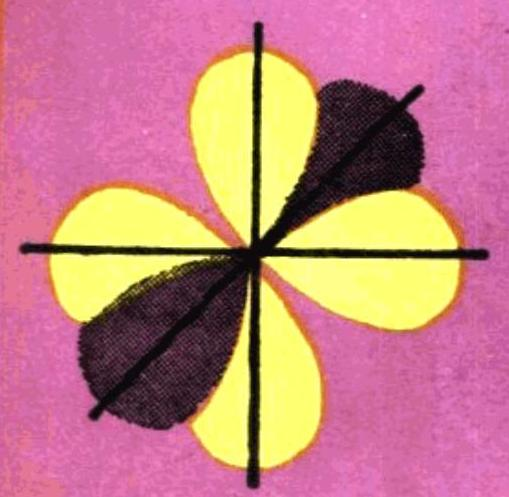
\includegraphics[max width=0.6\textwidth]{images/01912d0f-097c-7e75-8f32-4f326cd86c9f_1_847836.jpg}
\end{center}

第一册静脉细胞减弱 \({R}_{0} = {R}_{0} + {R}_{0}\) \(N = 1/2\) \({K}_{2} = {1.7} \pm {0.2}\) 营销部 销售 \({0.01} \pm {0.02}\) \({0.05} \pm {0.2}\) \(\left| {\psi \left( t\right) }\right| = 1\) 售后的消费价

高级中学课本

(试 用)

化 学

(甲 种 本)

第一册

人民教育出版社化学室编

*

人人名 * * 的 * 出版

北京出版社重印

北京市新华书店发行

中国青年出版社印刷厂印刷 *

\({787} \times {1092}\) 毫米 \({32}\) 开本 \(z\) 分张 \({5.25}\) 插页 2 字数 \({109},{000}\)

1983年11月第 1 版 1987 年 6 月第 4 次印刷

书号: \(\mathrm{K}{7012} \cdot {0528}\) 定价: 0.52 元

\section*{说 明}

本书供六年制中学高中一年级选用, 每周授课 3 课时。

本书是在中小学通用教材化学编写组编的《全日制十年制学校初中课本(试用本)化学》卤素和碱金属一章和《全口制十年制学校高中课本 (试用本) 化学》第一册硫 硫酸、摩尔反应热和物质结构 元素周期律部分内容的基础上, 吸收了几年来各地在试用中的一些教学经验和意见编写成的。

参加本书编写工作的有许国培、程名荣、张健如、胡美玲、 王存志等。北京师范大学化学系的何少华也参加了编写工作。 责任编辑是许国培, 审定者是武永兴、梁英豪。

希望广大教师和研究中学化学教学的同志提出批评和修改意见。

\begin{center}
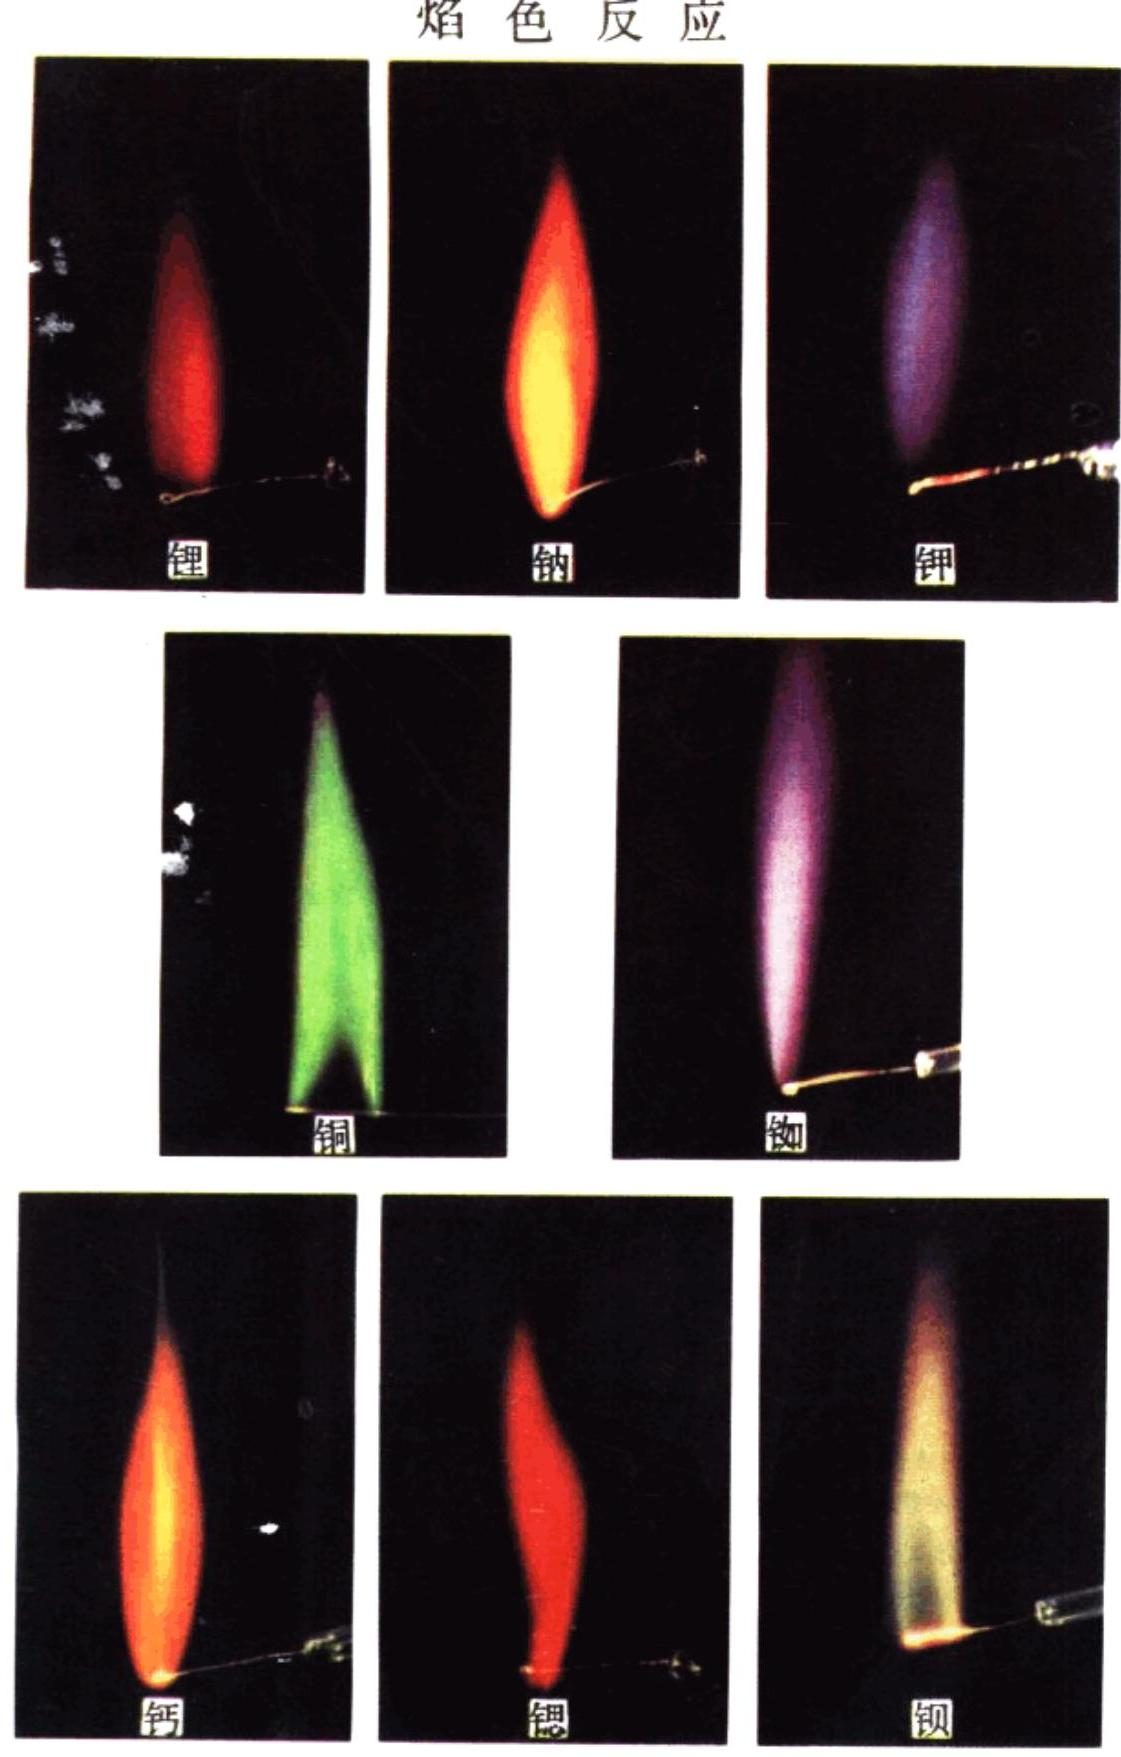
\includegraphics[max width=1.0\textwidth]{images/01912d0f-097c-7e75-8f32-4f326cd86c9f_4_571367.jpg}
\end{center}

\begin{center}
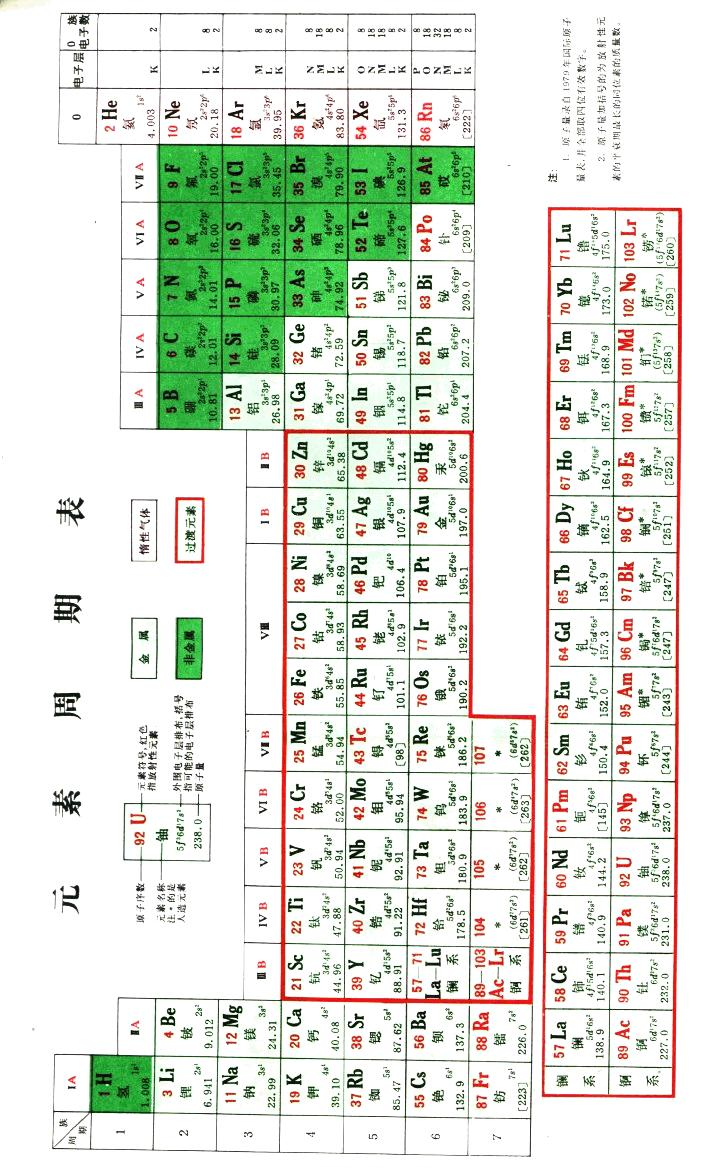
\includegraphics[max width=1.0\textwidth]{images/01912d0f-097c-7e75-8f32-4f326cd86c9f_2_111233.jpg}
\end{center}

\section*{目 录}

1

第一章 摩尔 - 1

第一节 摩尔 -+1

第二节 气体摩尔体积. ..6

第三节 摩尔浓度. .12

第四节 反应热. -18

内容提要. .22

第二章 卤素 .25

第一节 氯气 .25

第二节 氯化氢和盐酸. .31

第三节 氧化-还原反应. .35

第四节 卤族元素. .39

内容提要. - 48

第三章 硫 硫酸 .51

第一节 硫. -51

第二节 硫的氢化物和氧化縣西星街 .54

第三节,硫酸的工业制法——\#\#\#\# .58

第四节 硫酸 硫酸盐. .64

第五节 离子反应 离子方程主要证 .69

第六节 氧族元素. .73

内容提要. .77

第四章 碱金属· - 81

第一节 钠. -81

第二节 钠的化合物. .84

第三节 碱金属元素 -87

内容提要. -.94

第五章 原子结构 元素周期律 .96

第一节 原子核. .96

第二节 核外电子的运动状态. . .99

第三节 原子核外电子的排布. 107

第四节 元素周期律 -115

第五节 元素周期表. .120

第六节 元素周期律的发现和意义 .131

内容提要 -135

学生实验 .145

实验一 化学实验基本操作. .145

实验二 配制一定摩尔浓度的溶液 .148

实验三 重结晶法提纯硫酸铜 测定硫酸铜晶体里结晶

水的含量. .150

实验四 氯、溴、碘的性质. -152

实验五 硫酸的性质 硫酸根离子的检验 -154

实验六 实验习题. -156

实验七 碱金属及其化合物的性质 -157

实验八 同周期、同主族无素性质的递变 -160

实验九 实验习题. -162

选做实验 阿佛加德罗常数的测定 -163

附录 酸、碱和盐的溶解性表 \(\left( {{20}^{ \circ }\mathrm{C}}\right)\) 元素周期表

1 。 ,

\section*{第一章 序}

摩尔是国际单位制的一种基本单位, 它表示物质的量。摩尔广泛地应用于科学研究、工农业生产等等方面。在中学化学里, 摩尔应用于计算微粒的数量、物质的质量、气体的体积、 溶液的浓度、反应过程的热量变化等等。

我们要重视摩尔的学习, 理解摩尔的意义, 学会使用摩尔这个基本单位的方法, 并在以后各章的学习里不断应用。

\section*{第一节 摩 尔}

\section*{一、摩尔}

我们在初中化学里, 学习过原子、分子、离子等构成物质的微粒, 知道单个这样的微粒是肉眼看不见的, 也是难于称量的。但是, 在实验室里取用的物质, 不论是单质还是化合物, 应是看得见的、可以称量的。生产上, 物质的用量当然更大, 常以吨计。物质之间的反应, 既是按照一定个数、肉眼看不见的原子、分子或离子来进行, 而实践上又是以可称量的物质进行反应。所以, 很需要把微粒跟可称量的物质联系起来。

·怎样联系起来呢? 就是要建立一种物质的量的基本单位, 这个单位是含有同数的原子、分子、离子等等的集体。科学上, 已经建立把微粒跟微粒集体联系起来的单位。那么, 采取多大的集体作为物质的量的单位呢?

近年来, 科学上应用 12 克碳-12(或 0.012 千克碳-12)来衡量碳原子集体。碳 -12 就是原子核里有 6 个质子和 6 个中子的碳原子。根据实验测定, 12 克碳-12 含有的原子数就是阿佛加德罗 \({}^{\left( 1\right) }\) 常数。阿佛加德罗常数经过实验已测得比较精确的数值。在这里,采用 \({6.02} \times {10}^{23}\) 这个非常近似的数值。

康尔是表示物质的量的单位, 每摩尔物质含有阿佛加德罗常数个微粒。例如:

1 摩尔 2 的碳原子含有 \({6.02} \times {10}^{23}\) 个碳原子,

1 摩尔的氢原子含有 \({6.02} \times {10}^{23}\) 个氢原子,

1 摩尔的氧分子含有 \({6.02} \times {10}^{23}\) 个氧分子,

1 摩尔的水分子含有 \({6.02} \times {10}^{28}\) 个水分子,

1 摩尔的二氧化碳分子含有 \({6.02} \times {10}^{23}\) 个二氧化碳分子,

1 摩尔的氢离子含有 \({6.02} \times {10}^{23}\) 个氢离子, \(R\)

\(1\) 摩尔的氢氧根离子含有 \({6.02} \times {10}^{29}\) 个氢氧根离子。

阿佛加德罗常数是很大的数值, 但摩尔作为物质的量的单位应用极为方便。因为实验测得 1 摩尔碳-12 的质量是 12 克,即含有 \({6.02} \times {10}^{23}\) 个碳原子的质量。由此我们可以推算 \(1\) 摩尔任何原子的质量。

一种元素的原子量是以碳 -12 的质量的 \(1/{12}\) 作为标准, 其它元素原子的质量跟它相比较所得的数值, 如氧的原子量是 16 , 氢的原子量是 1 , 铁的原子量是 55.85 , 等等。 1 个碳原子的质量跟 1 个氧原子的质量之比是 12:16。1 摩尔 碳原子

① 阿佛加德罗(Avogadrc 1776-1856) 是意大利物理学家。

② 摩尔可以简称为摩, 符号 mol。 跟 1 摩尔氧原子所含有的原子数相同,都是 \({6.02} \times {10}^{28}\) 。1 摩尔碳原子是 12 克, 那么 1 摩尔氧原子就是 16 克。同理, 1 摩尔任何原子的质量就是以克为单位, 数值上等于该种原子的原子量。由此我们可以直接推知:

氢的原子量是 1,1 摩尔氢原子的质量是 1 克,

铁的原子量是 \({55.85},1\) 摩尔铁原子的质量是 55.85 克。

其次, 我们用摩尔来衡量双原子分子或多原子分子构成的各种物质的时候, 那么同样地可以推知, 1 摩尔任何分子的质量, 就是以克为单位, 数值上等于该种分子的分子量。

氢气的分子量是 2,1 摩尔氢气的质量是 2 克,

氧气的分子量是 32,1 摩尔氧气的质量是 32 克,

二氧化碳的分子量是 44,1 摩尔二氧化碳的质量是 44 克,

水的分子量是 18,1 摩尔水的质量是 18 克。

当摩尔应用于表示离子的时候, 同样可以推知 1 摩尔离子的质量。由于电子的质量过于微小, 失去或得到的电子的质量可以略去不计。

1 摩尔 \({\mathrm{H}}^{ + }\) 的质量是 1 克,

1 摩尔 \({\mathrm{{OH}}}^{ - }\) 的质量是 17 克,

1 摩尔 \({\mathrm{{Cl}}}^{ - }\) 的质量是 35.5 克。

对于离子化合物也可以同样推知,如 1 摩尔 \(\mathrm{{NaCl}}\) 的质量是 58.5 克。

总之, 摩尔象一座桥梁把单个的、肉眼看不见的微粒跟很大数量的微粒集体、可称量的物质之间联系起来了。

应用摩尔来衡量物质的量, 在科学技术上带来了方便。如

从化学反应中反应物和生成物之间的原子、分子等微粒的比值, 可以直接知道它们之间摩尔的数目之比,

\[
\underset{1\text{ 摩尔 }1\text{ 摩尔 }}{\mathrm{C} + {\mathrm{O}}_{2}} = {\mathrm{{CO}}}_{2}
\]

\[
\mathrm{{Mg}} + 2\mathrm{{HCl}} = {\mathrm{{MgCl}}}_{2} + {\mathrm{H}}_{2} \uparrow
\]

\[
\text{1 豪尔 2 庫尔 1 摩尔 1 摩尔}
\]

\section*{二、关于家尔质量的计算}

1 摩尔物质的质量通常也叫做该物质的摩尔质量, 摩尔质量的单位是“克/摩尔”。物质的量、物质的质量和摩尔质量之间的关系可以用下式表示:

\[
\text{物质的质量 (克) 库尔) } = \text{ 物质的量 (摩尔) }
\]

[例题 1] 90 克水相当于多少摩尔水分子?

[解] 水的分子量是 18, 水的摩尔质量是 18 克/摩尔。

\[
\frac{90}{{18}\text{ 克 }/\text{ 摩尔 }} = 5\text{ 摩尔 }
\]

答: 90 克水相当于 5 摩尔水, 也可以说 90 克水 所含的摩尔数是 5 。

[例题 2] 2.5 摩尔铜原子的质量是多少克?

[解] 铜的原子量是 63.5, 铜的摩尔质量是 63.5 克/摩尔。

2.5 摩尔铜的质量 \(= {63.5}\) 克 \(/\) 摩尔 \(\times {2.5}\) 摩尔 \(= {158.8}\) 克

答: 2.5 摩尔铜原子 (或简称 2.5 摩尔铜) 的质量等于 158.8 克。

[例题 3] 4.9 克硫酸里含有多少硫酸分子?

[解] 硫酸的分子量是 98 , 硫酸的摩尔质量是 98 克/摩尔。

\[
\frac{{4.9}\text{ 克 }}{{98}\text{ 克 }/\text{ 摩尔 }} = {0.05}\text{ 摩尔 }
\]

4.9 克硫酸的分子数 \(= {6.02} \times {10}^{23}/\) 摩尔 \(\times {0.05}\) 摩尔

\[
= {3.01} \times {10}^{22}
\]

答: 4.9 克硫酸里含有 \({3.01} \times {10}^{22}\) 个分子。

\section*{习 题}

1. 2 个氧分子、2 克氧气、2摩尔氧分子有什么区别?

2. 选择正确的答案填写在括号里。

0.5 摩尔氢气含有( )。

① 0.5 个氢分子,② 1 个氢原子,③ \({6.02} \times {10}^{23}\) 个氢原子,④ \({3.01} \times {10}^{23}\) 个氢分子,⑤ \({3.01} \times {10}^{12}\) 个氢分子。

3. 计算 1 摩尔下列物质的质量。

(1) 氦、镁、氯原子、磷原子。

(2). 硝酸、硝酸铵、蔗糖 \(\left( {{\mathrm{C}}_{12}{\mathrm{H}}_{22}{\mathrm{O}}_{11}}\right)\) 。

4. 下列物质的量各等于多少摩尔。

(1) 1 千克硫原子, 0.5 千克铝原子, 0.25 千克锌原子。

(2) 22 克二氧化碳, 500 克氯化钠, 1.5 千克蔗糖。

5. 分别列出铝、铁、铅的摩尔质量。根据 \({20}^{ \circ }\mathrm{C}\) 时,铝、 铁、铅 的 密度 ① 分别是 2.70 克/厘米 \({}^{3}\text{、}{7.86}\) 克/厘米 \({}^{3}\text{、}{11.3}\) 克/厘米 \({}^{3}\) ,计算 1 摩尔铝、铁、铅的体积。

\customfootnote{

① 按照国际单位制,密度的单位应是千克每立方米 \(\left( {\mathrm{{kg}}/{\mathrm{m}}^{3}}\right)\) ,在这里,暂按习惯用克每立方厘米 \(\left( {\mathrm{g}/{\mathrm{{cm}}}^{3}}\right)\) 或克每升 \(\left( {\mathrm{g}/\mathrm{l}}\right)\) 为单位。

}

6. 在 \({15}^{ \circ }\mathrm{C}\) 时,蔗糖的密度是 1.588 克/厘米 \({}^{8}\) ,计算 1 摩尔蔗糖的体积。

7. 分解氯酸钾制氧气的时候, 制 0.6 摩尔氧气需要多少摩尔的氯酸钾?

8. 跟含 4 克氢氧化钠的溶液起反应使生成正盐, 需用下列酸各多少摩尔。

(1) \(\mathrm{{HCl}}\) (2) \({\mathrm{{HNO}}}_{3}\) (3) \({\mathrm{H}}_{2}{\mathrm{{SO}}}_{4}\)

(4) \({\mathrm{H}}_{3}{\mathrm{{PO}}}_{4}\) (5) \({\mathrm{{HClO}}}_{3}\) (氢酸)

9. 硫酸铵、硝酸铵、磷酸氢二铵 \(\left\lbrack {{\left( {\mathrm{{NH}}}_{4}\right) }_{2}{\mathrm{{HPO}}}_{4}}\right\rbrack\) 、尿素都可以作为氮肥。试计算:

(1) 1 摩尔上述物质的质量各是多少充。

(2)1 摩尔上述物质里各含多少摩尔氮原子。

\section*{第二节 气体摩尔体积}

\section*{一、气体摩尔体积}

对于固态或液态的物质来说, 1 摩尔各种物质的体积是不相同的。例如, \({20}^{ \circ }\mathrm{C}\) 时,1 摩尔铁的体积是 7.1 厘米 \({}^{3},1\) 摩尔铝的体积是 10 厘米 \({}^{8},1\) 摩尔铅的体积是 18.3 厘米 \({}^{8}\) (图 1-1); 1 摩尔水的体积是 18.0 厘米 \({}^{8},1\) 摩尔纯硫酸的体积是 54.1 厘米 ,1 摩尔蔗糖的体积是 215.5 厘米 * (图 1-2)。

1 摩尔固态或液态的物质的体积为什么不同呢? 这因为对固态或液态的物质来说, 构成它们的微粒间的距离是很小的, 1 摩尔物质的体积主要决定于原子、分子或离子的大小。 构成不同物质的原子、分子或离子的大小是不同的, 所以它们

\begin{center}
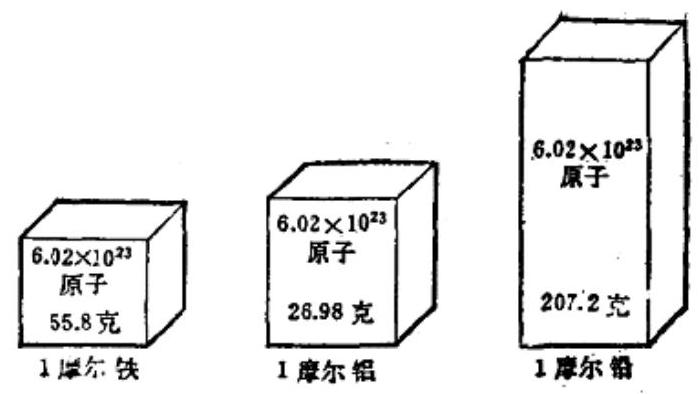
\includegraphics[max width=0.8\textwidth]{images/01912d0f-097c-7e75-8f32-4f326cd86c9f_14_662342.jpg}
\end{center}

图 1-1 1 摩尔的几种金属

\begin{center}
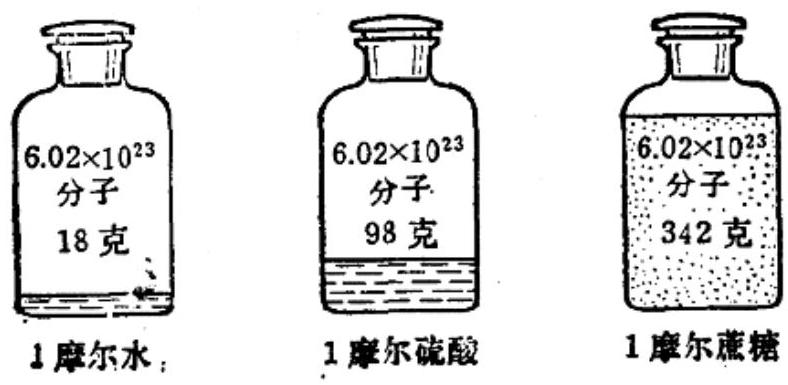
\includegraphics[max width=0.9\textwidth]{images/01912d0f-097c-7e75-8f32-4f326cd86c9f_14_118708.jpg}
\end{center}

图 1-2 1 摩尔的几种化合物

1 摩尔的体积也就有所不同。

但是, 对气体来说, 情况就大不相同。

我们分别计算 1 摩尔氢气、氧气和二氧化碳在标准状况 \(\Phi\) 时的体积。氢气的摩尔质量是 2 克/摩尔. 氧气的摩尔质量是 32 克/摩尔, 二氧化碳的摩尔质量是 44 克/摩尔, 同时它们的密度分别是 0.0899 克/升、1.429 克/升和 1.977 克/升。这样就可以算出上述气体在标准状况时所占的体积。

\customfootnote{

① 标准状况是指压强为 1 标准大气压和温度为 \({0}^{ \circ }\mathrm{C}\) 。根据国际单位制压强单位是帕斯卡(Pa)。在这里暂用标准大气压 (atm)。1 atm \(= {101325}\mathrm{\;{Pa}}\) 。

}

氢气的摩尔体积 \(= \frac{{2.016}\text{ 克 }/\text{ 摩尔 }}{{0.0899}\text{ 克 }/\text{ 升 }} = {22.4}\) 升 \(/\) 摩尔

氧气的摩尔体积 \(= \frac{{32.0}\text{ 克 }/\text{ 摩尔 }}{{1.429}\text{ 克 }/\text{ 升 }} = {22.4}\) 升 \(/\) 摩尔

二氧化碳的摩尔体积 \(= \frac{{44.0}\text{ 克 }/\text{ 摩尔 }}{{1.977}\text{ 克 }/\text{ 升 }} = {22.3}\) 升 \(/\) 摩尔

从上面几个例子可以看出, 在标准状况时, 1 摩尔三种气体的体积都约是 22.4 升。而且经过许多实验发现和证实, 1 摩尔的任何气体在标准状况下所占的体积都约是 22.4 升 (图 1-3)。

\begin{center}
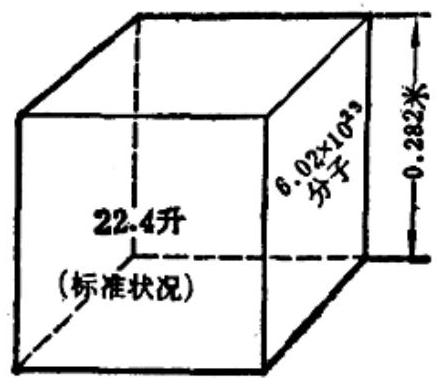
\includegraphics[max width=0.5\textwidth]{images/01912d0f-097c-7e75-8f32-4f326cd86c9f_15_661945.jpg}
\end{center}

图 1-3 气体摩尔体积

\begin{center}
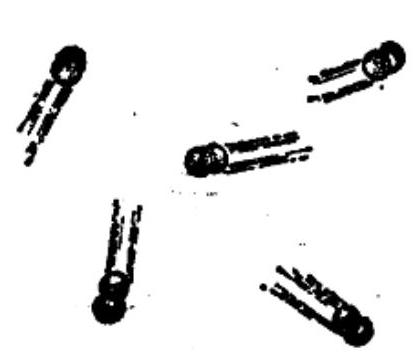
\includegraphics[max width=0.5\textwidth]{images/01912d0f-097c-7e75-8f32-4f326cd86c9f_15_326194.jpg}
\end{center}

图 1-4 气体分子的运动和距离

在标准状况下, 1摩尔的任何气体所占的体积都约是 22.4 升, 这个体积叫做气体摩尔体积。

为什么 1 摩尔的固体、液体的体积各不相同, 而 1 摩尔气体在标准状况时所占的体积都相同呢? 这要从气态物质的结构去找原因。气体的分子在较大的空间里迅速地运动着(图 1-4)。在通常情况下气态物质的体积要比它在液态或固态时大 1000 倍左右, 这是因为气体分子间有着较大的距离。通常情况下一般气体的分子直径约是 \(4 \times {10}^{-{10}}\) 米,分子间的平均距离约是 \(4 \times {10}^{-9}\) 米,即平均距离是分子直径的 10 倍 左 右 (图 1-5)。这就可以推知, 气体体积主要决定于分子间的平均距离, 而不象液体或固体那样, 体积主要决定于分子的大小。在标准状况下, 不同气体分子间的平均距离几乎是相等的, 所以任何物质的气体摩尔体积都约是 22.4 升/摩尔。

\begin{center}
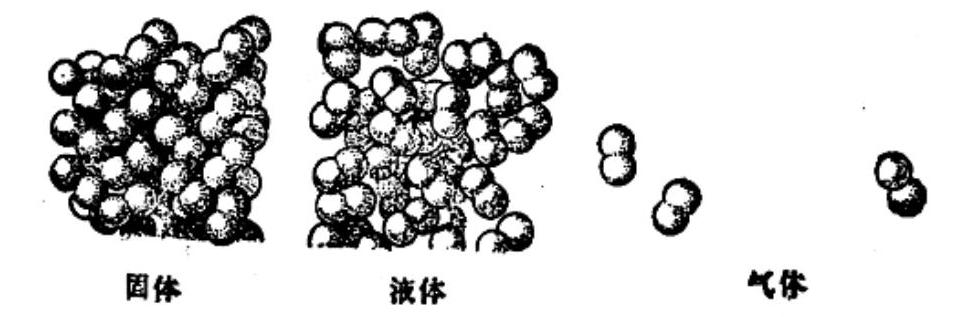
\includegraphics[max width=1.0\textwidth]{images/01912d0f-097c-7e75-8f32-4f326cd86c9f_16_685048.jpg}
\end{center}

图 1-5 固体、液体跟气体的分子间距离比较示意图 (以碘为例)

气体摩尔体积约是 22.4升/摩尔, 为什么一定要加上标准状况这个条件呢: 这是因为气体的体积较大地受到温度和压强的影响。 温度升高时, 气体分子间的平均距离增大, 温度降低时平均距离减小; 压强增大时, 气体分子间的平均距离减小, 压强减小时, 平均距离增大。各种气体在一定温度和压强下, 分子间的平均距离是相等的。在一定的温度和压强下. 气体体积的大小只随分子数的多少而变化, 相同的体积含有相同的分子数。这是经过生产上和科学实验的许多事实所证明的。

在相同的温度和压强下,相同体积的任何气体都含有相同数目的分子, 这就是阿佛加德罗定律。

[讨论] 如果已经知道水的分子式是 \({\mathrm{H}}_{2}\mathrm{O}\) ,我们能够根

据氢气跟氧气化合成水蒸气的体积比是 \(2 : 1 : 2\) ,应用阿佛加德罗定律来证明 1 个氧分子里含有 2 个氧原子吗?

\section*{二、关于气体摩尔体积的计算}

[例题 1] 5.5 克氨相当于多少摩尔氨, 在标准状况时它的体积应是多少升?

【解】氨的分子量是 17, 氨的摩尔质量是 17 克/摩尔。

\[
\frac{5.5}{{17}\text{ 克/摩尔 }} = {0.32}\text{ 摩尔 }
\]

5.5 克氨的体积 \(= {22.4}\) 升/摩尔 \(\times {0.32}\) 摩尔 \(= {7.2}\) 升

答: 5.5 克氨相当于 0.32 摩尔的氨, 在标准状况时, 它的体积是 7.2 升。

[例题 2] 在实验室里使稀盐酸跟锌起反应, 在标准状况时生成 3.36 升氢气。计算需要多少摩尔的 \(\mathrm{{HCl}}\) 和锌。

[解] 设 \(x\) 为所需多少摩尔的锌, \(y\) 为所需多少摩尔的 \(\mathrm{{HCl}}\) 。

\[
\mathrm{{Zn}} + 2\mathrm{{HCl}} = {\mathrm{{ZnCl}}}_{2} + {\mathrm{H}}_{2} \uparrow
\]

1 摩尔 2 摩尔 22.4 升

3.36 升

\[
z = \frac{1\text{ 摩尔 } \times {3.36}\text{ 升 }}{{22.4}\text{ 升 }} = {0.15}\text{ 摩尔 }
\]

\[
y = \frac{2\text{ 摩尔 } \times {3.36}\text{ 升 }}{{22.4}\text{ 升 }} = {0.30}\text{ 摩尔 }
\]

答: 需 0.15 摩尔锌和 0.30 摩尔 \(\mathrm{{HCl}}\) 。

[例题 3] 在标准状况时, 0.20 升的容器里所含一氧化碳的质量为 0.25 克, 计算一氧化碳的分子量。

根据摩尔体积可以计算出一氧化碳的摩尔质量, 而摩尔质量的数值就等于它的分子量。

[解] 一氧化碳的摩尔质量 \(=\) 一氧化碳的密度 \(\times\) 一氧化碳的摩尔体积 \(= \frac{0.25}{0.20}\) 克 \(\times {22.4}\) 升/摩尔 \(= {28}\) 克/摩尔

一氧化碳的分子量 \(= {28}\)

答: 一氧化碳的分子量是 28 。

\section*{习 题}

1. 改正下列说法里可能有的错误, 并说明理由。

(1) .1 摩尔任何气体的体积都是 22.4 升。

(2) 1 摩尔氢气的质量是 1 克, 它所占的体积是 22.4 升。

(3) 1 摩尔任何物质在标准状况时所占的体积都约是 22.4 升。

(4) 1 摩尔氢气和 1 摩尔水所含的分子数相同, 在标准被沉时所占体积都约是 22.4 升。

2. 在标准状况时, 1 升氮气的含有多少个氮分子?

3. 在标准状况时, 15 克氟气所占的体积比 1 克氢气所占的体积是大还是小?

4. 在标准状况时, 4.4 克二氧化碳的体积跟多少克氧气的体积相等?

5. 在实验室制备氢气的时候, 用 0.1 摩尔的锌跟足量稀盐酸起反应, 计算所产生的氢气的体积(在标准状况)。

6. 氮气在标准状况时的密度是 1.25 克/升, 液态氮在 \(- {195.8}^{ \circ }\mathrm{C}\) 的密度是 0.808 克/厘米 \({}^{3}\) ,面态氮在 \(- {232.5}^{ \circ }\mathrm{C}\) 的密度是 1.026 克/厘米 \({}^{3}\) ,比较 1 摩尔的氮在气态、液态、圈态各占多少体积。

7. 在标准状况时, 235 毫升某种气体的质量是 0.406 克, 计算这种气体的分子量。

\section*{第三节 摩 尔 浓 度}

\section*{一、摩尔浓度}

我们在初中化学里学习过百分比浓度, 应用这种表示溶液浓度的方法, 可以了解和计算一定质量的溶液中所含溶质的质量。但是, 我们在许多场合取用溶液时, 一般不是去称它的质量而是量它的体积。同时, 物质起反应时, 反应物和生成物各是多少摩尔相互之间有一定的关系; 知道一定体积溶液里含多少摩尔溶质, 运算起来很便利。因此, 摩尔浓度是生产上和科学实验上常用的一种表示溶液浓度的重要方法。

以 1 升溶液里含有多少摩尔溶质来表示的溶液浓度叫摩尔浓度。摩尔浓度 \({}^{\left( \mathrm{D}\right) }\) 通常用 \(M\) 表示。

\[
\text{摩尔浓度}\left( M\right) = \frac{\text{ 溶质的量 (摩尔) }}{\text{ 溶液的体积 (升) }}
\]

1 升溶液中含 1 摩尔的溶质, 这种溶液就是 1 摩尔浓度的溶液,通常用 \({1M}\) 表示。如蔗糖的摩尔质量是 342 克/摩尔。 把 342 克蔗糖溶解在适量水里配成 1 升溶液, 它的摩尔浓度就是 1 摩尔/升或 \(1{M}_{0}1\) 升溶液中含 171 克蔗糖,它的摩尔浓度就是 \({0.5}\mathrm{M}\) 。又如 1 摩尔的氯化钠的质量是 58.5 克,把 58.5 克氯化钠溶解在适量水里制成 1 升溶液时, 它的摩尔浓度就是 \({1M}\) 。1 升溶液中含 29.3 克氯化钠的溶液浓 度 就是 \({0.5}\mathrm{M}\) 。

\customfootnote{

① 按照国际单位制的规定, 物质的量浓度的单位是摩尔每立方米 \(\left( {\mathrm{{mol}}/{\mathrm{m}}^{3}}\right)\) 。在这里仍暂按习惯沿用摩尔浓度,单位也用摩尔每升 \(\left( {\mathrm{{mol}}/\mathrm{l}}\right)\) 。

}

溶液用摩尔浓度表示时, 常简称为摩尔溶液。

[实验 1-1] 在天平上称出 29.3 克氯化钠, 把称好的氯化钠放在烧杯里, 用适量蒸馏水使它完全溶解。把制得的溶液小心地注入 1000 毫升的容量瓶(图 1-6)。用蒸馏水洗涤烧杯内壁两次, 把每次洗下来的水都注入容量瓶。振荡容量瓶里的溶液使混和均匀。然后缓缓地把蒸馏水直接注入容量瓶直到液面接近刻度 2-3 厘米处。改用胶头滴管加水到瓶颈刻度的地方, 使溶液的凹面正好跟刻度相平。把容量瓶塞好, 反复摇匀。

\begin{center}
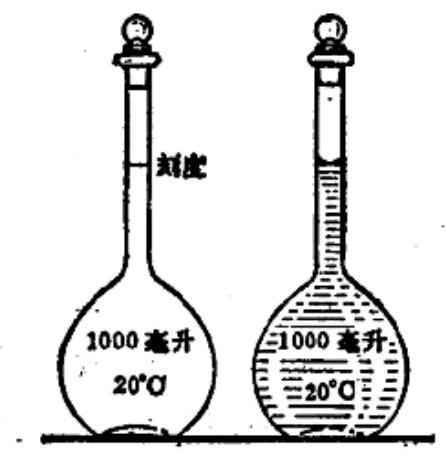
\includegraphics[max width=0.5\textwidth]{images/01912d0f-097c-7e75-8f32-4f326cd86c9f_20_483453.jpg}
\end{center}

图 1-6 配制摩尔浓度的溶液

这样配制成的溶液就是 \({0.5}\frac{M}{r}\) 的氯化钠溶液。 \(\xi\) .

\section*{二、在摩尔溶液中溶质微粒的数目}

1 摩尔任何物质的微粒数都是 \({6.02} \times {10}^{23}\) 。 1 升 1 M 的蔗糖溶液含有 \({6.02} \times {10}^{23}\) 个蔗糖分子。对于非电解质来说,体积相同的同摩尔浓度的溶液都应含有相同的溶质分子数。

但是, 对于溶质为离子化合物或在水里完全电离的共价化合物等电解质来说, 情况就比较复杂。例如, 氯化钠溶解在水里电离为 \({\mathrm{{Na}}}^{ + }\) 和 \({\mathrm{{Cl}}}^{ - }\) 。所以,1 升 \({1M}\) 的 \(\mathrm{{NaCl}}\) 溶液含有 \({6.02} \times {10}^{23}\) 个 \({\mathrm{{Na}}}^{ + }\) 和 \({6.02} \times {10}^{23}\) 个 \({\mathrm{{Cl}}}^{ - }\) 。同样地,1 升 \({1M}\) 的 \(\mathrm{{NaOH}}\) 溶液含有 \({6.02} \times {10}^{23}\) 个 \({\mathrm{{Na}}}^{ + }\) 和 \({6.02} \times {10}^{23}\) 个 \({\mathrm{{OH}}}^{ - }\) ; 1 升 \({1M}\) 的 \({\mathrm{{CaCl}}}_{2}\) 溶液含有 \({6.02} \times {10}^{23}\) 个 \({\mathrm{{Ca}}}^{2 + }\) 和 \(2 \times {6.02} \times\) \({10}^{23}\) 个 \({\mathrm{{Cl}}}^{ - }\) 。又例如 1 升 \({1M}\) 的 \(\mathrm{{HCl}}\) 溶液里含有 \({6.02} \times {10}^{23}\) 个 \({\mathrm{H}}^{ + }\) 和 \({6.02} \times {10}^{23}\) 个 \({\mathrm{{Cl}}}^{ - }\) 。

\section*{三、关于摩尔浓度的计算}

1. 已知溶质的质量和溶液的体积, 计算溶液的摩尔浓度。

[例题 1] 在 200 毫升稀盐酸里溶有 0.73 克 \(\mathrm{{HCl}}\) ,计算溶液的摩尔浓度。

摩尔浓度所表示的就是 1 升溶液里含多少摩尔溶质, 在这题里, 就是要算出 1 升溶液里含多少摩尔的 HCl。

[解] \(\mathrm{{HCl}}\) 的分子量是 36.5,它的摩尔质量是 36.5 克/摩尔。0.73 克 \(\mathrm{{HCl}}\) 相当于:

\[
\frac{{0.73}\text{ 克 }}{{36.5}\text{ 克/摩尔 }} = {0.02}\text{ 摩尔 }
\]

1000 毫升溶液中含 \(\mathrm{{HCl}}\)

\[
\text{0.02 摩尔} \times \frac{1000}{200}\text{毫升} = {0.1}\text{摩尔}
\]

答: 这种稀盐酸的浓度是 \({0.1}{M}_{ \circ }\)

2. 已知溶液的摩尔浓度, 计算一定体积的溶液里所含溶

质的质量。

[例题 2] 计算配制 500 毫升 \({0.1}\mathrm{M}\) 的 \(\mathrm{{NaOH}}\) 溶液所需 \(\mathrm{{NaOH}}\) 的质量。

[解] \(\mathrm{{NaOH}}\) 的分子量是 40,它的摩尔质量是 40 克/摩尔。

0.1 摩尔的 \(\mathrm{{NaOH}}\) 的质量 \(= {40}\) 克/摩尔 \(\times {0.1}\) 摩尔 \(= 4\) 克

500 毫升 \({0.1}\mathrm{M}\mathrm{{NaOH}}\) 溶液所含 \(\mathrm{{NaOH}}\) 的质量是:

\[
\frac{{500}\text{ 毫升 } \times 4\text{ 克 }}{{1000}\text{ 毫升 }} = 2\text{ 克 }
\]

答: 制备 500 毫升 \({0.1}\mathrm{M}\) 的 \(\mathrm{{NaOH}}\) 溶液需 2 克 \(\mathrm{{NaOH}}\) 。

3. 应用摩尔浓度作关于浓溶液稀释的计算。

[例题 3] \({20}\%\) 的蔗糖溶液 200 克,加适量的水稀释到 1 升, 计算稀释后蔗糖溶液的摩尔浓度。

[解] 蔗糖 \(\left( {{\mathrm{C}}_{12}{\mathrm{H}}_{22}{\mathrm{O}}_{11}}\right)\) 的分子量是 342,蔗糖的摩尔质量是 342 克/摩尔。

溶液里所含蔗糖的质量是 200 克 \(\times {20}\% = {40}\) 克

\[
\frac{40}{{342}\text{ 克 }/\text{ 摩尔 }} = {0.117}\text{ 摩尔 }
\]

1 升蔗糖溶液里含有 0.117 摩尔蔗糖。

答: 蔗糖溶液的摩尔浓度是 \({0.117M}\) 。

[例题 4] 计算配制 500 毫升 \(1\mathrm{M}\) 的硫酸溶液需要密度为 1.836 克/厘米 \({}^{3}\) 的浓硫酸 \(\left( {{98}\% {\mathrm{H}}_{2}{\mathrm{{SO}}}_{4}}\right)\) 多少毫升?

浓硫酸稀释后,所含 \({\mathrm{H}}_{2}{\mathrm{{SO}}}_{4}\) 的质量是不变的,因而在硫酸溶液里多少摩尔 \({\mathrm{H}}_{2}{\mathrm{{SO}}}_{4}\) 等于浓硫酸里多少摩尔的 \({\mathrm{H}}_{2}{\mathrm{{SO}}}_{4}\) 。 先算出硫酸溶液里含多少摩尔 \({\mathrm{H}}_{2}{\mathrm{{SO}}}_{4}\) ,再算出浓硫酸的摩尔浓度,从所含多少摩尔 \({\mathrm{H}}_{2}{\mathrm{{SO}}}_{4}\) 可以算出需要的浓硫酸的体积。

[解] 硫酸溶液中含 \({\mathrm{H}}_{2}{\mathrm{{SO}}}_{4}\)

\[
\frac{500}{1000}\text{毫升} \times 1\text{摩尔} = {0.5}\text{摩尔}
\]

硫酸的摩尔质量 \(= {98}\) 克/摩尔

1000 毫升浓硫酸中 \({\mathrm{H}}_{2}{\mathrm{{SO}}}_{4}\) 的质量

\(= {1000}\) 毫升 \(\times {1.836}\) 克/毫升 \(\times \frac{98}{100} = {1799}\) 克

1000 毫升浓硫酸里含 \({\mathrm{H}}_{2}{\mathrm{{SO}}}_{4}\)

\[
\frac{{1799}\text{ 克 }}{{98}\text{ 克/摩尔 }} = {18.4}\text{ 摩尔 }
\]

含 0.5 摩尔 \({\mathrm{H}}_{2}{\mathrm{{SO}}}_{4}\) 的浓硫酸的体积

\[
= \frac{{0.5}\text{ 摩尔 }}{{18.4}\text{ 摩尔 }/\text{ 升 }} = {0.0272}\text{ 升 } = {27.2}\text{ 毫升 }
\]

答: 需要浓硫酸 \(\left( {{98}\% {\mathrm{H}}_{2}{\mathrm{{SO}}}_{4}}\right) {27.2}\) 毫升。

4. 已知起反应的两种溶液的摩尔浓度以及其中一种溶液的体积, 计算另一种溶液的体积。

[例题 5] 中和 1 升 \({0.5M}\mathrm{{NaOH}}\) 溶液,需要多少升的 \({1M}{\mathrm{H}}_{2}{\mathrm{{SO}}}_{4}\) 溶液?

[解] \(2\mathrm{{NaOH}} + {\mathrm{H}}_{2}{\mathrm{{SO}}}_{4} = {\mathrm{{Na}}}_{2}{\mathrm{{SO}}}_{4} + 2{\mathrm{H}}_{2}\mathrm{O}\)

2 家尔 \(\;1\) 摩尔

1 升 \({0.5M}\) 溶液中含 \(\mathrm{{NaOH}}\)

1 升 \(\times {0.5}\) 摩尔 \(/\) 升 \(= {0.5}\) 摩尔

中和 0.5 摩尔 \(\mathrm{{NaOH}}\) 需 \({\mathrm{H}}_{2}{\mathrm{{SO}}}_{4}\)

\(0,5\) . 摩尔 \(\times 1/2 = {0.25}\) 摩尔.

含 0.25 摩尔的 \(1{\mathrm{{MH}}}_{2}{\mathrm{{SO}}}_{4}\) 溶液的体积

\[
= \frac{1\text{ 升 } \times {0.25}\text{ 摩尔 }}{1\text{ 摩尔 }} = {0.25}\text{ 升 }
\]

答: 中和 \(1\mathrm{升},{0.5M}\mathrm{{NaOH}}\) 溶液需 \({1M}{\mathrm{H}}_{2}{\mathrm{{SO}}}_{4}\) 溶液 0.25 升。

\section*{习 题}

1. 制备下列各物质的 \({0.2}\mathbf{M}\) 溶液各 50 毫升,需用下列物质各多少克?

(1) \({\mathrm{{HClO}}}_{3}\left( 2\right) {\mathrm{H}}_{2}{\mathrm{{SO}}}_{4}\left( 3\right) {\mathrm{{Na}}}_{2}{\mathrm{{SO}}}_{4}\left( 4\right) {\mathrm{{FeSO}}}_{4} \cdot 7{\mathrm{H}}_{2}\mathrm{O}\)

2. 在下列各种溶液里取用溶质1克, 各需溶液多少毫升?

(1) \({0.1M}{\mathrm{H}}_{2}{\mathrm{{SO}}}_{4}\) 溶液 -(2) \({3M}\mathrm{{KOH}}\) 溶液

(B) \({0.2M}{\mathrm{{BaCl}}}_{2}\) 溶液 (4) \({0.5M}{\mathrm{{Na}}}_{2}{\mathrm{{SO}}}_{4}\) 溶液

3. 下列说法是否正确, 说明理由。

(1)体积相同、摩尔浓度相同的任何物质的溶液含有相同的分子数。

(2) 10 毫升 \({1M}\) 硫酸溶液比 100 毫升 \({1M}\) 硫酸溶液的浓度小。

(3) 100 毫升 0.1 M 硫酸溶液和 50 毫升 1 M 硫酸溶液分别跟 50 毫升 \({1M}{\mathrm{{BaCl}}}_{2}\) 溶液起反应,前者生成的 \({\mathrm{{BaSO}}}_{4}\) 沉淀多。

4. 中和 4 克氢氧化钠, 用去盐酸 25 毫升, 计算这种盐酸的摩尔浓度。

5. 某种待测浓度的NaOH溶液25毫升,加入20毫升1M 的 \({\mathrm{H}}_{2}{\mathrm{{SO}}}_{4}\) 溶液后已显酸性,再滴入 \({1M}\;\mathrm{{KOH}}\) 溶液 1.5 毫升才达到中和。计算待测浓度的 NaOH 溶液的摩尔浓度。

6. \({37}\%\) 的盐酸 (密度 1.19 克/厘米 \({}^{3}\) ) 相当于多少摩尔浓度的盐酸?

7. 实验室常用的 \({65}\%\) 浓硝酸,密度为 1.4 克/厘米 \({}^{5}\) ,计算它的摩尔浓度。要配制 \({3M}\) 的硝酸 100 毫升,需用这种浓硝酸多少毫升?

\section*{第四节 反 应 热}

\section*{一、热化学方程式}

化学反应都伴随着能量的变化, 通常表现为热量的变化, 即有放热或吸热的现象发生。反应过程中放出或吸收的热都属于反应热。远古时代, 人类的祖先守着一堆篝火, 烘烤食物, 寒夜取暖, 这就是利用燃烧放出的热。到了近代; 利用化学反应的热能的规模 \(\theta\) -益扩大了。 \(\because\) 煤炭、石油、天然气等能源不断开发出来, 作为燃料和动力, 用来开动火车、汽车、飞机。 拖拉机、联合收割机, 开动工厂里的各种机器, 并供日常生活中做饭、取暖之用。现代, 这些能源正在以更大的规模被利用着。总而言之, 化学反应放出的热能对我们是极为重要的。

化学反应里有原子和原子的重新结合, 反应过程里放出或吸收的热量都和原子跟原子的分离和结合联系着。例如, 碳跟氧气的反应里,碳原子跟氧分子里的氧原子结合就会导致热量的产生。人们通常应用摩尔这个物质的量的单位来计算可称量物质在反应过程里放出或吸收的热量。这是把微粒跟可测量的热量联系起来的一个例子。通过实验, 测得 1 摩尔碳 \(\left( {{6.02} \times {10}^{23}\text{个碳原子}}\right)\) 跟 1 摩尔氧气 \(\left( {{6.02} \times {10}^{23}}\right.\) 个氧分子) 起反应,生成 1 摩尔二氧化碳 \(\left( {{6.02} \times {10}^{23}}\right.\) 个 \({\mathrm{{CO}}}_{2}\) 分子), 放出 94 千卡 \(\text{①}\) 的热。 2 摩尔氢气跟 1 摩尔氧气起反应,生成 2 摩尔水蒸气, 放出 115.6 千卡的热。

\[
\mathrm{C}\text{ (固) } + {\mathrm{O}}_{2}\left( \text{ 气 }\right) = {\mathrm{{CO}}}_{2}\left( \text{ 气 }\right) + {94}\text{ 千卡 }
\]

\[
2{\mathrm{H}}_{2}\left( \text{气}\right) + {\mathrm{O}}_{2}\left( \text{气}\right) = 2{\mathrm{H}}_{2}\mathrm{O}\left( \text{气}\right) + {115.6}\text{千卡}
\]

上面的反应是放热的, 也有一些反应是吸热的。当水蒸气跟灼热的碳接触时, 发生的反应就要吸收热量。

\[
\underset{1\text{ 摩尔 }}{\mathrm{C}\left( \text{ 固 }\right) } + \underset{1\text{ 摩尔 }}{{\mathrm{H}}_{2}\mathrm{O}\left( \text{ 气 }\right) } = \underset{1\text{ 摩尔 }}{\mathrm{{CO}}\left( \text{ 气 }\right) } + \underset{1\text{ 摩尔 }}{{\mathrm{H}}_{2}\left( \text{ 气 }\right) } - {31.4}\text{ 千卡 }
\]

1 摩尔的碳跟 1 摩尔的水蒸气起反应, 吸收 31.4 千卡的热量。

在化学方程式里, 为什么要在物质的右边注明固、液、气等状态呢? 我们知道, 物质呈现哪一种聚集状态是跟它们含有的能量有关的。为了精确起见, 要注明反应物和生成物的状态才能确定放出或吸收的热量多少。例如:

\[
2{\mathrm{H}}_{2}\left( {E\left( \right) + {\mathrm{O}}_{2}\left( {AE}\right) }\right) = 2{\mathrm{H}}_{2}\mathrm{O}\left( {AE}\right) + {115.6}\text{千卡}
\]

\[
2{\mathrm{H}}_{2}\left( 气\right) + {\mathrm{O}}_{2}\left( 气\right) = 2{\mathrm{H}}_{2}\mathrm{O}\left( 液\right) + {136.6}\text{千卡}
\]

放出的热量用“ + ”号表示, 吸收的热量用 “一” 号表示。 这种表明反应所放出或吸收的热量的化学方程式叫做热化学方程式。

应用热化学方程式可以计算生产上出现的热量的变化。 例如, 可以计算甲烷燃烧所放出的热量。在生产上, 很注意反

① 按照国际单位制, 热量的单位是焦耳(J)。在这里暂时仍沿用卡 (cal) 作为热量单位。 \(1\mathrm{{cal}} = {4.184}\mathrm{\;J}\) 。所列反应放出或吸收的热量的数据一般是指在 1 标准大气压和 \({25}^{ \circ }\mathrm{C}\) 的条件下测得的热量。以下同。 应所放出的热量的充分利用。

[例题] 1 摩尔甲烷燃烧时, 生成液态水和二氧化碳, 同时放出 212.8 千卡的热。计算燃烧 1000 升 (标准状况) 甲烷所产生的热量。

[解] 1000 升甲烷燃烧所产生的热量

\[
= \frac{{1000}\text{ 升 }}{{22.4}\text{ 升 }} \times {212.8}\text{ 千卡 } = {9.50} \times {10}^{8}\text{ 千卡 }
\]

答: 1000 升 (标准状况) 甲烷燃烧所放出的热是 \({9.50} \times {10}^{8}\) 千卡。

\section*{二、燃烧热}

由于反应的情况不同, 反应热可以分为许多种, 如燃烧热、中和热等。在这里, 只介绍燃烧热。

许多单质或化合物在燃烧时放出热量, 生成稳定的物质, 如二氧化碳, 水、氯化氢等等。

1 摩尔物质完全燃烧时所放出的热量, 叫做该物质的 燃烧热。燃烧热通常可由实验测得。例如, 测得 1 摩尔碳完全燃烧放出的热量是 94 千卡, 这就是碳的燃烧热。

\[
\mathrm{C}\left( \text{固}\right) + {\mathrm{O}}_{2}\left( \text{气}\right) = {\mathrm{{CO}}}_{2}\left( \text{气}\right) + {94}\text{千卡}
\]

由实验测得, 1 摩尔氢气燃烧而生成液态水, 放出的热量是 68.3 千卡, 68.3 千卡就是氢气的燃烧热。

\[
{\mathrm{H}}_{2}\left( \text{ 气 }\right) + \frac{1}{2}{\mathrm{O}}_{2}\left( \text{ 气 }\right) = {\mathrm{H}}_{2}\mathrm{O}\text{ (液) } + {68.3}\text{ 千卡 }
\]

在计算燃烧热时, 可燃物质是以 1 摩尔作为标准来计算的, 所以热化学方程式里的元素符号或分子式前面的系数可以用分数表示。

由实验测得, 1 摩尔气态一氧化碳燃烧而生成气态二氧化碳时, 放出 67.6 千卡的热。

\[
\mathrm{{CO}}\left( \text{ 气 }\right) + \frac{1}{2}{\mathrm{O}}_{2}\left( \text{ 气 }\right) = {\mathrm{{CO}}}_{2}\left( \text{ 气 }\right) + {67.6}\text{ 千卡 }
\]

一氧化碳的燃烧热就是 67.6 千卡。

学习反应热概念, 能够帮助我们理解反应中的热量变化, 也是开始通过能量变化来了解物质性质及其反应过程。

\section*{习 题}

1. 在足量氧气里燃烧 2.5 摩尔的碳, 生成二氧化碳, 能放出多少千卡的热量?

2. 要燃烧多少摩尔的氢气, 生成液态水. 才能得到 1000 千卡的热量?

3. 比较燃烧氢气(生成液态水)和碳(生成二氧化碳)各1 千克所放出的热量?

4. 燃烧 1 克甲烷 \(\left( {\mathrm{{CH}}}_{4}\right.\) ,气体),生成液态水和二氧化碳能放出 13.3 千卡的热量,计算燃烧 5 摩尔甲烷能放出多少热量。

5. 燃烧 1 克乙炔 \(\left( {{\mathrm{C}}_{2}{\mathrm{H}}_{2}\text{,气体}}\right)\) ,生成液态水和二氧化碳能放出 11.9 千卡的热量, 计算燃烧 3 摩尔乙炔所放出的热量。燃烧摩尔数相同的甲烷和乙炔, 哪种气体放出的热量多?

6. 燃烧 0.1 克酒精 \(\left( {{\mathrm{C}}_{2}{\mathrm{H}}_{4}\mathrm{{OH}}\text{,液体}}\right)\) ,生成液态水和二氧化碳,放出的热量能使 100 克水升高温度 \({7.12}^{ \circ }\mathrm{C}\) ,计算燃烧 1 摩尔酒精时放出的热量。(水的比热容为 1 卡/克·度)

7. 根据下列数据分别算出镁、铝、硫的燃烧热, 并写出热化学方程式。

(1) 1 克镁完全燃烧, 放出 6.0 千卡的热。

(2) 3 克铝完全燃烧,放出 21.4 千卡的热。

(3)5 克硫完全燃烧, 生成二氧化硫, 放出11.1千卡的热。

\section*{内容提要}

\section*{一、摩尔}

摩尔是表示物质的量的单位, 每摩尔物质含有阿佛加德罗常数个微粒 (分子、原子、离子等)。

\begin{center}
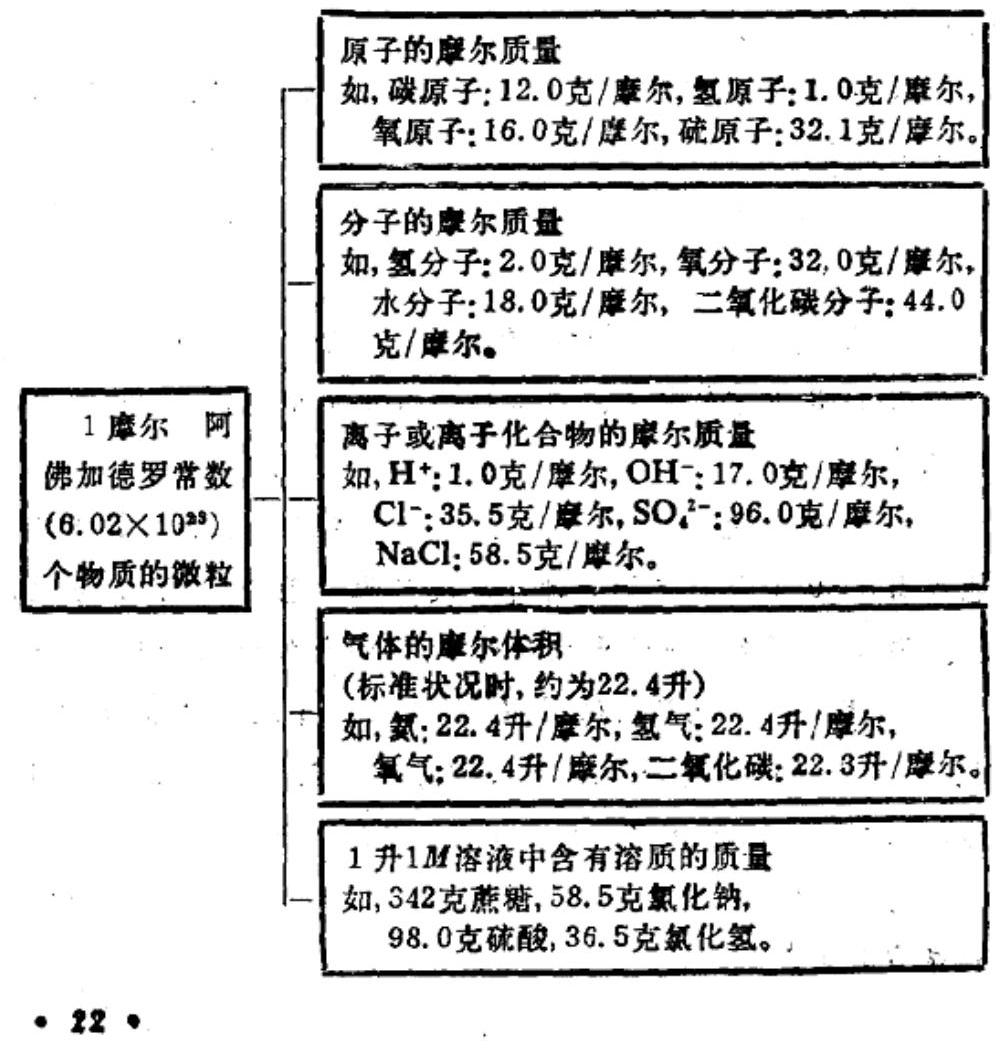
\includegraphics[max width=1.0\textwidth]{images/01912d0f-097c-7e75-8f32-4f326cd86c9f_29_101167.jpg}
\end{center}

物质的量 (摩尔) \(= \frac{\text{ 物质的质量 (克) }}{\text{ 物质的摩尔质量 (克/摩尔) }}\)

气体物质的量 (摩尔) \(= \frac{\text{ 气体的体积 (升) (标准状况) }}{\text{ 气体的摩尔体积 (22.4 升/摩尔) }}\)

摩尔浓度 \(\left( M\right) = \frac{\text{ 溶质的量 (摩尔) }}{\text{ 溶液的体积 (升) }}\)

\section*{二、反应热}

1. 热化学方程式: 表明反应所放出或吸收的热量的化学方程式。

2. 燃烧热: 1 摩尔物质在完全燃烧时所放出的热量。燃烧热热量的计算以 1 摩尔反应物 (可燃物) 为单位。

\section*{复习 题}

1. 下列说法是否正确?并说明理由。

(1)同温同压下,相同质量的气体都占有相同的体积。

(2)摩尔浓度是指 1 升水里所含溶质的摩尔数。

(3) 1 摩尔 NaCl 在水里电离后,可以得到 0.5 摩尔 Na* 和 0.5 摩尔 \({\mathrm{{Cl}}}^{ - }\) 。

2. 在标准状况时, 有 11 克二氧化碳、0.5 摩尔氢气、10升氮气。根据上述情况, 回答下列问题。

(1)哪一种物质的质量最大, 哪一种最小?

(2)哪一种物质所含分子数最多, 哪一种最少?

(3)哪一种物质所占体积最大, 哪一种最小?

3. 2 克硫铵肥料跟浓碱液混和加热, 收集到 600 毫升氨 (标准状况)。计算肥料含氮元素的百分比。

4. 浓度为 \({15}\%\) 、密度为 1.2 克/厘米 \({}^{3}\) 的废硫酸 250 毫升 (不含铁化合物或其它酸)跟过量的铁屑充分反应, 计算:

(1)这种废硫酸的摩尔浓度。

(2)制得氢气(标准状况)的体积。

(3)把生成的硫酸亚铁配制成 400 毫升溶液,这溶液的摩尔浓度是多少。

5. 在含有硫酸钠和碳酸钠的溶液里, 加入足量的氯化钡溶液, 生成沉淀 3.5 克。把沉淀另用足量的硝酸溶液处理, 放出 150 毫升二氧化碳气体(标准状况)。计算溶液里含硫酸钠和碳酸钠各多次摩尔。

6. 计算燃烧多少克氢气, 生成液态水放出的热量跟燃烧 1 千克碳, 生成二氧化碳所放出的热量相等。

7. 称取 1.721 克某种硫酸钙的结晶水合物 \({\mathrm{{CaSO}}}_{4} \cdot x{\mathrm{H}}_{2}\mathrm{O}\) , 加热,使它失去全部结晶水。这时候硫酸钙的质量是 1.361 克, 计算所含结晶水数 \(\left( x\right)\) 。

8. 已知 \(\mathrm{{KCl}}\) 在 \({24}^{ \circ }\mathrm{C}\) 时的溶解度是 33.2 克,计算 \({24}^{ \circ }\mathrm{C}\) 时 \(\mathrm{{KCl}}\) 饱和溶液的百分比浓度。这样浓度的 \(\mathrm{{KCl}}\) 溶液密度为 1.16 克/厘米 \({}^{3}\) ,计算它的摩尔浓度。

\section*{第二章 卤 素}

我们在初中化学里, 已经知道氟原子和氯原子的电子层结构, 它们的最外电子层都有 7 个电子。在 107 种元素的原子里, 还有溴、碘、 破的原子结构跟氟和氯相似, 在最外层都有 7 个电子。氟、氯、溴、碘、 碳具有相似的化学性质, 成为一族, 称为卤族元素, 简称卤素。 破在自然界里含量很少。在这章里, 主要介绍氯, 并在认识氯的基础上, 学习氟、滨、碘。

\section*{第一节 氯 气}

\section*{一、氯气的性质}

\begin{center}
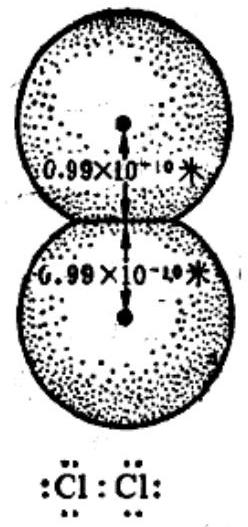
\includegraphics[max width=0.3\textwidth]{images/01912d0f-097c-7e75-8f32-4f326cd86c9f_32_101758.jpg}
\end{center}

图 2-1 氯气分子

氯气 \(\left( {\mathrm{{Cl}}}_{2}\right)\) 的分子是由两个氯原子 \(\Phi\) 组成的双原子分子(图 2-1)。 氯分子也象氢分子一样, 分子里共用电子对处在两个原子核的中间。 氣气是一种非金属单质。在通常情况下, 氯气呈黄绿色, 1 标准大气压下,冷却到 \(- {34.6}^{ \circ }\mathrm{C}\) ,变成液氯、液氯继续冷却到 \(- {101}^{ \circ }\mathrm{C}\) ,变成固态氯。

\customfootnote{

① 氯原子很小, 它的原子半径, 即氯分子中两个原子核间距离的一半,是 \({0.99} \times {10}^{-{10}}\) 米。

}

[实验 2-1] 展示一瓶氯气, 瓶后衬一张白纸, 以便清晰地观察到氯气的颜色。

氯气有毒, 有剧烈的刺激性, 吸入少量氯气会使鼻和喉头的粘膜受到刺激, 引起胸部疼痛和咳嗽; 吸入大量氯气会中毒致死。实验室里; 闻氯气的时候, 必须十分小心, 应该用手轻轻地在瓶口扇动, 仅使极少量的氯气飘进鼻孔 (图 2-2)。

我们已经知道氯原子的最外电子层上有 7 个电子, 因而在化学反应中容易结合一个电子, 使最外电子层达到 8 个电子的稳定结构。氯气的化学性质很活泼, 它是一种活泼的非

金属。

\begin{center}
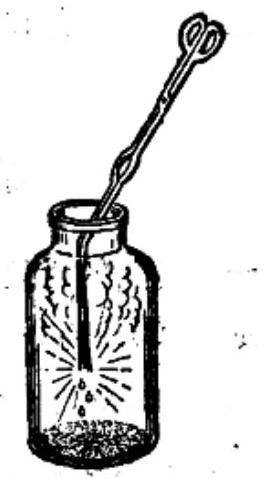
\includegraphics[max width=0.3\textwidth]{images/01912d0f-097c-7e75-8f32-4f326cd86c9f_33_947749.jpg}
\end{center}

\begin{center}
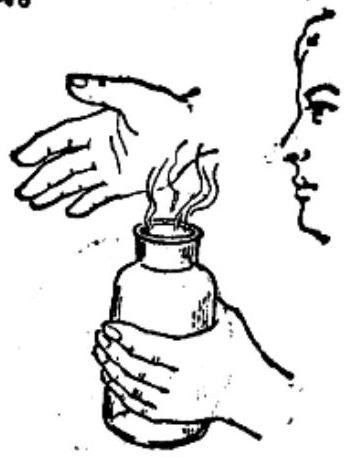
\includegraphics[max width=0.4\textwidth]{images/01912d0f-097c-7e75-8f32-4f326cd86c9f_33_337460.jpg}
\end{center}

图 2-2 闻氣气的方法 图 2-3 铜在氟气里燃烧

\section*{1. 氯气跟金属的反应}

氯气跟金属钠的反应很剧烈, 这在初中化学里已经观察过。氯气不但跟钠等活泼金属直接化合, 而且还能跟受热的铜等某些不活泼的金属起反应。

[实验 2-2] 把一束细铜丝灼热后, 立刻放进盛有氯 气的集气瓶里 (图 2-3), 观察发生的现象。把少量的水注入集气瓶里, 用毛玻璃片把瓶口盖住, 振荡。观察溶液的颜色。

可以看到红热的铜丝在氯气里燃烧起来, 集气瓶里充满棕色的烟, 这是氯化铜晶体颗粒。这个反应可以用化学方程式表示如下:

\[
\mathrm{{Cu}} + {\mathrm{{Cl}}}_{2}\xrightarrow[]{\Delta }{\mathrm{{CuCl}}}_{2}
\]

氯化铜溶解在水里, 成为绿色的氯化铜溶液。

2. 氯气跟非金属的反应

[实验 2-3] 把新收集的一瓶氯气和一瓶氢气 (氢气 和氯气可以分别收集在透明或半透明的塑料制的集气瓶里), 口对口地对着, 抽去瓶口间的较璃片, 上下颠倒几次, 使氯气和氢气充分混和。拿一瓶氣、氢混和气体作试验; 用塑; 料片盖好, 在离瓶约 10 厘米处点燃镁条, 当发生的强光照射混和气体时, 可以观察到因瓶里的氟气眼氢气迅速化合而发生的爆炸, 把塑料片向上弹起 (图2-4)。

\begin{center}
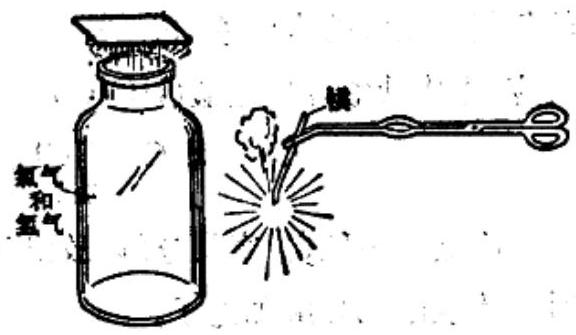
\includegraphics[max width=0.6\textwidth]{images/01912d0f-097c-7e75-8f32-4f326cd86c9f_34_366956.jpg}
\end{center}

图 2-4 氟气跟氢气化合

\begin{center}
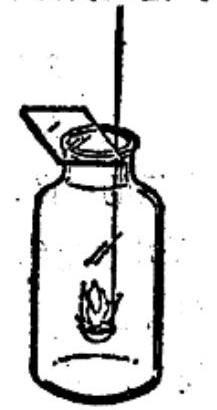
\includegraphics[max width=0.2\textwidth]{images/01912d0f-097c-7e75-8f32-4f326cd86c9f_34_152173.jpg}
\end{center}

氯气跟氢气起反应, 生成氯化氢气体, 放出大量的热, 以致发生爆炸。

\({\mathrm{H}}_{2}\left( \text{ 气 }\right) + {\mathrm{{Cl}}}_{2}\left( \text{ 气 }\right) \frac{\text{ 光照 }}{}2\mathrm{{HCl}}\left( \text{ 气 }\right) + {44.1}\) 千卡

[实验 2-4] 把红磷放在燃烧匙里, 点

燃后插入盛有氯气的集气瓶里, 磷就燃烧起 图 2-5 磷在氯气来(图2-5)。观察发生的现象。 里燃烧

氯气跟磷起反应, 生成三氯化磷和五氯化磷。出现的白色烟雾是三氯化磷和五氯化磷的混和物。

\[
2\mathrm{P} + 3{\mathrm{{Cl}}}_{2}\xrightarrow[]{\text{ 点燃 }}2{\mathrm{{PCl}}}_{3}
\]

\[
{\mathrm{{PCl}}}_{3} + {\mathrm{{Cl}}}_{2} = {\mathrm{{PCl}}}_{5}
\]

\[
\text{五氟化碘}
\]

三氯化磷是无色液体, 是重要的化工原料, 用来制造许多磷的化合物, 如敌百虫等多种农药。

\section*{3. 氯气跟水的反应}

氯气溶解于水, 在常温下, 1 体积的水能够溶解约 2 体积的氯气。氯气的水溶液叫做 “氯水”。溶解的氯气能够跟水起反应, 生成盐酸和次氯酸(HClO)。

\[
{\mathrm{{Cl}}}_{2} + {\mathrm{H}}_{2}\mathrm{O} = \underset{\text{ 盐酸 }}{\mathrm{{HCl}}} + \underset{\text{ 次氯酸 }}{\mathrm{{HClO}}}
\]

次氯酸不稳定, 容易分解, 放出氧气。当氯水受自光照射时, 次氯酸的分解加速子.

[实验 2-5] 当日光照射到如图 2-6 盛有氟水的装置时, 不久就见到有气泡逸出。

\[
2\mathrm{{HClO}}\xrightarrow[]{\text{ 光照 }}2\mathrm{{HCl}} + {\mathrm{O}}_{2} \uparrow
\]

\begin{center}
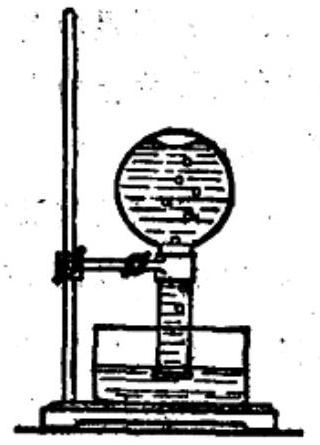
\includegraphics[max width=0.4\textwidth]{images/01912d0f-097c-7e75-8f32-4f326cd86c9f_35_618497.jpg}
\end{center}

次氯酸是一种强氧化剂, 能杀死水里的病菌,所以自来水常用氯气 (1 升水里约通入 0.002 克氯气) 来杀菌消毒。 次氯酸能使染料和有机色质褪色, 可用作漂白剂。

[实验 2-6] 取干燥的和湿润的有 图 2-6 氯水被分解色布条各一条, 放在如图 2-7 的装置里, 观察发生的现象。

可以看到湿润的有色布条褪了色,干燥的却没有(图 2-7)。可见起漂白作用的是次氯酸。

\begin{center}
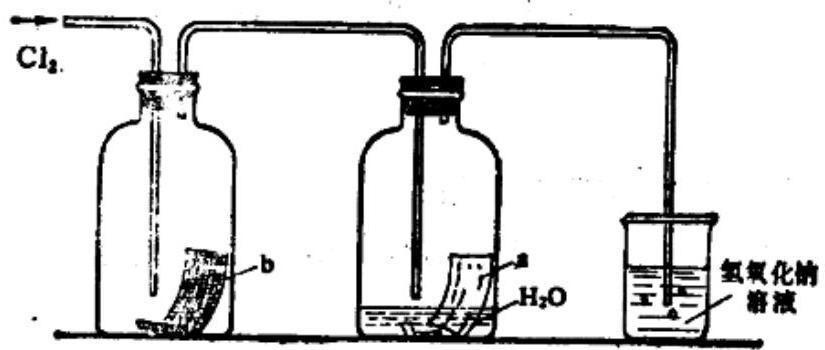
\includegraphics[max width=0.9\textwidth]{images/01912d0f-097c-7e75-8f32-4f326cd86c9f_36_305019.jpg}
\end{center}

图 2-7 次氯酸使色布褪色

\(a\) : 湿润的有色布条 \(b\) : 干燥的有色布条

\section*{4. 氯气跟碱的反应}

氯气跟氢氧化钠等碱类都能较快地发生反应, 所以制氯气时可以用碱液吸收剩余的氯气。

\[
2\mathrm{{NaOH}} + {\mathrm{{Cl}}}_{2} = \mathrm{{NaCl}} + \mathrm{{NaClO}} + {\mathrm{H}}_{2}\mathrm{O}
\]

次氯酸钠

由于次氯酸盐比次氯酸稳定, 容易保存。工业上就用氯气和消石灰制成漂白粉, 漂白粉的冇效成分是次氯酸钙。制漂白粉的反应可以用化学方程式简单表示如下:

\[
2\mathrm{{Ca}}{\left( \mathrm{{OH}}\right) }_{2} + 2{\mathrm{{Cl}}}_{2} = \mathrm{{Ca}}{\left( \mathrm{{ClO}}\right) }_{2} + {\mathrm{{CaCl}}}_{2} + 2{\mathrm{H}}_{2}\mathrm{O}
\]

\[
\text{次氯酸钙}
\]

漂白粉应用于漂白的时候, 使次氯酸钙跟稀酸或空气里的二氧化碳和水蒸气起反应, 就生成次氯酸。

\[
\mathrm{{Ca}}{\left( \mathrm{{ClO}}\right) }_{2} + 2\mathrm{{HCl}} = {\mathrm{{CaCl}}}_{2} + 2\mathrm{{HClO}}
\]

氯化钙

\[
\mathrm{{Ca}}{\left( \mathrm{{ClO}}\right) }_{2} + {\mathrm{{CO}}}_{2} + {\mathrm{H}}_{2}\mathrm{O} = {\mathrm{{CaCO}}}_{3} \downarrow + 2\mathrm{{HClO}}
\]

碳酸钙

\section*{二、氯气的用途}

氯气除用于消毒、制造盐酸和漂白粉外, 还用于制造多种农药,制造氯仿等有机溶剂,所以氯气是一种重要的化工原料。

\section*{三、氯气的实验室制法}

在实验室里, 氯气可以用浓盐酸跟二氧化锰起反应来制取。

[实验 2-7] 象图 2-8 所示那样把装置连接好, 检查气密性。在烧瓶里加入少量二氧化锰粉末, 从分液漏斗慢慢地注入密度为 1.19 克/厘米 \({}^{8}\) 的浓盐酸。缓缓加热,使反应加速, 氯气就均匀地放出。用向上排空气法收集, 多余的氧气用氢氧化钠吸收。

\begin{center}
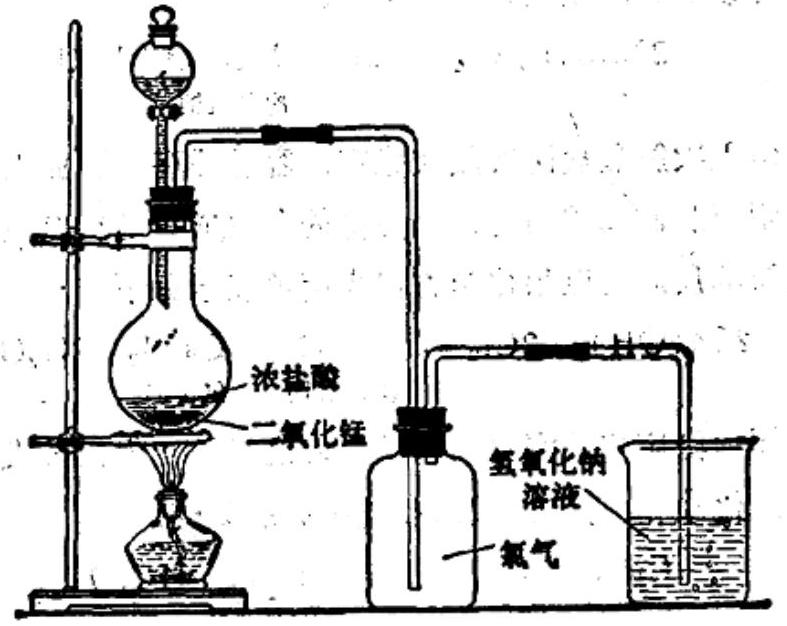
\includegraphics[max width=0.9\textwidth]{images/01912d0f-097c-7e75-8f32-4f326cd86c9f_37_119423.jpg}
\end{center}

图 2-8 实验室制取氟气

这个反应可以用化学方程式表示如下:

\begin{center}
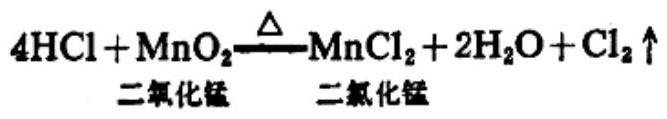
\includegraphics[max width=0.7\textwidth]{images/01912d0f-097c-7e75-8f32-4f326cd86c9f_38_438218.jpg}
\end{center}

\section*{习 题}

1. 下列说法里哪一条是正确的?

(1)戴原子跟氯离子的性质是一样的。

(2)氯离子比氯原子多一个电子。

(3)氯离子呈黄绿色。

2. 新制备的氯水和长久搁置的氯水在成分上有什么不同?

3. 写出氯气跟锌、铝、铁反应的化学方程式。

4. 固态的磷跟氯气起反应, 生成 1 摩尔气态三氧化磷, 放出 73.2 千卡的热; 气态三氯化磷再跟氧气起反应,生成 1 摩尔气态五氧化磷, 放出 22.1 千卡的热。写出这两个热化学方程式。

5. 取含 \({78}\% {\mathrm{{MnO}}}_{2}\) 的软锰矿 150 克,跟足量浓盐酸起反应, 可以制得氯气多少克!

\section*{第二节 氯化氢和盐酸}

\section*{一、氯化氢}

[实验 2-8] 把少量食盐放在烧瓶里 (图 2-9)。通过分液漏斗注入浓硫酸, 同时加热。把氯化氢收集在干燥的容器里。 一部分氯化氢用水收集。

\begin{center}
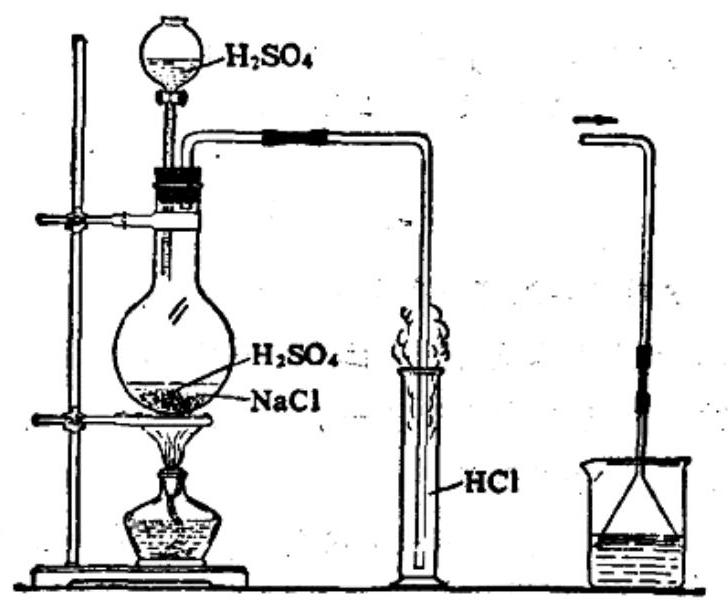
\includegraphics[max width=0.8\textwidth]{images/01912d0f-097c-7e75-8f32-4f326cd86c9f_39_941677.jpg}
\end{center}

图 2-9 实验室制取氯化氢

食盐跟浓硫酸起反应, 不加热或稍微加热, 就生成硫酸氢钠和氯化氢。

\[
\mathrm{{NaCl}} + {\mathrm{H}}_{2}{\mathrm{{SO}}}_{4}\left( \text{ 浓 }\right) = \underset{\text{ 硫酸氢钠 }}{{\mathrm{{NaHSO}}}_{4} + \mathrm{{HCl}} \uparrow }
\]

在 \({500} - {600}^{ \circ }\mathrm{C}\) 的条件下、继续起反应而生成硫酸钠和氯化氢。

\[
{\mathrm{{NaHSO}}}_{4} + \mathrm{{NaCl}} = {\mathrm{{Na}}}_{2}{\mathrm{{SO}}}_{4} + \mathrm{{HCl}} \uparrow
\]

\[
\text{硫酸钠}
\]

总的化学方程式可以表示如下:

\[
2\mathrm{{NaCl}} + {\mathrm{H}}_{2}{\mathrm{{SO}}}_{4}\overset{\bigtriangleup }{ = }{\mathrm{{Na}}}_{2}{\mathrm{{SO}}}_{4} + 2\mathrm{{HCl}} \uparrow
\]

氯化氢是没有颜色而有刺激性的气体。它易溶于水, 在 \({0}^{ \circ }\mathrm{C}\) 时,1 体积的水大约能溶解 500 体积的氯化氢。

[实验 2-9] 在干燥的圆底烧瓶里装满氯化氢, 用带有玻璃管和滴管 (滴管里预先吸入水) 的塞子塞紧瓶口。立即倒置烧瓶, 使玻璃管放进盛着石蕊溶液的烧杯里。压缩滴管的胶头, 出水几滴。烧杯里的溶液即由玻璃管喷入烧瓶, 形成美丽的喷泉(图 2-10)。

\begin{center}
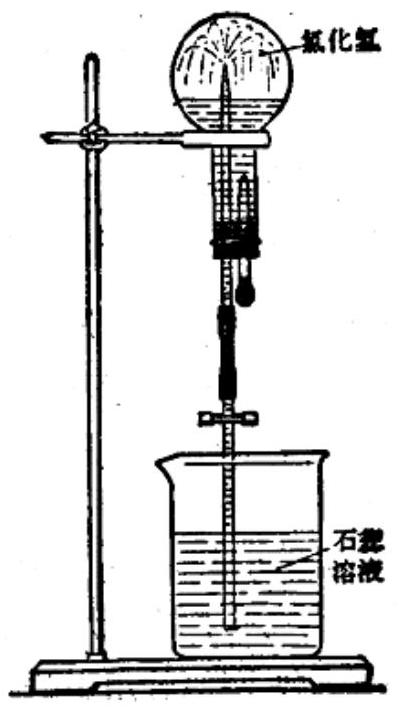
\includegraphics[max width=0.4\textwidth]{images/01912d0f-097c-7e75-8f32-4f326cd86c9f_40_464001.jpg}
\end{center}

\section*{二、盐酸和金属氯化物}

氯化氢的水溶液呈酸性, 叫氢氯酸, 习惯上又叫盐酸。盐酸的性质我们在初中化学里已经学过, 它能够使酸碱指示剂变色, 能够跟金属活动性顺序中氢以前的金属起置换反应, 能够跟碱起中和反应, 能够跟

盐起复分解反应而生成不溶性 图 2-10 氯化氢在水里的溶解的或挥发性的物质。它跟金属、碱或盐反应, 生成金属氯化物。

金属氯化物在自然界里分布很广, 也广泛地应用于日常生活中、工农业生产上等等。重要的有氯化钠、氯化钾、氯化镁、氯化锌等。在这里只介绍氯化钠。

氯化钠俗名食盐, 它对于人和高等动物的正常生理活动是不可缺少的。我们每天要吃一点食盐, 来补充从尿、汗水里所排泄掉的氯化钠。食盐在自然界里分布很广。海水里含有丰富的食盐。由于地壳的变化, 食盐也蕴藏在盐湖、盐井和盐矿中。我国有极为丰富的食盐资源, 盛产海盐、井盐、池盐和岩盐。

海水和盐湖等都蕴藏着丰富的资源。除生产食盐外, 它们的综合利用能够制得钾肥和许多别的盐类, 制得溴等产品。 这些产品是农业和许多工业不可缺少的原料。

从海水晒盐或用从盐井汲出的卤水煮盐, 都是为了把水蒸发掉, 使食盐溶液达到饱和, 继续蒸发, 食盐不断成晶体析出。这样得到的食盐晶体还含有较多的杂质, 常叫粗盐。粗盐经过再结晶, 就得到精盐。

纯净的氯化钠的晶体呈立方形,在 \({801}^{ \circ }\mathrm{C}\) 熔化,在 \({1413}^{ \circ }\mathrm{C}\) 沸腾。纯净的氯化钠在空气里不潮解, 粗盐因含有氯化镁、氯化钙等杂质, 易潮解。

食盐的用途很广。日常生活里用于调味和腌渍蔬菜、鱼肉、蛋类等等。医疗上用的生理盐水是 \({0.9}\%\) 的食盐水。食盐是重要的化工原料, 用于制取金属钠、氯气、氢氧化钠、纯碱等等化工产品。

\section*{习 题}

1. 11.2 升氧气和 11.2 升氢气起反应,生成多少升的 氯化氢气体(气体体积都按标准状况计),把生成的氧化氢都溶解在 328.5 克水里形成密度为 1.047 克/厘米 \({}^{8}\) 的盐酸, 计算这种盐酸的摩尔浓度。

2. 写出盐酸跟下列物质起反应的化学方程式。

\[
\mathrm{{Mg}}\text{、}\mathrm{{MgO}}\text{、}\mathrm{{Mg}}{\left( \mathrm{{OH}}\right) }_{2}\text{、}\mathrm{{Mg}}{\left( {\mathrm{{HCO}}}_{3}\right) }_{2}\text{、}{\mathrm{{MgCO}}}_{3}\text{。}
\]

3. 11.7 克氯化钠跟 10 克浓度为 \({98}\%\) 的硫酸反应, 微热时生成多少克氟化氢? 继续加热到 \({600}^{ \circ }\mathrm{C}\) 时,又生成多少克的氧化氢?

4. 1 克的锌和 1 克的铁分别跟足量的稀盐酸起反应, 各生成多少升的氢气(在标准状况下)?

5. 1.5 毫升密度为 1.028 克/厘米 \({}^{3}\) 的盐酸 \(\left( {6\% \mathrm{{HCl}}}\right)\) 跟足量的硝酸银溶液起反应, 计算生成的氯化银的质量。

6. 为什么在晒盐的时候, 日晒风吹都有利于食盐晶体的析出?

7. 为什么制食盐的时候, 不宜采用降低溶液温度的方法?

\section*{第三节 氧化-还原反应}

我们在初中化学里, 已经学习过氧化-还原反应, 知道氧化、还原并不限于得氧或失氧的反应, 而是可以用正负化合价升降的观点来分析氧化-还原反应。在反应过程里, 物质所含元素化合价升高的反应是氧化反应; 物质所含元素化合价降低的反应是还原反应。所含元素化合价升高的物质是还原剂, 所含元素化合价降低的物质是氧化剂。我们现在就用这个观点来分析在这章里学过的几个氧化-还原反应。

\begin{center}
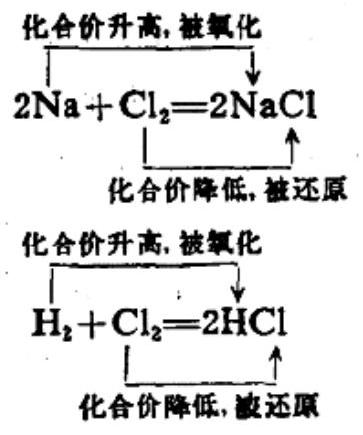
\includegraphics[max width=0.4\textwidth]{images/01912d0f-097c-7e75-8f32-4f326cd86c9f_42_511225.jpg}
\end{center}

我们在初中化学里已经知道, 氯化钠是由氯离子和钠离子构成的。钠原子失去 1 个电子, 成为钠离子, 氯原子得到 1 个电子, 成为氯离子。在这里, 可以从电子得失的观点进一步分析几个氧化-还原反应。

我们知道, 氯气跟钠或铜起反应, 分别生成了氯化钠和氯化铜。在反应过程里,铜原子也象钠原子一样失去了电子成为铜离子。在下面的化学方程式里, “e” 表示电子, 并用箭头表明同一元素的原子得到或失去电子的情况。

\begin{center}
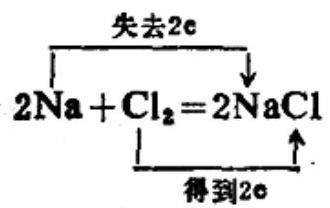
\includegraphics[max width=0.4\textwidth]{images/01912d0f-097c-7e75-8f32-4f326cd86c9f_43_984832.jpg}
\end{center}

\begin{center}
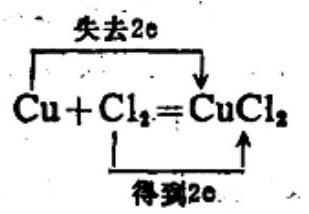
\includegraphics[max width=0.3\textwidth]{images/01912d0f-097c-7e75-8f32-4f326cd86c9f_43_517260.jpg}
\end{center}

\(\mathrm{{NaCl}}\) 里,钠是 +1 价,氯是 -1 价。在反应过程里,钠原子失去 1 个电子, 钠从 0 价变到 +1 价, 化合价升高; 氯原子得到 1 个电子, 氟从 0 价变到 -1 价, 化合价降低。同样地, 铜原子失去 2 个电子, 铜从 0 价升高到 +2 价, 化合价升高; 氯原子得到 1 个电子, 氯从 0 价降低到 -1 价, 化合价降低。 元素化合价升高是由于失去电子, 升高的价数也就是失去的电子数。元素化合价降低是由于得到电子, 降低的价数也就是得到的电子数。元素的化合价升降的原因就是它们的原子失去或得到电子的缘故。所以, 我们可以给氧化-还原反应下一个更确切的定义。

物质失去电子的反应就是氧化反应, 物质得到电子的反应就是还原反应。

在氧化-还原反应里, 一种物质失去电子, 必然同时有别的物质得到电子; 一种物质失去电子的数目总是跟别的物质得到电子的数目相等。得到电子的物质是氧化剂, 失去电子的物质是还原剂。

在下面的化学方程式里, 用箭头表示不同元素间电子得失的情况。

\begin{center}
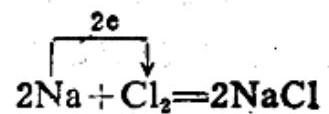
\includegraphics[max width=0.4\textwidth]{images/01912d0f-097c-7e75-8f32-4f326cd86c9f_44_117063.jpg}
\end{center}

还原剂 氧化剂

\begin{center}
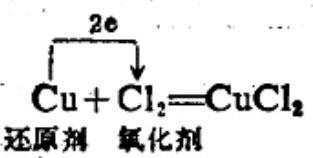
\includegraphics[max width=0.3\textwidth]{images/01912d0f-097c-7e75-8f32-4f326cd86c9f_44_999338.jpg}
\end{center}

但是, 也有一些反应, 如上面讲到的氢气跟氢气生成氯化氢的反应, 生成的氯化氢是共价化合物。我们在初中化学里已经知道, 氯化氢分子里的共用电子对是偏向于氯原子, 偏离于氢原子的。

\[
\text{H}\because \mathrm{{Cl}}\text{:}
\]

在上述电子转移过程里, 就没有那么显著, 也就是并没有完全失去或完全得到电子, 而是共用电子对的偏移。这样的反应也属于氧化-还原反应。在这个反应里, 氯气是氧化剂, 氢气是还原剂。

氧化-还原反应里, 电子转移 (得失或偏移)、正负化合价升降的关系, 可以用图 2-11 表示。 \(- 4 - 3 - 2 - 1\;0 + 1 + 2 + 3 + 4 + 5 + 6 + 7\) 电话:133号

图 2-11 氧化-还原反应中电子得失、化合价变化的关系简图

【例题】分析镁跟稀盐酸的反应里镁元素和氢元素在反应前后的电子得失、化合价升降和氧化、还原的关系。哪一种物质是氧化剂, 哪一种物质是还原剂?

[解] 写出反应的化学方程式, 并用箭头表示镁元素和氢元素在反应前后的电子得失等。

\begin{center}
	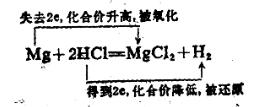
\includegraphics[max width=0.3\textwidth]{images/01912d0f-097c-7e75-8f32-4f326cd86c9f_44_999339.jpg}
\end{center}

答: \(\mathrm{{Mg}}\) 是还原剂, \(\mathrm{{HCl}}\) 是氧化剂。

根据对许多例子的分析, 可以说凡是没有电子转移、也就是没有正负化合价升降的反应, 就不属于氧化-还原反应。

在工农业生产、科学技术和日常生活里, 我们经常会碰到许多氧化-还原反应。所以氧化-还原反应是很重要的一类化学反应。

\section*{习 题}

1. 说明在下列反应里的氧化、还原、化合价升降的关系。

(1) \(2\mathrm{P} + 3{\mathrm{{Cl}}}_{2} = 2{\mathrm{{PCl}}}_{3}\)

(2) \(\mathrm{C} + {\mathrm{O}}_{2} = {\mathrm{{CO}}}_{2}\) The result is the result of the magnetic field is not in the convex component of the convex convex component is not converged to the convex convex convex to the convex convex convex.

(3) \(2\mathrm{{Sb}} + 5{\mathrm{{Cl}}}_{2} = 2{\mathrm{{SbCl}}}_{5}\)

(4) \(2{\mathrm{{KClO}}}_{3} = 2\mathrm{{KCl}} + 3{\mathrm{O}}_{2}\)

2. 你怎样理解氧化-还原反应跟电子得失的关系?举例说明。

3. 分析下列化学反应中化合价变化的关系, 由此说明反应中的电子得失。

(1) \(2\mathrm{{Mg}} + {\mathrm{O}}_{2} = 2\mathrm{{MgO}}\)

(2) \(\mathrm{{Zn}} + 2\mathrm{{HCl}} = {\mathrm{{ZnCl}}}_{2} + {\mathrm{H}}_{2} \uparrow\)

4. 分析下列氧化-还原反应里电子的转移情况, 哪种物质是氧化剂, 哪种物质是还原剂?

(1) \(\mathrm{{Zn}} + {\mathrm{H}}_{2}{\mathrm{{SO}}}_{4} = {\mathrm{{ZnSO}}}_{4} + {\mathrm{H}}_{2} \uparrow\)

(2) \(\mathrm{{Fe}} + 2\mathrm{{HCl}} = {\mathrm{{FeCl}}}_{2} + {\mathrm{H}}_{2} \uparrow\)

5. 写出氯气分别跟钾、钙起反应的化学方程式。在各个反应里分别指出不同元素间电子转移的关系。在各个反应里, 哪种物质是氧化剂, 哪种物质是还原剂?

\section*{第四节 卤 族 元 素}

我们已经学过氯元素的单质和一些重要的化合物。现在学习氟、溴、碘等元素, 并把它们跟氯元素相比较, 它们在性质上、原子结构上有哪些相似和不同的地方。

\section*{一、卤素的原子结构和它们的单质的物理性质}

卤素在自然界里都以化合态存在,它们的单质可由人工制得。卤素的单质都是双原子的分子。下面列出各元素的原子结构和单质的物理性质。

从表 2-1 可以看出, 氟、氯、溴、碘的原子的最外电子层的电子数是相同的, 都是 7 个电子, 但电子层数不同。因此, 它们的原子半径或离子半径 \(\Phi\) 都随着电子层数的增多而增大 (图 2-12), 它们的离子都因得到了一个电子, 离子半径比相应的原子半径增大了。

\begin{center}
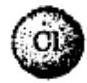
\includegraphics[max width=0.2\textwidth]{images/01912d0f-097c-7e75-8f32-4f326cd86c9f_47_783842.jpg}
\end{center}

\begin{center}
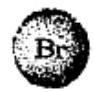
\includegraphics[max width=0.2\textwidth]{images/01912d0f-097c-7e75-8f32-4f326cd86c9f_47_196612.jpg}
\end{center}

\begin{center}
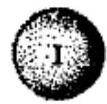
\includegraphics[max width=0.2\textwidth]{images/01912d0f-097c-7e75-8f32-4f326cd86c9f_47_881999.jpg}
\end{center}

1.14 1.33

\begin{center}
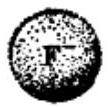
\includegraphics[max width=0.2\textwidth]{images/01912d0f-097c-7e75-8f32-4f326cd86c9f_47_511057.jpg}
\end{center}

\begin{center}
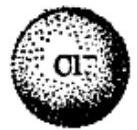
\includegraphics[max width=0.2\textwidth]{images/01912d0f-097c-7e75-8f32-4f326cd86c9f_47_995315.jpg}
\end{center}

\begin{center}
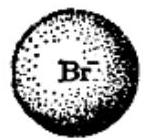
\includegraphics[max width=0.2\textwidth]{images/01912d0f-097c-7e75-8f32-4f326cd86c9f_47_752852.jpg}
\end{center}

\begin{center}
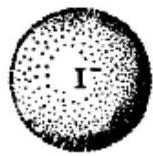
\includegraphics[max width=0.2\textwidth]{images/01912d0f-097c-7e75-8f32-4f326cd86c9f_47_891413.jpg}
\end{center}

1.33 1.81 1.96 2.20

图 2-12 卤素的原子和离子大小示意图 (数据单位是 \({10}^{-{10}}\) 米)

从表 2-1 还可以看出, 卤素的物理性质有较大的差别。如在常温, 氟、氯是气体, 溴是液体, 碘是固体, 它们的沸点、熔点都逐渐升高, 颜色由淡黄绿色到紫黑色, 逐渐转深。

[实验 2-10] 打开盛溴的瓶的盖子, 有什么现象发生! 观察液态和气态的溴。

可以观察到, 液态溴容易挥发成溴蒸气。

[实验 2-11] 观察碘的颜色、状态和光泽。把少量的碘晶体放在烧杯里,烧杯上放盛冷水的烧瓶,稍稍加热(图 2-13)。观察发生的现象。

\customfootnote{

① 离子半径是根据阴阳离子的核间距离推算出来的。阴离子的半径比它们的原子半径大, 阳离子的半径比它们的原子半径小。

}

破孙鞋啉邬盛寅哇妹窦士惠明洋甲 I-Z

\begin{center}
\adjustbox{max width=\textwidth}{
\begin{tabular}{|c|c|c|c|c|}
\hline
出装 .(水平 OOI) & 图凶 & s米面 9ZZ & 4,171 & \({26}{60}^{ \circ }0\) \\
\hline
点C & 2.19 & -10 & 1.27 & 1.56 \\
\hline
点CO & -168,848 & 一华 & 587,783 & 134,344 \\
\hline
侧卸 & 长/华69* I & 女/孕 DIS'S & :米圖/軍6II'8 & :米爾/亞 86*t \\
\hline
浮升张司溪 & 判与因割系系 & 书与司對專 & 判職司工業並 & 水园母蛋清 \\
\hline
单质 & F & d. & B & L \\
\hline
鸣小母实断 & ) ) & ) 】8 ) & ) ) 】 ) & 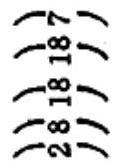
\includegraphics[max width=0.2\textwidth]{images/01912d0f-097c-7e75-8f32-4f326cd86c9f_48_994676.jpg} \\
\hline
核电荷数 & 。 & 17 & 355 & 53 \\
\hline
元素符号 & FL & a & B & 1 \\
\hline
元素名称 & 氟 & 氯 & 溴 & 碘 \\
\hline
\end{tabular}
}
\end{center}

。盛濠朝和园米里香源烤箱酒墨‘我

可以观察到, 碘在常压下加热, 不经过熔化就直接变成紫色蒸气, 蒸气遇冷, 重新凝成固体。这种固态物质不经过转变成液态而直接变成气态的现象叫做升华。

\begin{center}
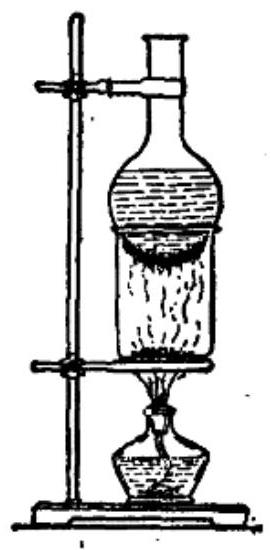
\includegraphics[max width=0.3\textwidth]{images/01912d0f-097c-7e75-8f32-4f326cd86c9f_49_731413.jpg}
\end{center}

图 2-13 碘的升华

\begin{center}
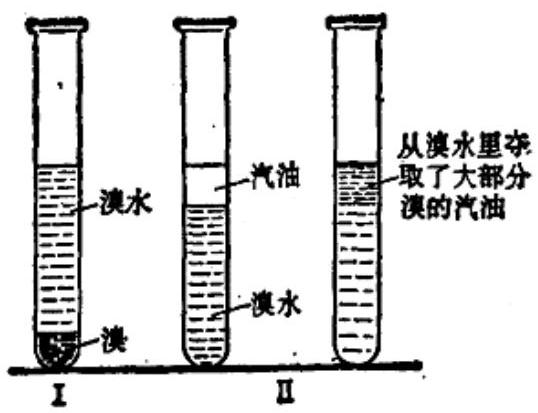
\includegraphics[max width=0.6\textwidth]{images/01912d0f-097c-7e75-8f32-4f326cd86c9f_49_749414.jpg}
\end{center}

图 2-14 溴在不同溶剂里的溶解

[实验 2-12] 把水注入盛着少量溴的试管, 振荡, 水溶液的颜色显橙色 (图 2-14, I)。把上部橙色溶液倒在另一个试管里, 再注入少量无色的汽油 (或苯或四氯化碳) (图 2-14, II), 用力振荡, 静置一会儿。观察油层和水溶液的颜色。

[实验 2-13] 把水、酒精分别注入两个试管, 各约占小半试管, 并各投入少量的碘的晶体, 振荡。比较碘在两种液体里的溶解性。把碘的水溶液注入另一空试管, 再注入少量无色汽油 (或苯或四氯化碳), 振荡, 静置一会儿, 观察油层和溶液的颜色。

可以观察到溴和碘都比较容易溶解于汽油、苯、四氯化碳、酒精等有机溶剂中。医疗上用的碘酒, 即是碘的酒精溶液。

\section*{二、卤素的单质的化学性质}

我们知道, 氯的化学性质很活泼, 它的原子的最外电子层是 7 个电子, 在化学反应中容易得到一个电子而成为 8 个电子的稳定结构。氟、溴、碘的原子的最外电子层也都是 7 个电子, 因而它们的化学性质跟氯有很大的相似性。

\section*{1. 卤素都能跟金属起反应生成卤化物}

[实验 2-14] 在 1 个铁坩埚里放锌粉 0.5 克, 加入碘粉 0.5 克, 混和后, 加水 1-2 滴作为催化剂, 观察发生的现象。

氟、溴、碘都能象氯一样跟钠等金属起反应。自然界里, 也存在着许多种的金属跟卤素的化合物, 如氟化钙、氯化钠、 氯化镁、溴化钾、碘化钾等等卤化物。

\section*{2. 卤素都能跟氢气起反应, 生成卤化氢}

氟的性质比氯更活泼, 氟气跟氢气的反应不需光照, 在暗处就能剧烈化合, 并发生爆炸。

\[
{\mathrm{H}}_{2}\left( \text{ 气 }\right) + {\mathrm{F}}_{2}\left( \text{ 气 }\right) = 2\mathrm{{HF}}\left( \text{ 气 }\right) + {128.4}\text{ 千卡 }
\]

氟化氫

溴的性质不如氯活泼,溴跟氢气的反应在达到 \({500}^{ \circ }\mathrm{C}\) 时即较慢地进行。

\[
{\mathrm{H}}_{2}\left( \text{ 气 }\right) + {\mathrm{{Br}}}_{2}\left( \text{ 气 }\right) = 2\mathrm{{HBr}}\left( \text{ 气 }\right) + {17.3}\text{ 千卡 }
\]

澳化氢

碘的性质比溴更不活泼, 碘跟氢气的反应在不断加热条件下缓慢地进行, 生成的碘化氢很不稳定, 同时发生分解。

\[
{\mathrm{H}}_{2}\left( \text{ 气 }\right) + {\mathrm{I}}_{2}\text{ (固) } = 2\mathrm{{HI}}\left( \text{ 气 }\right) - {12.4}\text{ 千卡 }
\]

卤素也能跟磷等非金属起反应。

3. 卤素跟水的反应

氟遇水发生剧烈的反应, 生成氟化氢和氧气。

\[
2{\mathrm{H}}_{2}\mathrm{O} + 2{\mathrm{\;F}}_{2} = 4\mathrm{{HF}} + {\mathrm{O}}_{2} \uparrow
\]

溴跟水的反应比氯气跟水的反应更弱一些, 碘跟水只有很微弱的反应。

\section*{4. 卤素各单质的活动性比较}

[实验 2-15] 把少量氯水分别注入盛着溴化钠溶液和碘化钾溶液的两个试管里, 用力振荡后, 再注入少量无色汽油 (或四氯化碳)。振荡。观察油层和溶液颜色的变化。

[实验 2-16] 把少量溴水注入盛着碘化钾溶液的试管里, 用力振荡。观察溶液颜色的变化。

溶液颜色的变化,说明氯可以把溴或碘从它们的化合物里置换出来, 溴可以把碘从它的化合物中置换出来。

\[
2\mathrm{{NaBr}} + {\mathrm{{Cl}}}_{2} = 2\mathrm{{NaCl}} + {\mathrm{{Br}}}_{2}
\]

\[
2\mathrm{{KI}} + {\mathrm{{Cl}}}_{2} = 2\mathrm{{KCl}} + {\mathrm{I}}_{2}
\]

\[
2\mathrm{{KI}} + {\mathrm{{Br}}}_{2} = 2\mathrm{{KBr}} + {\mathrm{I}}_{2}
\]

由此可以证明, 在氯、溴、碘这三种元素里, 氯比溴活泼, 溴又比碘活泼。实验证明, 氟的性质比氯、溴、碘更活泼, 能把氯等从它们的卤化物中置换出来。

氟的性质特别活泼, 它甚至还能够跟惰性气体中的氙、氪等起反应,生成氙和氪的氟化物 \(\Phi : {\mathrm{{XeF}}}_{2}\text{、}{\mathrm{{XeF}}}_{4}\text{、}{\mathrm{{XeF}}}_{8}\text{、}{\mathrm{{KrF}}}_{2}\) 等。它们在常温下都是白色固体。

\section*{5. 碘跟淀粉的反应}

碘遇淀粉变蓝色。利用碘的这个特性, 可以鉴定碘的存在。

\customfootnote{

\({\text{①}}^{ \circ }\) 氙和氪的氟化物的结构比较特殊,不宜应用通常的正负化合价来解释。

}

[实验 2-17] 在试管里注入少量淀粉溶液, 滴入几滴碘水, 溶液显示出特殊的蓝色。

从卤素的化学性质可以看出, 它们有很多相似的地方, 但也有差别 (表 2-2)。卤素的原子, 最外电子层都有 7 个电子,

表 2-2 卤素的单质的化学性质比较

\begin{center}
\adjustbox{max width=\textwidth}{
\begin{tabular}{|c|c|c|c|}
\hline
分子式 & 跟氢气的反应和 氢化物的稳定性 & 跟水的反应 & 卤素的活动性比较 \\
\hline
\({\mathrm{F}}_{2}\) & 在冷暗处就能剧烈 化合而爆炸, HF 很 稳定。 & 使水迅速分解, 放出氧气。 & 氟最活泼, 能把氯、 溴、碘从它们的化 合物中置换出来。 \\
\hline
\({\mathrm{{Cl}}}_{2}\) & 在强光照射下, 剧烈 化合而爆炸, \(\mathrm{{HCl}}\) 较 稳定。 & 在日光照射下, 缓慢放出氧气。 & 氣次之,能把溴、碘 从它们的化合物中 置换出来。 \\
\hline
\({\mathrm{{Br}}}_{2}\) & 在高温条件下, 较慢 地化合, \(\mathrm{{HBr}}\) 较不稳 定。 & 反应较氯为弱。 & 溴又次之,能把碘 从它的化合物中置 换出来。 \\
\hline
1, & 持续加热, 慢慢地化 合, \(\mathrm{{HI}}\) 很不稳定, 同 时发生分解。 & 只起很微弱的 反应。 & 碘较不活泼。 \\
\hline
\end{tabular}
}
\end{center}

结合外来电子的能力很强, 所以卤素是活泼的非金属元素。卤素容易得到电子而被还原, 它们本身是强氧化剂。但是, 氟、 氯、溴、碘各原子的核电荷数不同、核外电子层数不同, 原子和离子的大小也都不同, 各原子核对外层电子的引力也有所不同。原子的大小对非金属的活动性有很密切的关系。氟的原子较小, 外层电子受到核的引力最强, 它得到电子的能力很强, 非金属性最活泼, 所以合成的氟化氢最稳定, 合成的时候反应放热, 并最剧烈。碘的原子较大, 最外层电子受到核的引力较弱, 它得到电子的能力也较弱, 非金属性也较弱, 生成的碘化氢不稳定, 合成的时候要吸热。氯和溴的非金属性是介乎其间的, 氯比溴又活泼一些。总的看来, 卤素是活泼的非金属元素, 它们的活动性又随着核电荷数和电子层数的增加、原子半径的增大而减弱。

[讨论] 从哪些方面可以比较氟、氯、溴、碘的性质的相似和不同之处?

\section*{三、卤素的几种化合物}

\section*{1. 氟化氢和氟化钙}

氟化钙俗名萤石, 是自然界里存在相当广泛的氟的化合物。

使浓硫酸跟萤石在铅皿中起反应, 就制得氟化氢。

\[
{\mathrm{{CaF}}}_{2} + {\mathrm{H}}_{2}{\mathrm{{SO}}}_{4} = {\mathrm{{CaSO}}}_{4} + 2\mathrm{{HF}} \uparrow
\]

氟化氢也象氯化氢那样, 在空气里呈现白雾。氟化氢有剧毒。氟化氢溶解在水里就是氢氟酸。

氟化氢用于雕刻玻璃和制造塑料、橡胶、药品等, 还用于制备单质氟和提炼铀。氟化氢还用于制造氟化钠等氟化物。 氟化钠是一种用来杀灭地下害虫的农药。

\section*{2. 溴化银和碘化银}

[实验 2-18] 把少量硝酸银溶液分别滴入盛着溴化钠溶液和碘化钾溶液的两个试管。在盛溴化钠溶液的试管里有浅黄色的溴化银沉淀生成, 在盛碘化钾溶液的试管里有黄色的碘化银沉淀生成。在两个试管里各加入少量稀硝酸, 生成的溴化银、碘化银沉淀都不溶解。

\[
\mathrm{{NaBr}} + {\mathrm{{AgNO}}}_{3} = \underset{\text{ 溴化银 }}{\mathrm{{AgBr}} \downarrow } + \underset{\text{ 硝酸钠 }}{{\mathrm{{NaNO}}}_{3}}
\]

\[
\mathrm{{KI}} + {\mathrm{{AgNO}}}_{3} = \underset{\text{ 碘化银 }}{\mathrm{{AgI}} \downarrow } + {\mathrm{{KNO}}}_{3}
\]

溴化银和碘化银都有感光性, 在光的照射下会起分解反应。例如:

\[
2\mathrm{{AgBr}}\xrightarrow[]{\text{ 光照 }}2\mathrm{{Ag}} + {\mathrm{{Br}}}_{2}
\]

照相用的感光片, 就是在暗室里用溴化银的明胶凝胶, 均匀地涂在胶卷或玻璃片上制成的。照相时利用溴化银有感光性的原理, 使底片感光后, 再用还原剂(显影剂) 和定影剂处理, 得到明暗程度跟实物相反的底片。使感光片通过底片曝光, 再经显影和定影, 就得到明暗程度跟实物一致的照片。

碘化银可用于人工降雨, 用小火箭、高射炮等工具把磨成很细粉末的碘化银发射到几千米的高空, 使空气里的水蒸气凝聚成雨。

\section*{习 题}

1. 写出氟、溴、碘跟金属钠的反应的化学方程式。

2. 在三个试管里, 分别或着氯化钠、溴化钠、碘化钾的溶液。各加入一些氯水, 发生什么反应?再加入一些溶剂汽油, 振荡。出现什么现象?

3. 从哪些化学性质可以证明氟是卤素中最活泼的元素?

4. 日光照射在下列物质上, 各有什么现象发生? 为什么? 写出化学方程式。

(1)氯水,(2)氯气和氢气的混和物,(3)溴化银。

5. 怎样鉴别单质碘和碘离子?

6. 现有二氧化锰、氯化钾、溴化钾、浓硫酸和水五种物质, 怎样从这些物质来制取盐酸、氯气和溴。写出反应的化学方程式。

7. 氟化钙跟浓硫酸起反应, 制得氟化氢, 写出反应的化学方程式。为什么这个反应的装置不能用玻璃仪器?

\section*{内容提要}

卤素是一族非金属元素。它们的原子结构的共同之点是最外电子层都有 7 个电子, 在化学反应中容易得到电子; 差别之处是核电荷数不同、电子层数不同, 原子半径也不同, 由此形成了卤族元素既相似又有着差别的性质。它们的化学性质主要是强的非金属性, 它们的单质都是强氧化剂。卤素里, 氟原子很小, 非金属性很强, 氯、溴、碘随着原子的增大而非金属性减弱。

\begin{center}
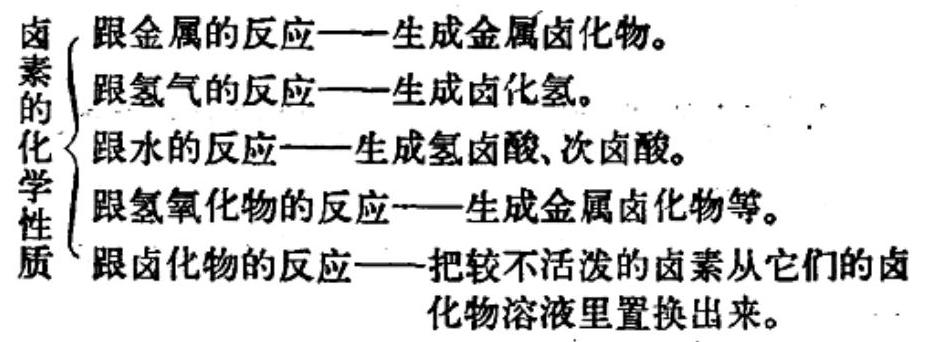
\includegraphics[max width=1.0\textwidth]{images/01912d0f-097c-7e75-8f32-4f326cd86c9f_55_279371.jpg}
\end{center}

物质失去电子的反应是氧化反应, 物质得到电子的反应是还原反应。氧化和还原反应必然同时发生。

\section*{复习 题}

1. 下列说法是否正确, 如不正确, 加以改正。

(1)氯酸钾里有氧气, 所以加热时有氧气放出。

(2)卤素各单质都可以成为氧化剂。

(3)1 摩尔液态 \(\mathrm{{HCl}}\) 在标准状况时约占 22.4 升。

2. 能不能在下列条件下收集氯气? 说明原因, 并写出可能发生的反应的化学方程式。

(1)排水收集,(2)排氢氧化钾溶液收集,(3)排碘化钾溶液收集。

3. 在用氯酸钾制氧气和浓盐酸制氯气时都要用到二氧化锰, 二氧化锰的作用是否相同, 分别是起了什么作用?

4. 实验室里制备氢气、氯气、二氧化碳都要用到盐酸。盐酸在制备这三种气体的反应里, 各起什么作用?

5. 从电子得失的观点来看, 在已经学过的化学反应类型里, 置换反应都属于氧化-还原反应, 一部分化合反应和分解反应属于氧化-还原反应,复分解反应都不属于氧化-还原反应。你认为这个结论合理吗? 举例说明。

6. 一包白色固体,可能是 \({\mathrm{{CaCl}}}_{2}\text{、}{\mathrm{{Na}}}_{2}{\mathrm{{CO}}}_{8}\text{、}\mathrm{{NaI}}\) 三种物质之一,也可能是两者或三者的混和物。当把白色固体溶解于水时,发现有白色沉淀。过滤后,滤液是无色的。

(1)把滤纸上的沉淀, 移到试管里, 加入盐酸, 有气体产生。把气体通入澄清石灰水, 石灰水显浑浊。

(2)把滤液分成两部分。向一部分滤液加入几滴硝酸银溶液, 出现白色沉淀。再加稀硝酸, 白色沉淀不溶解。这白色沉淀光照后,逐渐呈黑色。向另一部分滤液里加几滴氯水, 再注入少许四氯化碳,振荡,四氯化碳层不显紫色。

试分析并判断这包白色固体里含有哪些物质。写出反应的化学方程式。

7. 使足量浓硫酸跟 11.7 克氯化钠混和微热, 反应生成的氧化氢通入 45 克 10\% 氢氧化钠溶液,向最后的溶液滴入几滴石蕊试液, 将显什么颜色。

8. 浓盐酸跟二氧化锰起反应, 生成的氯气能从碘化钠溶液里置换出 1.27 克碘。计算至少需用多少摩尔的 \(\mathrm{{HCl}}\) 和 \({\mathrm{{MnO}}}_{2}\) 。

9. 把滤纸用淀粉和碘化钾的溶液浸泡, 晾干后就是实验室常用的淀粉碘化钾试纸。这种试纸润湿后遇到氯气会发生什么变化? 为什么?

\section*{第三章 硫 硫酸}

硫是一种重要的非金属元素。硫的原子结构和性质跟我们已经学过的氧很相似, 它们的原子的最外电子层都有 6 个电子, 氧 \(\left( \mathrm{O}\right)\) 、硫 \(\left( \mathrm{S}\right)\) 和另外三种原子结构和性质相似的元素硒 (Se)、碲(Te)、钋(Po) \(\Phi\) ,统称为氧族元素。本章主要介绍硫及其化合物的知识。

\section*{第一节 硫}

在自然界, 游离态的天然硫, 存在于火山喷口附近或地壳的岩层里。由于天然硫的存在, 人类从远古时代起就知道硫了。以化合态存在的硫分布很广, 主要是硫化物和硫酸盐, 如硫铁矿 \(\left( {\mathrm{{FeS}}}_{2}\right)\) ,黄铜矿 \(\left( {\mathrm{{CuFeS}}}_{2}\right)\) ,石膏 \(\left( {{\mathrm{{CaSO}}}_{4} \cdot 2{\mathrm{H}}_{2}\mathrm{O}}\right)\) ,芒硝 \(\left( {{\mathrm{{Na}}}_{2}{\mathrm{{SO}}}_{4} \cdot {10}{\mathrm{H}}_{2}\mathrm{O}}\right)\) ,等等。硫的化合物也常存在于火山喷 出的气体中和矿泉水里。煤和石油里都含有少量硫。硫还是某些蛋白质的组成元素, 是生物生长所需要的一种元素。

\section*{一、硫的物理性质}

硫通常是一种淡黄色的晶体, 俗称硫黄。它的密度大约是水的两倍。 硫很脆, 容易研成粉末, 不溶于水, 微溶于酒精, 容易溶于二硫化碳。硫的熔点是 \({112.8}^{ \circ }\mathrm{C}\) ,沸点是 \({444.6}^{ \circ }\mathrm{C}\) 。

\customfootnote{

① 硒音 \(x\mathrm{I}\) ,碲音 \(\mathrm{{di}}\) ,针音 \({\mathrm{p}}_{\mathrm{e}}\)

}

\section*{二、硫的化学性质}

硫的化学性质比较活泼, 跟氧相似, 容易跟金属、氢气和其它非金属发生反应。

\section*{1. 硫跟金属的反应}

[实验 3-1] 给盛着硫粉的大试管加热。加热到硫沸腾产生蒸气时, 用坩埚钳夹住一束擦亮的细铜丝伸入管口(图 3-1), 观察发生的现象。

\begin{center}
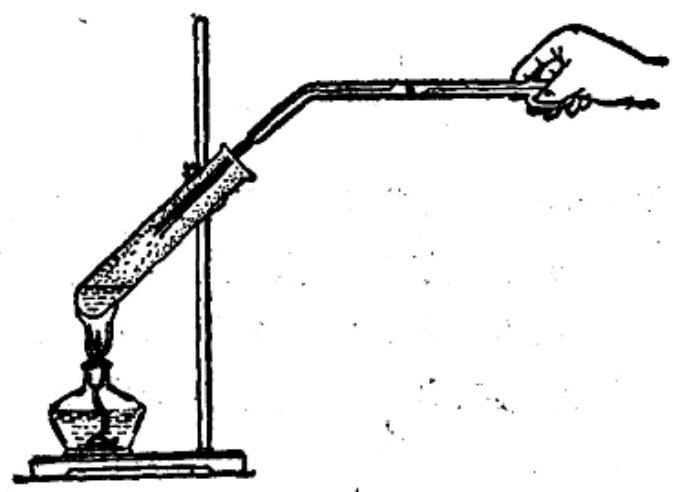
\includegraphics[max width=0.7\textwidth]{images/01912d0f-097c-7e75-8f32-4f326cd86c9f_59_228906.jpg}
\end{center}

图 3-1 铜在硫蒸气里燃烧

铜丝在硫蒸气里燃烧, 生成黑色的硫化亚铜。

\[
2\mathrm{{Cu}} + {\mathrm{S}}^{\Delta } - {\mathrm{{Cu}}}_{2}\mathrm{\;S}
\]

[实验 3-2] 把少量硫粉和铁粉的混和物装在试管里, 加热到红热, 立即把酒精灯移开。反应里放出的热, 就能使反应继续进行。观察发生的现象。

硫跟铁起反应, 生成黑色的硫化亚铁。

\[
\mathrm{{Fe}} + {\mathrm{S}}^{\overset{\bigtriangleup }{ = }}\mathrm{{FeS}}
\]

硫还能跟其它金属起反应。硫跟金属的化合物, 叫做金属硫化物。

\section*{2. 硫跟非金属的反应}

在初中化学里, 我们已经知道硫能跟氧气发生反应, 生成二氧化硫, 并放出大量的热。

\[
\mathrm{S}\left( \text{固}\right) + {\mathrm{O}}_{2}\left( \text{气}\right) = {\mathrm{{SO}}}_{2}\left( \text{气}\right) + {71}\text{千卡}
\]

此外, 硫还能跟其它非金属发生反应。例如, 硫的蒸气能跟氢气直接化合而生成硫化氢气体:

\[
\mathrm{S} + {\mathrm{H}}_{2}\overset{\bigtriangleup }{ = }{\mathrm{H}}_{2}\mathrm{\;S}
\]

\section*{三、硫的用途}

硫的用途很广。硫主要用来制造硫酸。硫也是生产橡胶制品的重要原料。硫还可用于制造黑色火药、焰火、火柴等。 硫又是制造某些农药(如石灰硫黄合剂)的原料。医疗上, 硫还可用来制硫黄软膏医治某些皮肤病, 等等。

\section*{习 题}

1. 写出硫跟氢气、硫跟氧气反应的化学方程式。

2. 试计算 0.32 千克的硫燃烧生成二氧化硫, 放出多少热量。

3. 21 克铁粉跟 8 克硫粉混和加热可生成硫化亚铁多少充, 哪一种物质过剩, 剩余多少?

\section*{第二节 硫的氢化物和氧化物}

\section*{一、硫的氢化物——硫化氢( \({\mathrm{H}}_{2}\mathrm{\;S}\) )}

\section*{1. 硫化氢的实验室制法}

在实验室里, 硫化氢通常是由硫化亚铁跟稀盐酸或稀硫酸反应而制得的。

\[
\mathrm{{FeS}} + 2\mathrm{{HCl}} = {\mathrm{{FeCl}}}_{2} + {\mathrm{H}}_{2}\mathrm{\;S} \uparrow
\]

\[
\mathrm{{FeS}} + {\mathrm{H}}_{2}{\mathrm{{SO}}}_{4} = {\mathrm{{FeSO}}}_{4} + {\mathrm{H}}_{2}\mathrm{\;S} \uparrow
\]

这个反应可以在启普发生器里进行。

\section*{2. 硫化氢的性质}

硫化氢是一种没有颜色而有臭鸡蛋气味的气体。它的密度比空气略大。硫化氢有剧毒, 是一种大气污染物。空气里如果含有微量的硫化氢, 就会使人感到头痛、头晕和恶心。吸入较多的硫化氢, 会使人昏迷甚至死亡。因此, 制取或使用硫化氢时, 必须在密闭系统或通风橱中进行。

硫化氢能溶于水。在常温、常压下, 1体积的水能溶解 2.6 体积的硫化氢。

在较高温度时, 硫化氢分解成氢气和硫。

\[
{\mathrm{H}}_{2}\mathrm{\;S} \triangleq {\mathrm{H}}_{2} + \mathrm{S}
\]

硫化氢是一种可燃性气体。

〔实验 3-3〕 在导管口用火点燃硫化氢气体, 观察硫化氢完全燃烧时火焰的颜色。然后把干燥的烧杯罩在火焰的上方, 观察烧杯内壁附有什么物质。小心地闻一下气味。

在空气充足条件下,硫化氢能完全燃烧而发生淡蓝色的火焰, 并生成水和二氧化硫。

\[
2{\mathrm{H}}_{2}\mathrm{\;S} + 3{\mathrm{O}}_{2}\xrightarrow[]{\text{ 点燃 }}2{\mathrm{H}}_{2}\mathrm{O} + 2{\mathrm{{SO}}}_{2}
\]

[实验 3-4] 在导管口用火点燃硫化氢气体, 用一个 蒸发皿 (或玻璃片), 使蒸发皿底靠近硫化氢的火焰, 观察蒸发皿底发生的现象。

我们可以看到,蒸发皿底部附有黄色的粉末。这是硫化氢不完全燃烧时析出的单质硫。

\[
2{\mathrm{H}}_{2}\mathrm{\;S} + {\mathrm{O}}_{2} = 2{\mathrm{H}}_{2}\mathrm{O} + 2\mathrm{\;S}
\]

如果在一个集气瓶里, 使硫化氢跟二氧化硫两种气体充分混和。不久, 在瓶壁上就有黄色的粉末一一硫的生成。

\[
{\mathrm{{SO}}}_{2} + 2{\mathrm{H}}_{2}\mathrm{\;S} = 2{\mathrm{H}}_{2}\mathrm{O} + 3\mathrm{\;S}
\]

由此可见, 硫化氢具有还原性。硫化氢里的硫是 -2 价, 它能够失去电子而变成游离态的单质硫或高价硫的化合物。

硫化氢的水溶液能够使石蕊试液变为浅红色, 它是一种酸, 叫做氢硫酸, 当这种酸受热时, 硫化氢又从水里逸出。氢硫酸是一种弱酸, 它具有酸的通性。

\section*{二、硫的氧化物}

硫的氧化物中最重要的是二氧化硫和三氧化硫。

1. 二氧化硫 \(\left( {\mathrm{{SO}}}_{2}\right)\)

二氧化硫是没有颜色而有刺激性气味的有毒气体。它的密度比空气大,容易液化 (沸点是 \(- {10}^{ \circ }\mathrm{C}\) ),易溶于水,在常温、 常压下, 1 体积水大约能溶解 40 体积二氧化硫。

二氧化硫是酸性氧化物,它跟水化合而生成亚硫酸 \(\left( {{\mathrm{H}}_{2}{\mathrm{{SO}}}_{3}}\right)\) 。因此,二氧化硫又叫做亚硫酐。

\[
{\mathrm{{SO}}}_{2} + {\mathrm{H}}_{2}\mathrm{O} = {\mathrm{H}}_{2}{\mathrm{{SO}}}_{3}
\]

亚硫酸很不稳定, 容易分解成二氧化硫和水。

\[
{\mathrm{H}}_{2}{\mathrm{{SO}}}_{3} = {\mathrm{H}}_{2}\mathrm{O} + {\mathrm{{SO}}}_{2} \uparrow
\]

通常把向生成物方向进行的反应叫做正反应, 向反应物方向进行的反应叫做逆反应。象这种在同一条件下, 既能向正反应方向进行, 同时又能向逆反应方向进行的反应, 叫做可逆反应。在化学方程式里, 用两个方向相反的箭头代替等号来表示可逆反应。

\[
{\mathrm{{SO}}}_{2} + {\mathrm{H}}_{2}\mathrm{O} \rightleftharpoons {\mathrm{H}}_{2}{\mathrm{{SO}}}_{3}
\]

二氧化硫在适当的温度并有催化剂存在的条件下, 可以被氧气氧化而生成三氧化硫。

\[
2{\mathrm{{SO}}}_{2} + {\mathrm{O}}_{2}\frac{\text{ 催化剂 }}{\bigtriangleup }2{\mathrm{{SO}}}_{3}
\]

[实验 3-5] 把二氧化硫气体通入盛有品红溶液的试 管里, 观察品红溶液颜色的变化。把试管加热, 再观察溶液发生的变化。

二氧化硫能漂白某些有色物质。工业上常用二氧化硫来漂白纸浆、毛、丝、草帽辫等。二氧化硫的漂白作用是由于它能跟某些有色物质化合而生成不稳定的无色物质。这种无色物质容易分解而使有色物质恢复原来的颜色。用二氧化硫漂白过的草帽辫日久又渐渐变成黄色,就是因为这个缘故。此外, 二氧化硫还用于杀菌消毒等。

实验室里, 常用亚硫酸盐跟硫酸反应来制二氧化硫。例如:

\[
{\mathrm{{Na}}}_{2}{\mathrm{{SO}}}_{3} + {\mathrm{H}}_{2}{\mathrm{{SO}}}_{4} = {\mathrm{{Na}}}_{2}{\mathrm{{SO}}}_{4} + {\mathrm{H}}_{2}{\mathrm{{SO}}}_{3}
\]

亚硫酸钠是亚硫酸 \(\left( {{\mathrm{H}}_{2}{\mathrm{{SO}}}_{3}}\right)\) 的钠盐。亚硫酸钠溶液跟 硫反应,生成硫代硫酸钠 \(\left( {{\mathrm{{Na}}}_{2}{\mathrm{\;S}}_{2}{\mathrm{O}}_{3}}\right)\) 。

\[
{\mathrm{{Na}}}_{2}{\mathrm{{SO}}}_{3} + \dot{\mathrm{S}}\overset{\bigtriangleup }{ = }{\mathrm{{Na}}}_{2}{\mathrm{\;S}}_{2}{\mathrm{O}}_{3}
\]

硫代硫酸钠是硫代硫酸 \(\left( {{\mathrm{H}}_{2}{\mathrm{\;S}}_{2}{\mathrm{O}}_{8}}\right)\) 的钠盐。硫代硫酸可以看作是硫酸分子中的一个氧原子被硫原子代换后所生成的酸。带有五个结晶水的硫代硫酸钠(Na₂S₂O₂·5H₂O),俗称大苏打或海'波。它是无色晶体, 溶于水, 在照相业中常用作定影剂, 用于溶解照相底片或感光纸上尚未感光的溴化银。①

\section*{2. 三氧化硫 \(\left( {\mathrm{{SO}}}_{3}\right)\)}

三氧化硫是一种没有颜色的固体,熔点 \({16.8}^{ \circ }\mathrm{C}\) ,沸点 \({44.8}^{ \circ }\mathrm{C}\) 。三氧化硫遇水立即起剧烈的反应而生成硫酸,同时放出大量的热。因此, 三氧化硫又叫硫酐。

\[
{\mathrm{{SO}}}_{3} + {\mathrm{H}}_{2}\mathrm{O} = {\mathrm{H}}_{2}{\mathrm{{SO}}}_{4}
\]

二氧化硫跟氧气在一定温度和催化剂作用下, 可以生成三氧化硫。三氧化硫也可以分解而生成二氧化硫和氧气。所以, 这也是一个可逆反应.

\[
2{\mathrm{{SO}}}_{2} + {\mathrm{O}}_{2}\xrightarrow[\bigtriangleup ]{\text{ 催化剂 }}2{\mathrm{{SO}}}_{3}
\]

三氧化硫是一种酸性氧化物, 它跟碱性氧化物或碱都能够起反应而生成硫酸盐。

\section*{习 题}

1. 现有硫、铁和盐酸, 试用两种方法制取硫化氢, 写出有关反应的化学方程式。

\customfootnote{

① 课文里用楷体字排印的材料是供学生课外阅读的。

}

2. 举例说明硫化氢的还原性, 并写出有关反应的化学方程式。

3. 举例说明什么是可逆反应。

4. 举例说明二氧化硫和三氧化硫跟碱、碱性氧化物反应后的生成物有什么不同, 并写出有关反应的化学方程式。

\section*{第三节 硫酸的工业制法一接触法}

\section*{一、接触法制造硫酸的反应原理和生产过程}

工业上制造硫酸的方法有多种,接触法是其中最重要的一种。

接触法制造硫酸的反应原理是: 燃烧硫或金属硫化物等原料来制取二氧化硫, 使二氧化硫在适当的温度和催化剂的作用下氧化成三氧化硫, 再使三氧化硫跟水化合而生成硫酸。

二氧化硫跟氧气是在催化剂的表面上接触时起反应的, 接触法的名称即由此而得。

根据制造硫酸的反应原理, 生产过程可以分为下述三个主要阶段:

\section*{1. 二氧化硫的制取和净化}

我国目前多用燃烧硫铁矿 (主要成分是 \({\mathrm{{FeS}}}_{2}\) ) 的方法来制取二氧化硫。这个反应的化学方程式如下:

\[
4{\mathrm{{FeS}}}_{2} + {11}{\mathrm{O}}_{2}\xrightarrow[]{\text{ 高温 }}2{\mathrm{{Fe}}}_{2}{\mathrm{O}}_{3} + 8{\mathrm{{SO}}}_{2}
\]

要使硫铁矿充分和迅速地燃烧,工业上常把硫铁矿粉碎成细小的矿粒后, 再放在一种特制的炉子里燃烧。由于矿石粉碎得较小, 跟空气接触面大, 燃烧充分, 烧得也快。当矿粒燃烧的时候, 从炉底通入强大的空气流, 把矿粒吹得在炉内一定空间里剧烈翻腾, 好象 “沸腾着的液体”一样。因此, 人们把这种炉子叫做沸腾炉 (图 3-2)。矿粒在这种沸腾情况下, 跟空气充分接触, 燃烧快, 反应完全, 提高了原料的利用率。

\begin{center}
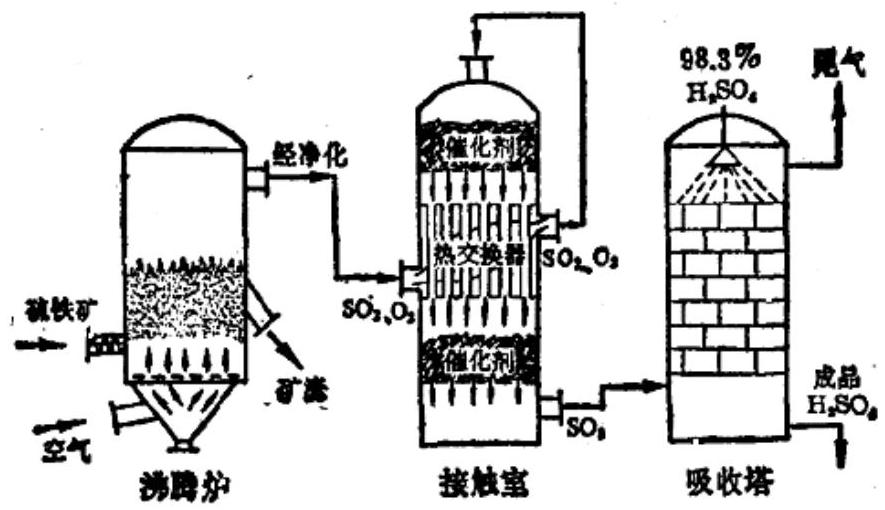
\includegraphics[max width=1.0\textwidth]{images/01912d0f-097c-7e75-8f32-4f326cd86c9f_66_413784.jpg}
\end{center}

图 3-2 接触法制硫酸的简单流程示意图

从沸腾炉里出来的气体叫做炉气, 其中含有二氧化硫、氧气、氮气、水蒸气以及一些杂质, 如砷、硒等的化合物和矿尘等。杂质和矿尘都会使催化剂作用减弱或失去作用,这种现象叫做催化剂中毒。水蒸气对设备和生产也有不良影响。因此, 在进行氧化反应以前, 必须使炉气通过除尘(除去矿尘)、 洗涤 (除去砷、硒等的化合物)、干燥(除去水蒸气) 等净化设备来除去这些有害物质。这样处理过的混和气体主要含有二氧化硫、氧气和氮气。

\section*{2. 二氧化硫氧化成三氧化硫}

把二氧化硫跟氧气的混和气体加热到一定温度(400- \({500}^{ \circ }\mathrm{C}\) ),再通过适当的催化剂(例如五氧化二钒等),二氧化硫就被氧气所氧化, 生成三氧化硫, 同时放出大量的热。它的热化学方程式是:

\[
2{\mathrm{{SO}}}_{2}\left( \text{ 气 }\right) + {\mathrm{O}}_{2}\left( \text{ 气 }\right) \frac{\text{ 催化剂 }}{\bigtriangleup }2{\mathrm{{SO}}}_{3}\left( \text{ 气 }\right) + {47}\text{ 千卡 }
\]

二氧化硫氧化成三氧化硫的反应是在接触室 (或叫转化器, 见图 3-2) 里进行的。在两层催化剂中间装有一个热交换器, 用来把反应时生成的热, 传递给进入接触室的需要预热的混和气体并冷却反应后生成的气体。象这样传递热量的过程就是化学工业上常用的热交换过程。

经过热交换器, 为二氧化硫的接触氧化和三氧化硫的吸收创造了有利条件。

\begin{center}
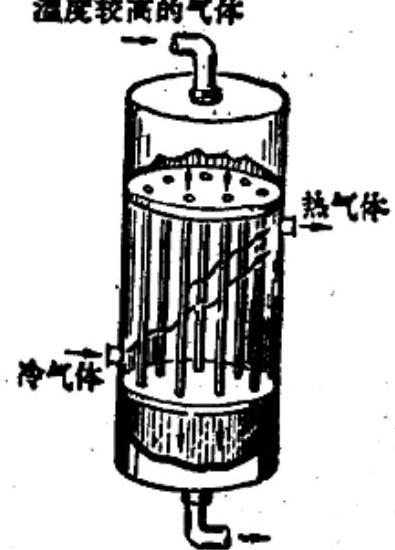
\includegraphics[max width=0.4\textwidth]{images/01912d0f-097c-7e75-8f32-4f326cd86c9f_67_562896.jpg}
\end{center}

温度较低的气体

热交换器是化学工业里广泛应用的热交换设备, 它有各种形式。多数热交换器的内部, 装有许多平行的管道或蛇管, 以扩大传热面, 提高换热效果。一种流体在管道里流动, 另一种流体在管道外流动。两种流体通过管壁进行热交换, 热的流体得到冷却, 冷的流体得到加热。

根据使用目的的不同,热交换器可以用作冷却器、加热器、冷凝器 图 3-3 热交换器示意图和汽化器等, 以便在反应过程里调节流体温度、利用余热等。

图 3-3 是常见的一种热交换器。

\section*{3. 三氧化硫的吸收和硫酸的生成}

从接触室出来的气体, 主要是三氧化硫和氮气以及剩余的未起反应的氧气和二氧化硫。

三氧化硫跟水化合生成硫酸, 同时放出大量的热。

\[
{\mathrm{{SO}}}_{3} + {\mathrm{H}}_{2}\mathrm{O} = {\mathrm{H}}_{2}{\mathrm{{SO}}}_{4}
\]

[讨论] 用最简便的解法,计算用接触法制造 50 吨98\% 的浓硫酸,在理论上需要多少吨含 \({\mathrm{{FeS}}}_{2}{70}\%\) 的硫铁矿。

硫酸虽然是三氧化硫黑水化合而制得的,但工业上不是直接用水或稀硫酸来吸收三氧化硫的。因为用水或稀硫酸作吸收剂时, 容易形成酸雾, 吸收速度慢, 不利于吸收三氧化硫。 为了尽可能把三氧化硫吸收干净, 并在吸收过程中不形成酸雾,工业上是用 \({98.3}\%\) 的硫酸来吸收三氧化硫的。

吸收过程是在吸收塔 (图 3-2) 里进行的。在吸收塔里, 三氧化硫从塔的下部通入, \({98.3}\%\) 的硫酸从塔顶喷下,成品硫酸从塔底放出。98.3\% 的硫酸吸收三氧化硫后浓度增大, 把这样制得的硫酸用水或稀硫酸稀释, 成为各种浓度的硫酸。

从吸收塔上部导出的没有起反应的氧气和少量的二氧化硫, 以及不起反应的氮气等气体, 工业上叫做尾气。这些尾气从塔的上部的出气管排出。

\section*{二、尾气中二氧化硫的回收和环境保护}

接触法制硫酸的尾气中, 还含有少量的二氧化硫等, 如果排入大气,就会造成环境污染。二氧化硫是大气污染的主要有害物质之一。排入大气的二氧化硫往往和飘尘结合在一起, 被吸入人体内部; 会引起呼吸道疾病。二氧化硫跟鼻、咽粘膜的水分结合, 生成酸性物质, 发生刺激作用。当大气里二氧化硫含量较多时, 人们就会咳嗽、打喷嚏、流涕、流泪和气管发炎。室内二氧化硫长期含量多, 就会发生严重后果。二氧化硫还可直接伤害农作物, 造成减产, 甚至使植株完全枯死, 颗粒无收。二氧化硫还跟空气中的水蒸气结合, 变成“酸雾”, 随雨雪降到地面,导致土壤酸化。这种“酸雾”的毒性比二氧化硫大得多, 而且可以吹到很远的地方, 对人体、生物、物品的危害更大。因此, 在尾气排放到大气中以前, 必须回收处理, 防止二氧化硫污染大气, 以保护环境, 并充分利用原料。

尾气中二氧化硫的回收,常常采用氨吸收法。这种方法是用氨水作为吸收剂除去尾气中的二氧化硫。反应的化学方程式是:

\[
{\mathrm{{SO}}}_{2} + 2{\mathrm{{NH}}}_{3} + {\mathrm{H}}_{2}\mathrm{O} = {\left( {\mathrm{{NH}}}_{4}\right) }_{2}{\mathrm{{SO}}}_{8}
\]

\[
\text{亚硫酸铵}
\]

\[
{\left( {\mathrm{{NH}}}_{4}\right) }_{2}{\mathrm{{SO}}}_{3} + {\mathrm{{SO}}}_{2} + {\mathrm{H}}_{2}\mathrm{O} = 2{\mathrm{{NH}}}_{4}{\mathrm{{HSO}}}_{3}
\]

\[
\text{亚硫酸氢铵}
\]

当吸收液中亚硫酸氢铵达到一定浓度后,再跟浓硫酸(浓度为 93,\%)反应,放出二氧化硫气体,同时得到硫酸铵溶液。反应的化学方程式是:

\[
2{\mathrm{{NH}}}_{4}{\mathrm{{HSO}}}_{3} + {\mathrm{H}}_{2}{\mathrm{{SO}}}_{4} = 2{\mathrm{{SO}}}_{2} \uparrow + 2{\mathrm{H}}_{2}\mathrm{O} + {\left( {\mathrm{{NH}}}_{4}\right) }_{2}{\mathrm{{SO}}}_{4}
\]

\[
{\left( {\mathrm{{NH}}}_{4}\right) }_{2}{\mathrm{{SO}}}_{3} + {\mathrm{H}}_{2}{\mathrm{{SO}}}_{4} = {\mathrm{{SO}}}_{2} \uparrow + {\mathrm{H}}_{2}\mathrm{O} + {\left( {\mathrm{{NH}}}_{4}\right) }_{2}{\mathrm{{SO}}}_{4}
\]

放出的二氧化硫气体浓度可达 \({95}\%\) 以上,可用于制液体二氧化硫。硫酸铵溶液经结晶、分离、干燥后制成固体 i酸铵肥料。这样, 尾气中的二氧化硫就可以回收利用。

硫酸厂排放的尾气里含有二氧化硫, 但是, 造成大气污染. 的二氧化硫, 大量的是由燃烧含硫的燃料如煤等产生的(其中包括家庭用煤在内)。此外, 一氧化碳、氮的氧化物、碳氢化合物以及粉尘等固体颗粒也会造成对大气的污染。

环境污染包括大气污染、水污染、土壤污染、食品污染、噪声等等。

环境污染的产生和发展, 跟人类的活动有着密切的联系。 人类在同自然界的斗争中, 通过劳动, 一方面, 不断地改造自然, 使人们的劳动和生活条件不断地得到改善; 另一方面, 由于不合理的管理制度,或受人们的认识能力以及科学技术水平的限制, 也带来对环境的污染和破坏。

工业 “三废” (即所谓废气、废水和废渣) 等对环境的污染, 许多是由于资源的综合利用水平低或没有综合利用等原因而造成的。因此, 我们必须采取积极措施, 努力消除和预防经济发展可能带来对环境的污染, 不断保护和改善环境, 为人民创建一个美好的劳动和生活环境。

\section*{习 题}

1. 接触法制硫酸的生产过程分为哪几个主要阶段?写出各阶段主要反应的化学方程式。

2. 计算 1 吨二氧化硫氧化成三氧化硫, 放出多少热量。

3. 回答下列问题:

(1)为什么用沸腾炉焙烧矿石制取二氧化硫时,要把矿石粉碎成细小的矿粒?

(2)为什么通入接触室的混和气体必须预先净化?

(3)为什么硫酸厂的尾气未经处理不准直接排入大气?

4. 燃烧 1 吨含硫 48\% 的硫铁矿,在理论上能生产多少

\section*{第四节 硫酸 硫酸盐}

\section*{一、硫酸}

\section*{1. 硫酸的性质}

硫酸在水溶液里很容易电离生成氢离子 \({}^{\left( 1\right) }\) 。

\[
{\mathrm{H}}_{2}{\mathrm{{SO}}}_{4} = 2{\mathrm{H}}^{ + } + {\mathrm{{SO}}}_{4}^{2 - }
\]

硫酸除了具有酸的通性以外, 还具有一些特性。

\({98.3}\%\) 的硫酸的沸点是 \({338}^{ \circ }\mathrm{C}\) 。硫酸是一种难挥发的强酸。

浓硫酸具有强烈的吸水性、脱水性和氧化性。我们在初中已经学习了浓硫酸的吸水性和脱水性, 现在进一步研究它的氧化性。

在常温下, 浓硫酸跟某些金属如铁、铝等接触, 能够使金属表面生成一薄层致密的氧化物保护膜 \({}^{\beta 2}\) ,阻止内部金属 继续跟硫酸起反应。因此, 浓硫酸可以用铁或铝的容器贮存。但是, 在受热的情况下, 浓硫酸不仅能够跟铁、铝等起反应, 而且能够跟绝大多数金属起反应。

[实验 3-6] 在试管里放入一块铜片, 注入少量浓硫酸, 给试管加热。观察试管里所起的变化。用润湿的蓝色石蕊试纸放在试管口检验所放出的气体。观察试纸颜色的变化。把试管里的溶液倒在盛着少量水的另一个试管里, 使溶液稀释, 观察溶液的颜色。

\customfootnote{

① 严格地说, 硫酸在水的作用下, 两个氢离子是分步电离的, 即先电离出第一个氢离子, 再电离出第二个氢离子。

第一步: \({\mathrm{H}}_{2}{\mathrm{{SO}}}_{4} = {\mathrm{H}}^{ + } + {\mathrm{{HSO}}}_{4} -\)

第二步: \({\mathrm{{HSO}}}_{4}^{ - } = {\mathrm{H}}^{ + } + {\mathrm{{SO}}}_{4}^{2 - }\)

② 这种现象叫做金属的钝化。

}

从上面的实验可以知道, 浓硫酸跟金属的反应不是置换反应, 不放出氢气。这个反应的生成物, 除该金属的硫酸盐外, 一般还有二氧化硫和水。

浓硫酸跟铜起反应的化学方程式如下:

\[
2{\mathrm{H}}_{2}{\mathrm{{SO}}}_{4}\text{ (浓) } + \mathrm{{Cu}}\overset{\bigtriangleup }{ \rightleftharpoons }{\mathrm{{CuSO}}}_{4} + 2{\mathrm{H}}_{2}\mathrm{O} + {\mathrm{{SO}}}_{2} \uparrow
\]

在这个反应里, 浓硫酸氧化了铜(铜从 0 价升高到 +2价), 它本身被还原成二氧化硫 (硫从 +6 价降低到 +4 价)。浓硫酸是氧化剂, 铜是还原剂。

当加热时, 浓硫酸还能够跟一些非金属起氧化- 还原反应。例如, 把浓硫酸跟木炭一起放在试管里, 并给试管加热, 木炭里的碳就被氧化成二氧化碳, 而硫酸被还原为二氧化硫。

\[
2{\mathrm{H}}_{2}{\mathrm{{SO}}}_{4}\text{ (浓) } + \mathrm{C}\overset{\Delta }{ = }{\mathrm{{CO}}}_{2} \uparrow + 2{\mathrm{H}}_{2}\mathrm{O} + 2{\mathrm{{SO}}}_{2} \uparrow
\]

在这个反应里, 浓硫酸是氧化剂, 碳是还原剂。

由此可见, 浓硫酸是强氧化剂, 它具有强氧化性。

\section*{2. 硫酸的用途}

硫酸是化学工业中最重要的产品之一。根据硫酸的各种不同的性质, 硫酸在工业上和实验室里具有十分广泛的用途。 在化学肥料工业上, 利用硫酸跟磷矿粉起反应可制得过磷酸钙等磷肥; 利用它跟氨或氨水的反应可制得氮肥硫酸铵。在金属加工和金属制品进行电镀以前, 可以利用硫酸跟金属氧化物起反应的性质来除去金属表面的氧化物。利用硫酸能跟金属或金属氧化物起反应的性质可以制出许多有实用价值的硫酸盐, 如硫酸铜、硫酸亚铁, 等等。因为硫酸是一种高沸点酸, 可以用它来制取各种挥发性酸, 如跟氟化钙起反应制得氟化氢, 溶于水生成氢氟酸。硫酸还用于精炼石油, 制造炸药、 农药、染料,等等。

在化学实验室里, 硫酸是一种常用的试剂。利用浓硫酸的吸水作用, 通常也把它用作干燥剂。

\section*{二、硫酸盐}

硫酸盐的种类很多, 有的在实际应用上很有价值。在初中化学里已经学过一些重要的硫酸盐, 如硫酸铜、硫酸铵等。 现在, 我们再来认识几种重要的硫酸盐。

\section*{1. 硫酸钙 \(\left( {\mathrm{{CaSO}}}_{4}\right)\)}

硫酸钙是白色固体。带两个分子结晶水的硫酸钙, 叫做石膏 \(\left( {{\mathrm{{CaSO}}}_{4} \cdot 2{\mathrm{H}}_{2}\mathrm{O}}\right)\) 。石膏在自然界以石膏矿大量存在。给石膏加热到 \({150} - {170}^{ \circ }\mathrm{C}\) 时,石膏就失去所含大部分结晶水而变成熟石膏 \(\left( {2{\mathrm{{CaSO}}}_{4} \cdot {\mathrm{H}}_{2}\mathrm{O}}\right)\) 。熟石膏跟水混和成糊状物后很快凝固, 重新变成石膏。人们利用这种性质, 通常把石膏用来制造各种模型。医疗上用它来作石膏绷带。水泥厂也要用石膏来调节水泥的凝结时间。

\section*{2: 硫酸锌 \(\left( {\mathrm{{ZnSO}}}_{4}\right)\)}

带七个分子结晶水的硫酸锌 \(\left( {{\mathrm{{ZnSO}}}_{4} \cdot 7{\mathrm{H}}_{2}\mathrm{O}}\right)\) ,是无色的晶体, 俗称皓矾。医疗上用作收敛剂, 可使有机体组织收缩, 减少腺体的分泌; 在铁路施工上用它的溶液来浸枕木, 是木材的防腐剂; 在印染工业上用它能使染料固着于纤维上, 是一种媒染剂。硫酸锌又可用于制造白色颜料(锌钡白等)。

\section*{3. 硫酸钡 \(\left( {\mathrm{{BaSO}}}_{4}\right)\)}

硫酸钡可作白色颜料。天然产的硫酸钡叫做重晶石。重晶石是制造其它钡盐的原料。硫酸钡不溶于水, 也不溶于酸。 利用这种性质以及不容易被 \(\mathbf{X}\) 射线透过的性质,医疗上常用硫酸钡作 \(\mathrm{X}\) 射线透视肠胃的内服药剂,俗称“钡餐”。

\section*{三、硫酸根离子的检验}

硫酸和硫酸盐溶于水时都会产生硫酸根离子。可以利用硫酸钡的不溶性来检验硫酸根离子的存在。

[实验 3-7] 在分别盛着硫酸、硫酸钠、碳酸钠溶液的试管里, 各滴入少量氯化钡溶液, 在三个试管里都有白色沉淀生成。等沉淀下沉, 倒去上面的溶液, 再各注入少量盐酸或稀硝酸, 振荡试管, 观察有什么现象?

在硫酸或硫酸钠的溶液里加入氯化钡溶液, 就生成白色的硫酸钡沉淀。

\[
{\mathrm{{BaCl}}}_{2} + {\mathrm{H}}_{2}{\mathrm{{SO}}}_{4} = {\mathrm{{BaSO}}}_{4} \downarrow + 2\mathrm{{HCl}}
\]

\[
{\mathrm{{BaCl}}}_{2} + {\mathrm{{Na}}}_{2}{\mathrm{{SO}}}_{4} = {\mathrm{{BaSO}}}_{4} \downarrow + 2\mathrm{{NaCl}}
\]

在碳酸钠的溶液里加入氯化钡溶液, 也生成白色沉淀, 这是碳酸钡沉淀。

\[
{\mathrm{{BaCl}}}_{2} + {\mathrm{{Na}}}_{2}{\mathrm{{CO}}}_{3} = {\mathrm{{BaCO}}}_{3} \downarrow + 2\mathrm{{NaCl}}
\]

从上面的实验还可以看到, 白色硫酸钡既不溶于水, 也不溶于盐酸或稀硝酸, 但白色碳酸钡能够溶于盐酸或稀硝酸。

\[
{\mathrm{{BaCO}}}_{3} + 2\mathrm{{HCl}} = {\mathrm{{BaCl}}}_{2} + {\mathrm{H}}_{2}\mathrm{O} + {\mathrm{{CO}}}_{2} \uparrow
\]

\[
{\mathrm{{BaCO}}}_{3} + 2{\mathrm{{HNO}}}_{3} = \mathrm{{Ba}}{\left( {\mathrm{{NO}}}_{3}\right) }_{2} + {\mathrm{H}}_{2}\mathrm{O} + {\mathrm{{CO}}}_{2} \uparrow
\]

许多不溶于水的钡盐(如磷酸钡)也跟碳酸钡一样, 能溶于盐酸或稀硝酸。

由此可见, 用可溶性钡盐溶液和盐酸(或稀硝酸) 可以检验硫酸根离子的存在。

\section*{习 题}

\section*{1. 下列现象反映了硫酸的哪些性质?}

(1)把浓硫酸滴入放在蒸发皿里的蔗糖 \(\left( {{\mathrm{C}}_{12}{\mathrm{H}}_{22}{\mathrm{O}}_{11}}\right)\) 上, 蔗糖就炭化变黑。

(2)硫酸跟氯化钠起反应,可能生成 \({\mathrm{{NaHSO}}}_{4}\) 和 \({\mathrm{{Na}}}_{2}{\mathrm{{SO}}}_{4}\) 两种盐。

(3)把浓硫酸霉置空气里,质量会增加。

(4)把锌粒放入稀硫酸里,会产生氢气。

(5)把铜片放入浓硫酸里并加热,会产生二氧化硫。

2. 到现在为止, 你已经知道, 在实验室里利用硫酸跟其它物质起反应, 可以制出哪几种气体来? 写出它们的化学方程式。

3. 为什么石膏可以用来制造各种模型, 以及医疗上用来作石膏绷带?

4. 怎样鉴别硫酸钡和碳酸钡7写出有关反应的化学方程式。

5. 用什么方法鉴别硫化钾和硫酸钾?

\section*{第五节 离子反应 离子方程式}

\section*{一、离子反应 离子方程式}

在初中化学里, 我们已经学过电解质溶于水后就电离成为离子, 所以, 电解质在溶液里所起的反应实质上就是离子之间的反应。这样的反应属于离子反应。

上节讲到的硫酸或硫酸钠溶液跟氯化钡溶液所起的反应, 就是电解质在溶液里的离子反应。现在我们分析一下硫酸钠溶液跟氯化钡溶液起反应的情况。

硫酸钠溶液跟氯化钡溶液起反应, 生成氯化钠和白色的硫酸钡沉淀。

\[
{\mathrm{{BaCl}}}_{2} + {\mathrm{{Na}}}_{2}{\mathrm{{SO}}}_{4} = 2\mathrm{{NaCl}} + {\mathrm{{BaSO}}}_{4} \downarrow
\]

如把易溶的、易电离的物质写成离子的形式, 把难溶的物质、难电离的物质或气体用分子式来表示, 可写成下式:

\[
{\mathrm{{Ba}}}^{2 + } + 2{\mathrm{{Cl}}}^{ - } + 2{\mathrm{{Na}}}^{ + } + {\mathrm{{SO}}}_{4}^{2 - } = 2{\mathrm{{Na}}}^{ + } + 2{\mathrm{{Cl}}}^{ - } + {\mathrm{{BaSO}}}_{4} \downarrow
\]

在溶液里开始时存在四种离子,由于 \({\mathrm{{Ba}}}^{2 + }\) 跟 \({\mathrm{{SO}}}_{4}^{2 - }\) 结合而成难溶于水的 \({\mathrm{{BaSO}}}_{4}\) 沉淀,溶液里的 \({\mathrm{{Ba}}}^{2 + }\) 和 \({\mathrm{{SO}}}_{4}^{2 - }\) 迅速减少, 反应向右进行。

从上式可以看出,反应前后 \({\mathrm{{Na}}}^{ + }\) 和 \({\mathrm{{Cl}}}^{ - }\) 没有变化,把它们从式子中删去, 可写成下式:

\[
{\mathrm{{Ba}}}^{2 + } + {\mathrm{{SO}}}_{4}^{2 - } = {\mathrm{{BaSO}}}_{4} \downarrow
\]

上式表明, 硫酸钠溶液跟氯化钡溶液起反应, 实际参加反应的离子是 \({\mathrm{{Ba}}}^{2 + }\) 和 \({\mathrm{{SO}}}_{4}^{2 - }\) 。这种用实际参加反应的离子的符号来表示离子反应的式子叫离子方程式。

综上所述, 我们知道任何可溶性钡盐跟硫酸或可溶性硫酸盐之间的反应, 都可以用上述这个离子方程式来表示。因为在所有这种情况下,都会发生同样的化学反应: \({\mathrm{{Ba}}}^{2 + }\) 跟 \({\mathrm{{SO}}}_{4}^{2 - }\) 结合生成 \({\mathrm{{BaSO}}}_{4}\) 沉淀的反应。

由此可见, 离子方程式跟一般化学方程式不同。离子方程式不仅表示一定物质间的某个反应, 而且表示了所有同一类型的离子反应。

怎样书写离子方程式呢? 我们以硝酸钡溶液跟硫酸钠溶液的反应为例, 说明书写离子方程式的步骤。

第一步, 写出反应的化学方程式:

\[
\mathrm{{Ba}}{\left( {\mathrm{{NO}}}_{3}\right) }_{2} + {\mathrm{{Na}}}_{2}{\mathrm{{SO}}}_{4} = {\mathrm{{BaSO}}}_{4} \downarrow + 2{\mathrm{{NaNO}}}_{3}
\]

第二步, 把易溶的、易电离的物质写成离子形式, 难溶的物质或难电离的物质(例如水)以及气体等仍以分子式表示。

\[
{\mathrm{{Ba}}}^{2 + } + 2{\mathrm{{NO}}}_{3}{}^{ - } + 2{\mathrm{{Na}}}^{ + } + {\mathrm{{SO}}}_{4}^{2 - } = {\mathrm{{BaSO}}}_{4} \downarrow + 2{\mathrm{{Na}}}^{ + } + 2{\mathrm{{NO}}}_{3}{}^{ - }
\]

第三步, 删去式子两边不参加反应的离子:

\[
{\mathrm{{Ba}}}^{2 + } + {\mathrm{{SO}}}_{4}^{2 - } = {\mathrm{{BaSO}}}_{4} \downarrow
\]

第四步, 检查式子两边各元素的原子个数和电荷数是否相等。

\section*{二、离子反应发生的条件}

我们学习的复分解反应, 实质上是两种电解质在溶液中相互交换离子的反应。这类离子反应发生的条件是:

1. 生成难溶的物质 例如, 硝酸银溶液跟氯化钠溶液起反应,就是 \({\mathrm{{Ag}}}^{ + }\) 跟 \({\mathrm{{Cl}}}^{ - }\) 结合而生成氯化银沉淀,溶液里的 \({\mathrm{{Ag}}}^{ + }\) 和 \({\mathrm{{Cl}}}^{ - }\) 迅速减少,反应向右进行。

\[
{\mathrm{{AgNO}}}_{3} + \mathrm{{NaCl}} = {\mathrm{{NaNO}}}_{3} + \mathrm{{AgCl}} \downarrow
\]

离子方程式是: \({\mathrm{{Ag}}}^{ + } + {\mathrm{{Cl}}}^{ - } = \mathrm{{AgCl}} \downarrow\)

2. 生成难电离的物质 (如水) 例如, 硫酸跟氢氧化钠溶液起反应,就是酸里的 \({\mathrm{H}}^{ + }\) 跟碱里的 \({\mathrm{{OH}}}^{ - }\) 结合而生成难电离的水,溶液里的 \({\mathrm{H}}^{ + }\) 和 \({\mathrm{{OH}}}^{ - }\) 迅速减少,反应向右进行。

\[
{\mathrm{H}}_{2}{\mathrm{{SO}}}_{4} + 2\mathrm{{NaOH}} = {\mathrm{{Na}}}_{2}{\mathrm{{SO}}}_{4} + 2{\mathrm{H}}_{2}\mathrm{O}
\]

离子方程式是: \({\mathrm{H}}^{ + } + {\mathrm{{OH}}}^{ - } = {\mathrm{H}}_{2}\mathrm{O}\)

这个离子方程式说明了酸跟碱起中和反应的实质,是 \({\mathrm{H}}^{ + }\) 跟 \({\mathrm{{OH}}}^{ - }\) 结合成 \({\mathrm{H}}_{2}\mathrm{O}\) 的反应。

3. 生成挥发性的物质 例如, 碳酸钠溶液跟盐酸起反应时, \({\mathrm{{CO}}}_{3}{}^{2 - }\) 跟 \({\mathrm{H}}^{ + }\) 结合而生成 \({\mathrm{H}}_{2}{\mathrm{{CO}}}_{3},{\mathrm{H}}_{2}{\mathrm{{CO}}}_{3}\) 不稳定,分解成水和二氧化碳气体,溶液里的 \({\mathrm{{CO}}}_{3}^{2 - }\) 和 \({\mathrm{H}}^{ + }\) 迅速减少,反应向右进行。

\[
{\mathrm{{Na}}}_{2}{\mathrm{{CO}}}_{3} + 2\mathrm{{HCl}} = 2\mathrm{{NaCl}} + {\mathrm{H}}_{2}\mathrm{O} + {\mathrm{{CO}}}_{2} \uparrow
\]

离子方程式是: \({\mathrm{{CO}}}_{3}{}^{2 - } + 2{\mathrm{H}}^{ + } = {\mathrm{H}}_{2}\mathrm{O} + {\mathrm{{CO}}}_{2} \uparrow\)

凡具备上述条件之一, 这类离子反应就能发生。

如果把氯化钠溶液跟硝酸钙溶液混和在一起, 它们之间是否发生离子反应呢? 让我们来分析一下氯化钠溶液跟硝酸钙溶液混和后溶液里的情况。

\[
2\mathrm{{NaCl}} + \mathrm{{Ca}}{\left( {\mathrm{{NO}}}_{3}\right) }_{2} = 2{\mathrm{{NaNO}}}_{3} + {\mathrm{{CaCl}}}_{2}
\]

\(2{\mathrm{{Na}}}^{ + } + 2{\mathrm{{Cl}}}^{ - } + {\mathrm{{Ca}}}^{2 + } + 2{\mathrm{{NO}}}_{3}^{ - } = 2{\mathrm{{Na}}}^{ + } + 2{\mathrm{{NO}}}_{3}{}^{ - } + {\mathrm{{Ca}}}^{2 + } + 2{\mathrm{{Cl}}}^{ - }\)

从上式可以看出, 式子里的等号前后都是同样的四种离子,这四种离子混和后没有起反应而生成沉淀或气体或难电离的物质 (如水), 也就是说, 没有发生离子反应。

离子反应除上面讲的以离子互换形式进行的复分解反应外, 还有其它类型的反应, 例如, 有离子参加的置换反应, 等等。

例 1: \(\mathrm{{Zn}} + 2\mathrm{{HCl}} = {\mathrm{{ZnCl}}}_{2} + {\mathrm{H}}_{2} \uparrow\)

离子方程式是: \(\mathrm{{Zn}} + 2{\mathrm{H}}^{ + } = {\mathrm{{Zn}}}^{2 + } + {\mathrm{H}}_{2} \uparrow\)

例 2: \({\mathrm{{Cl}}}_{2} + 2\mathrm{{KI}} = 2\mathrm{{KCl}} + {\mathrm{I}}_{2}\)

离子方程式是: \({\mathrm{{Cl}}}_{2} + 2{\mathrm{I}}^{ - } = 2{\mathrm{{Cl}}}^{ - } + {\mathrm{I}}_{2}\)

\section*{习 题}

1. 下面有六组物质。对能起反应的, 写出化学方程式 (离子反应需要写出离子方程式,氧化-还原反应需要指出电子的转移, 并指出氧化剂和还原剂); 对不能起反应的, 说明不起反应的理由。

(1)硫酸钠溶液跟氯化钡溶液;

(2)盐酸跟氢氧化钠溶液;

\begin{center}
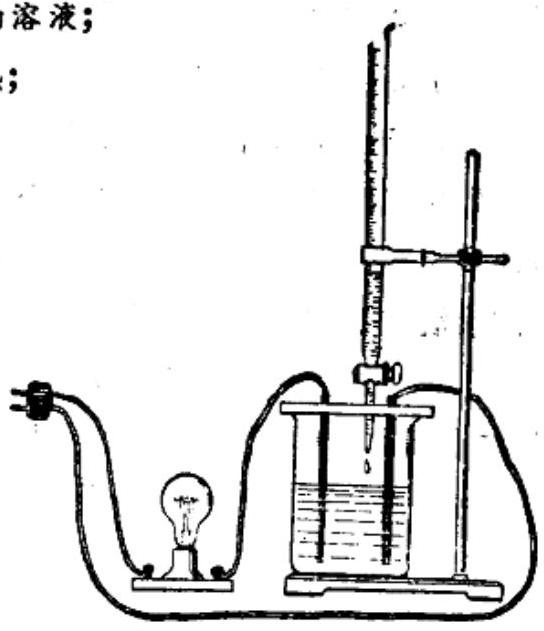
\includegraphics[max width=0.6\textwidth]{images/01912d0f-097c-7e75-8f32-4f326cd86c9f_79_583876.jpg}
\end{center}

(3)浓硫酸跟铜加热;

(4) 盐酸跟碳酸钙;

(5) 硝酸钠溶液跟

氣酸鉀溶液;

(6)硫化亚铁跟稀盐酸。

2. 利用图 3-4 的装置来做下面的实验: 先在玻璃容器里盛半杯氢氧化钡溶液, 然后由滴定管

向容器里浦入硫酸溶液。 图 3-4 液体导电性的实验装置示意图随着硫酸的滴入, 电灯就渐渐变暗, 最后电灯完全熄灭。为什么? 这时如果继续滴入硫酸, 电灯又会逐渐亮起来, 为什么?在滴入硫酸的同时,看到了在溶液里有什么现象?如果用盐酸代替硫酸, 能观察到同样现象吗? 为什么?

3. 写出能实现下列变化的相应的化学方程式。

(1) \({\mathrm{{Cu}}}^{2 + } + 2{\mathrm{{OH}}}^{ - } = \mathrm{{Cu}}{\left( \mathrm{{OH}}\right) }_{2} \downarrow\)

(2) \({\mathrm{H}}^{ + } + {\mathrm{{OH}}}^{ - } = {\mathrm{H}}_{2}\mathrm{O}\)

(3) \(2{\mathrm{H}}^{ + } + {\mathrm{{CaCO}}}_{3} = {\mathrm{{Ca}}}^{2 + } + {\mathrm{H}}_{2}\mathrm{O} + {\mathrm{{CO}}}_{2} \uparrow\)

(4) \(2{\mathrm{H}}^{ + } + {\mathrm{{CO}}}_{3}{}^{2 - } = {\mathrm{H}}_{2}\mathrm{O} + {\mathrm{{CO}}}_{2} \uparrow\)

(5) \({\mathrm{{Cu}}}^{2 + } + \mathrm{{Fe}} = {\mathrm{{Fe}}}^{2 + } + \mathrm{{Cu}} \downarrow\)

4. 两个试管里分别盛有氢氧化钠溶液和氢氧化钡溶液, 怎样鉴别它们?写出反应的化学方程式和离子方程式。

5. 现有稀硫酸、稀盐酸、硫酸钠、碳酸钠、氯化钠等五种无色溶液, 试用化学方法把它们检验出来, 并写出反应的化学方程式和离子方程式。

\section*{第六节 氧 族 元 素}

氧和硫是氧族元素里具有代表性的元素。

氧族元素 \({}^{\left( 1\right) }\) 里的 硒、碲也跟硫一样,都能跟氢生成气态的化合物。它们的氢化物的水溶液都显酸性, 在氢化物里, 它们都显 -2 价。

除了氧以外, 硫、硒、碲都有二氧化物和三氧化物, 在三氧化物里显示出它们的最高化合价: +6。这些氧化物对应的水化物都是酸。

\customfootnote{

① 氧族元素里的钋在地壳里是一种非常稀少的元素, 在本节中不讨论它的性质。

}

二氧化物 对应的水化物 三氧化物 对应的水化物

\({\text{SO}}_{2}\;{\text{H}}_{2}{\text{SO}}_{3}\;{\text{SO}}_{3}\;{\text{H}}_{2}{\text{SO}}_{4}\)

\({\text{SeO}}_{2}\;{\text{H}}_{2}{\text{SeO}}_{3}\;{\text{SeO}}_{3}\;{\text{H}}_{2}{\text{SeO}}_{4}\)

\({\text{TeO}}_{2}\;{\text{H}}_{2}{\text{TeO}}_{3}\;{\text{TeO}}_{3}\;{\text{H}}_{2}{\text{TeO}}_{4}\) ①

氧族元素跟大多数金属都能直接化合。

氧族元素性质的相似是由于它们的原子的电子层结构很相似, 这族元素的原子的最外电子层都各有 6 个电子。在化学反应里, 氧族元素的原子都容易从其它原子获得两个电子, 从而生成 -2 价的化合物; 它们的原子最外电子层的 6 个或 4 个电子一般也可以发生偏移, 生成 +6 价或 +4 价的化合物。

除了上述相似的性质外, 这四种元素的单质在性质方面还有一定的差别。

从表 3-1 可以看出, 氧、硫、硒、碲的单质的物理性质随核电荷数的增加而起着变化。它们的熔点、沸点随着核电荷数的增加而逐渐升高, 它们的密度随着核电荷数的增加而逐渐加大。此外, 硫不能导电, 硒是半导体, 而碲却能够导电。

氧、硫、硒、碲的单质的化学性质也随着核电荷数的增加而起变化。这四种单质跟氢气化合的时候, 氧气跟氢气的反应最容易, 也最剧烈, 生成的化合物也最稳定, 硫或硒跟氢气只有在较高的温度下才能够化合,而碲通常不能够跟氢气直接化合, 生成的化合物也最不稳定。这类元素(除氧外)的含

① 严格地说,碲酸通常以 \({\mathrm{H}}_{6}{\mathrm{{TeO}}}_{6}\) 和 \({\left( {\mathrm{H}}_{2}{\mathrm{{TeO}}}_{4}\right) }_{n}\) 两种形式存在. 氧酸的酸性一般也是随核电荷数的增加而逐渐减弱。

望科卵峯竺纲鏄 I-E 笨

\begin{center}
\adjustbox{max width=\textwidth}{
\begin{tabular}{|c|c|c|c|c|c|}
\hline
\multirow{2}{*}{等于} & 水化物 氧化物的 & 1 & \phantom{X} & HK \text{\textbackslash} \$’000HK \text{\textbackslash} \$’000 & HK \text{\textbackslash} \$’000HK \text{\textbackslash} \$’000 \\
\cline{2-6}
& 分子式 & 1 & \phantom{X} & So & TransitiveTransport \\
\hline
\multirow{3}{*}{參孔脣} & 稳定性 & \multicolumn{4}{|c|}{减小} \\
\cline{2-6}
& 化合条件 & 点燃或放心 & 加热 & 加热 & 不直接化合 \\
\cline{2-6}
& 分子式 & HK \text{\textbackslash} \$’000 & HK \text{\textbackslash} \$’000 & HK \text{\textbackslash} \$’000 & HHS \\
\hline
\multirow{5}{*}{质 单} & 密(s米面/ 3f) & 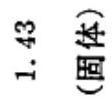
\includegraphics[max width=0.2\textwidth]{images/01912d0f-097c-7e75-8f32-4f326cd86c9f_82_525814.jpg} & 2,071 & 4,811 & 6,255 \\
\cline{2-6}
& 沸S & 1-34 & 4,646 & 684,4 & 133,393 \\
\cline{2-6}
& 点CO & 一2,848 & 112,823 & 2023 & 455 \\
\cline{2-6}
& 状态 & 气体 & 固体 & 固体 & 周体 \\
\cline{2-6}
& 颜色 & 无色 & 黄色 & 灰色 & 银白色 \\
\hline
\multicolumn{2}{|c|}{併將習士中} & . ) ) & ) 】 )2) & 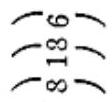
\includegraphics[max width=0.2\textwidth]{images/01912d0f-097c-7e75-8f32-4f326cd86c9f_82_525815.jpg} & 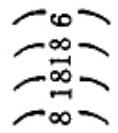
\includegraphics[max width=0.2\textwidth]{images/01912d0f-097c-7e75-8f32-4f326cd86c9f_82_525816.jpg} \\
\hline
\multicolumn{2}{|c|}{核电荷数} & \(\infty\) & 16 & 34 & 52 \\
\hline
\multicolumn{2}{|c|}{元素符号} & O & S & S & 几 \\
\hline
\multicolumn{2}{|c|}{元素名称} & 氧 & 硫 & 硒 & 储 \\
\hline
\end{tabular}
}
\end{center}

氧、硫、硒、碲等元素的性质的差异和递变跟它们的原子结构有关。随着核电荷数的增加, 这些元素的原子的电子层数增多, 原子或离子半径都增大 (图 3-5)。

\begin{center}
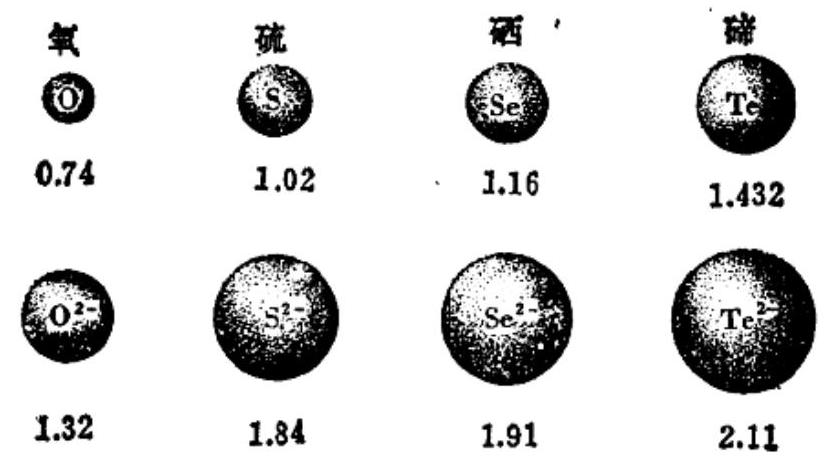
\includegraphics[max width=0.9\textwidth]{images/01912d0f-097c-7e75-8f32-4f326cd86c9f_83_843063.jpg}
\end{center}

图 3-5 氧族元素的原子和离子大小示意图 (数据单位是 \({10}^{-{10}}\) 米)

由于原子半径的逐渐增大, 因此, 核对外层电子的引力逐渐减弱, 使原子获得电子的能力依次减弱, 失去电子的倾向依次增强, 也就是说, 随着核电荷数的增加, 氧、硫、硒、碲等元素的金属性逐渐增强, 非金属性逐渐减弱。

\section*{习 题}

1. 氧、硫、硒、碲四种元素的性质有哪些相似点和不同点?

2. 氧族元素和卤族元素的性质有哪些相似点和不同点?

\section*{内容提要}

\section*{一、氧族元素}

氧、硫、硒、碲等氧族元素的原子结构很相似, 它们的最外电子层都各有 6 个电子, 在化学反应里容易得到电子, 显非金属性。随着核电荷数和电子层数的增加而原子半径增大, 氧、 硫、硒、碲等元素的原子获得电子的能力依次减弱, 它们的金属性逐渐增强, 而非金属性逐渐减弱。

\section*{二、硫的化学性质}

1. 硫能跟大多数金属反应, 生成金属硫化物。

2. 硫能跟氢气反应, 生成硫化氢。

硫化氢是一种还原剂, 它的水溶液氢硫酸是一种弱酸。

3. 硫能跟氧气起反应, 生成二氧化硫等。

三、硫的重要氧化物 \({2}^{\frac{2 - 1}{2}}\) 被计算、它关系 \(\mathcal{C}\) 成

1. 二氧化硫 二氧化硫易溶于水; 它跟米反应生成亚硫酸。亚硫酸不稳定, 容易分解成二氧化硫和水。这是一种可逆反应:

\[
{\mathrm{{SO}}}_{2} + {\mathrm{H}}_{2}\mathrm{O} = - {\mathrm{H}}_{2}{\mathrm{{SO}}}_{3}
\]

可逆反应是在同一条件下, 既能向正反应方向进行, 同时又能向逆反应方向进行的反应。

2. 三氧化硫 二氧化硫经催化氧化生成三氧化硫。三氧化硫跟水剧烈化合而生成硫酸。

\section*{四、硫酸}

1. 工业上用接触法制硫酸的主要化学反应

(1) \(4{\mathrm{{FeS}}}_{2} + {11}{\mathrm{O}}_{2}\xrightarrow[]{\text{ 高温 }}2{\mathrm{{Fe}}}_{2}{\mathrm{O}}_{3} + 8{\mathrm{{SO}}}_{2}\)

(2) \(2{\mathrm{{SO}}}_{2} + {\mathrm{O}}_{2}\frac{\text{ 催化剂 }}{\Delta }2{\mathrm{{SO}}}_{3}\)

(3) \({\mathrm{{SO}}}_{3} + {\mathrm{H}}_{2}\mathrm{O} = {\mathrm{H}}_{2}{\mathrm{{SO}}}_{4}\)

2. 防止污染, 保护环境

有些工业产生的废气、废水、废渣, 如硫酸厂排出的含二氧化硫的尾气, 污染环境, 必须回收处理, 加以综合利用, 防止污染大气、水源、土壤等, 为人民创建一个美好的劳动和生活环境。

3. 浓硫酸的特性: 吸水性、脱水性和氧化性。

4. 硫酸根离子的检验

用可溶性钡盐溶液和盐酸(或稀硝酸)来检验SO。 的存在。

五、离子反应和离子方程式

。。中学化学里讲的离子反应主要是指以离子互换形式进行的复分解反应。此外, 有离子参加的置换反应等也是离子反应。

属于复分解反应的这类离子反应发生的条件是, 生成难溶的或难电离的或挥发性的物质。

用实际参加反应的离子的符号来表示离子反应的式子叫做离子方程式。离子方程式不仅表示一定物质间的某个反应, 而且表示了所有同一类型的离子反应。

书写离子方程式时, 要写出实际参加反应的离子符号, 把难溶、难电离和挥发性的物质用分子式表示。

\section*{复习 题}

1. 写出实验室制取下列各种气体的化学方程式(离子反应还要写出离子方程式), 并说明收集这些气体的方法。

(1) 氧气,(2) 氯气,(3) 氯化氢,(4) 硫化氢,(5) 二氧化硫。

2. 浓硫酸和稀硫酸的性质有哪些不同的地方?

3. 回答下列问题:

(1)启普发生器常用于制取硫化氢气体,为什么不用于制取二氧化硫气体?

(2)用二氧化硫漂白过的草帽, 日久为什么会发黄?

(3)在接触法制硫酸的工厂中, 为什么不用水而用 \({98.3}\%\) 的硫酸来吸收三氧化硫?

4. \({\mathrm{H}}_{2}\mathrm{\;S}\text{、}\mathrm{\;S}\text{、}{\mathrm{H}}_{2}{\mathrm{{SO}}}_{4}\) 等三种物质中,哪种可作氧化剂,哪种可作还原剂, 哪种既可作氧化剂又可作还原剂? 举出具体反应来说明。

5. 写出铜跟浓硫酸、铁罩稀硫酸反应的化学方程式或离子方程式, 并指出这两个六 \(\lambda\) 中哪种物质被还原,哪种物质被氧化。

6. 含 \({\mathrm{{FeS}}}_{2}\;{72}\%\) 的硫铁矿在煅烧的时候,有 \({1.5}\%\) 的硫受到损失而混入炉渣,由这种硫铁矿 \(1\) 吨可以制等 \({98}\%\) 硫酸多少吨?

7. 用硫化亚铁跟稀盐酸起反应,把产生的气体导出点燃, 在火焰的附近用湿润的蓝色石蕊试纸试验, 试纸变成浅红色。用一个洁净的蒸发皿底靠近火焰,蒸发皿底附上了一层黄色粉末。说明发生以上现象的原因,并写出有关反应的化学方程式。

8. 在下列反应 \(\Omega\) ,二氧化硫是氧化剂还是还原剂,为什么?

(1) \(2{\mathrm{H}}_{2}\mathrm{\;S} + {\mathrm{{SO}}}_{2} = 3\mathrm{\;S} + 2{\mathrm{H}}_{2}\mathrm{O}\)

(2) \({\mathrm{{Br}}}_{2} + {\mathrm{{SO}}}_{2} + 2{\mathrm{H}}_{2}\mathrm{O} = {\mathrm{H}}_{2}{\mathrm{{SO}}}_{4} + 2\mathrm{{HBr}}\)

9. 写出下列物质变化的化学方程式(其中的离子反应还要写出相应的离子方程式):

\[
{\mathrm{{FeS}}}_{2} \rightarrow {\mathrm{{SO}}}_{2} \rightarrow {\mathrm{{SO}}}_{3} \rightarrow {\mathrm{H}}_{2}{\mathrm{{SO}}}_{4} \rightarrow {\mathrm{{CuSO}}}_{4} \rightarrow \mathrm{{Cu}}
\]

\section*{第四章 碱 金 属}

我们已经学习了卤族和氧族元素的知识, 对非金属元素有了一些认识。在这一章里, 我们将要学习一族叫做碱金属的金属元素。我们已经知道锂和钠的原子结构在最外电子层都只有 1 个电子。具有相似结构的还有钾等四种元素。碱金属包括锂、钠、钾、铷、铯、钫六种元素, 因为它们的氧化物的水化物是可溶于水的碱,所以统称为碱金属。本章主要介绍钠及其化合物的知识。

\section*{第一节 钠}

\section*{一、钠的物理性质}

[实验 4-1] 取一块金属钠, 用刀切去一端的外皮, 观察钠的颜色。

金属钠很软, 可以用刀切割。切开外皮后, 可以看到钠的 “真面目”呈银白色, 具有美丽的光泽。

钠是热和电的良导体, 密度 0.97 克/厘米 , 比水还轻, 能浮在水面上,熔点 \({97.81}^{ \circ }\mathrm{C}\) ,沸点 \({882.9}^{ \circ }\mathrm{C}\) 。

\section*{二、钠的化学性质}

钠的化学性质非常活泼。

\section*{1. 钠跟氧气的反应}

[实验 4-2] 用刀切开一小块钠, 观察在光亮的断面上所发生的变化。把小块钠放在燃烧匙里加热, 观察发生的变化。

钠很容易氧化, 在常温下就能够跟空气里的氧气化合而生成氧化物。切开的光亮的金属钠断面很快地发暗, 主要是因为生成了一薄层氧化物的缘故。钠受热以后能够在空气里着火燃烧, 在纯净的氧气里燃烧得更为剧烈, 燃烧时发出黄色的火焰。在钠跟氧气化合的过程中, 可以生成氧化钠, 氧化钠不稳定, 继续氧化, 生成过氧化钠。过氧化钠比较稳定, 所以钠在空气里燃烧, 生成的是过氧化钠。

\[
\begin{array}{r} 2\mathrm{{Na}} + {\mathrm{O}}_{2} = {\mathrm{{Na}}}_{2}{\mathrm{O}}_{2} \\ \text{ 过氧化钠 } \end{array}
\]

\section*{2. 钠跟硫等非金属的反应}

钠除了能跟氯气直接化合外,还能跟很多其它非金属直接化合, 如跟硫化合时甚至发生爆炸, 生成硫化钠。

\[
2\mathrm{{Na}} + \mathrm{S} = {\mathrm{{Na}}}_{2}\mathrm{\;S}
\]

\[
\text{硫化钠}
\]

\begin{center}
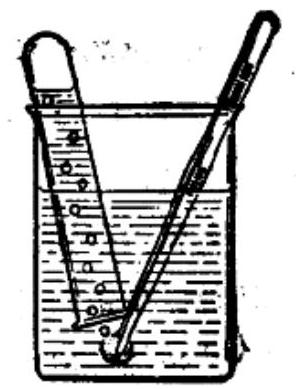
\includegraphics[max width=0.3\textwidth]{images/01912d0f-097c-7e75-8f32-4f326cd86c9f_89_628363.jpg}
\end{center}

\section*{3. 钠跟水的反应}

钠跟水能起剧烈的反应。

[实验 4-3] . 向一个盛有水 的烧杯里,滴入几滴酚酞溶液。然后把一小块钠(约等于 \(1/2\) 豌豆那么大小) 投

入烧杯里。注意观察钠跟水起反应的 图 4-1 钠跟水起反应情形和溶液颜色的变化。再用铝箔包好一小块钠, 并在铝箔上刺些小孔, 用镊子夹住, 放在试管口下面, 用排水法收集气体 (图 4-1)。小心地取出试管, 移近火焰, 检验试管里是不是收集了氢气。

投入烧杯里的钠比水轻, 浮在水面上。钠跟水起反应放出的热, 立刻使钠熔成一个闪亮的小球。小球向各个方向迅速游动, 并逐渐缩小, 最后完全消失。钠跟水起反应后, 使滴有酚酞溶液的水由无色变为红色。这个现象说明有别的物质生成,这种生成物就是氢氧化钠。试管里收集到的气体是氢气。

\[
2\mathrm{{Na}} + 2{\mathrm{H}}_{2}\mathrm{O} = 2\mathrm{{NaOH}} + {\mathrm{H}}_{2} \uparrow
\]

由于钠很容易跟空气里的氧气或水起反应, 所以通常保存在煤油里, 跟空气和水隔绝。

\section*{三、钠的存在}

钠的性质很活泼, 所以它在自然界里不能以游离态存在, 只能以化合态存在。钠的化合物在自然界里分布很广, 主要以氯化钠的形式存在, 也以硫酸钠、碳酸钠和硝酸钠等形式存在。

\section*{四、钠的制备和用途}

工业上, 可以把直流电通入熔融的氯化钠来制取钠。

钠可以用来制取过氧化钠等化合物。钠和钾的合金(含 \({50} - {80}\%\) 钾) 在室温下呈液态,是原子反应堆的导热剂。钠是一种很强的还原剂, 可以把钛、锆、铌、钽等金属从它们的熔融卤化物里还原出来。钠也应用在电光源上。高压钠灯发出的黄光射程远, 透雾能力强, 对道路平面的照度比高压水银灯高几倍。

\section*{习 题}

1. 金属的应该怎样保存?为什么?

2. 使 0.2 摩尔钠跟水起反应, 能生成多少升的氢气 (标准状况为

3. 钠着火时, 应选用下列哪种物质和器材灭火? 为什么?

(1) 水,(2) 泡沫灭火器,(3) 干粉灭火器。

\section*{第二节 钠的化合物}

\section*{一、钠的氧化物}

钠的氧化物有氧化钠和过氧化钠等。氧化钠是白色的固体, 跟水起剧烈的反应, 生成氢氧化钠。

\[
{\mathrm{{Na}}}_{2}\mathrm{O} + {\mathrm{H}}_{2}\mathrm{O} = 2\mathrm{{NaOH}}
\]

过氧化钠是淡黄色的固体, 也能跟水起反应, 生成氢氧化钠和氧气。

[实验 4-4] 把水滴入盛有过氧化钠固体的试管, 用带火星的木条放在管口, 检验有没有氧气放出。

\[
2{\mathrm{{Na}}}_{2}{\mathrm{O}}_{2} + 2{\mathrm{H}}_{2}\mathrm{O} = 4\mathrm{{NaOH}} + {\mathrm{O}}_{2} \uparrow
\]

过氧化钠是强氧化剂, 可以用来漂白织物、麦秆、羽毛等等。

过氧化钠跟二氧化碳起反应, 生成碳酸钠和氧气。

\[
2{\mathrm{{Na}}}_{2}{\mathrm{O}}_{3} + 2{\mathrm{{CO}}}_{3} = 2{\mathrm{{Na}}}_{2}{\mathrm{{CO}}}_{3} + {\mathrm{O}}_{2} \uparrow
\]

因此, 它用在呼吸面具上和潜水艇里作为氧气的来源。

\section*{二、钠的其它重要化合物}

我们在初中学过一种重要的钠的化合物一一氢氧化钠。 下面简单介绍几种重要的钠盐。

\section*{1. 硫酸钠}

硫酸钠晶体俗名芒硝 \(\left( {{\mathrm{{Na}}}_{2}{\mathrm{{SO}}}_{4} \cdot {10}{\mathrm{H}}_{2}\mathrm{O}}\right)\) 。硫酸钠是制玻璃和造纸 (制浆) 的重要原料, 也用在染色、纺织、制水玻璃等工业上,在医药上用作缓泻剂。自然界里的硫酸钠主要分布在盐湖和海水里。我国盛产芒硝。

\section*{2. 碳酸钠和碳酸氢钠}

碳酸钠 \(\left( {{\mathrm{{Na}}}_{2}{\mathrm{{CO}}}_{3}}\right)\) 俗名纯碱或苏打,是白色粉末。碳酸钠通常含结晶水 \(\left( {{\mathrm{{Na}}}_{2}{\mathrm{{CO}}}_{3} \cdot {10}{\mathrm{H}}_{2}\mathrm{O}}\right)\) 。在空气里碳酸钠晶体很容易失去结晶水, 表面失去光泽而逐渐发暗, 并渐渐碎裂成粉末。失水以后的碳酸钠叫做无水碳酸钠。碳酸氢钠(NaHCO \({}_{3}\) ) 俗名小苏打, 是一种细小的白色晶体。碳酸钠较碳酸氢钠容易溶解于水。

碳酸钠和碳酸氢钠遇到盐酸都能放出二氧化碳。

\[
{\mathrm{{Na}}}_{2}{\mathrm{{CO}}}_{3} + 2\mathrm{{HCl}} = 2\mathrm{{NaCl}} + {\mathrm{H}}_{2}\mathrm{O} + {\mathrm{{CO}}}_{2} \uparrow
\]

\[
{\mathrm{{NaHCO}}}_{3} + \mathrm{{HCl}} = \mathrm{{NaCl}} + {\mathrm{H}}_{2}\mathrm{O} + {\mathrm{{CO}}}_{2} \uparrow
\]

[实验 4-5] 把少量盐酸分别加入盛着碳酸钠和碳酸氢钠的两个试管里。比较它们放出二氧化碳的快慢程度。

碳酸氢钠遇到盐酸放出二氧化碳的作用, 要比碳酸钠剧烈得多。

碳酸钠很稳定, 受热很难分解, 碳酸氢钠却不很稳定, 受热容易分解。

[实验 4-6] 用图 4-2 的装置, 把碳酸钠放入试管里, 约占试管容积的 \(1/6\) ,并往烧杯里倒入石灰水。加热, 观察澄清的石灰水是否起变化。把试管拿掉, 换上一个放入同样容积. 碳酸氢钠的试管。再加热, 观察澄清的石灰水所起的变化。

\begin{center}
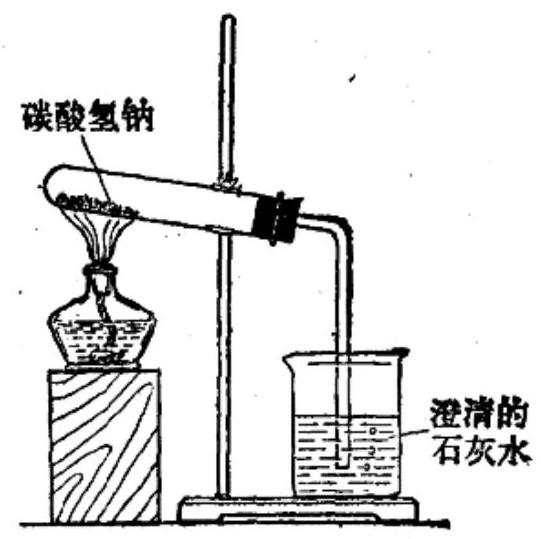
\includegraphics[max width=0.6\textwidth]{images/01912d0f-097c-7e75-8f32-4f326cd86c9f_93_618569.jpg}
\end{center}

图 4-2 鉴别碳酸钠和碳酸氢钠

碳酸钠受热没有变化, 而碳酸氢钠受热分解, 放出二氧化碳。

\[
2{\mathrm{{NaHCO}}}_{3}\overset{\bigtriangleup }{ = }{\mathrm{{Na}}}_{2}{\mathrm{{CO}}}_{3} + {\mathrm{H}}_{2}\mathrm{O} + {\mathrm{{CO}}}_{2} \uparrow
\]

这个反应可以用来鉴别碳酸钠和碳酸氢钠。

碳酸钠是化学工业的重要产品之一, 有很多用途。它广泛地用在玻璃、制皂、造纸、纺织等工业上, 也可以用来制造其它钠的化合物。日常生活里也常用它作洗涤剂。磷酸氢钠是焙制糕点所用的发酵粉的主要成分之一。在医疗上, 它是治疗胃酸过多的一种药剂。

碳酸钠有天然产出的。碱性土壤里和某些盐湖里常含有碳酸钠。我国内蒙古自治区一带的盐湖就出产大量的天然碱。

\section*{习 题}

1. 在呼吸面具里有时用到过氧化钠, 这利用了它的什么

性质?

2. 怎样断定某种碳酸钠粉末里是否含有碳酸氢钠?怎样把混在碳酸钠里的碳酸氢钠除去?

3. 写出下列各物质间转化的化学方程式 (其中离子反应还要写出相应的离子方程式)。

\[
\mathrm{{Na}} \rightarrow \mathrm{{NaOH}} \rightarrow \mathrm{{NaCl}} \rightarrow {\mathrm{{Na}}}_{2}{\mathrm{{SO}}}_{4}
\]

4. 空气里通常含有 \({0.05}\% {\mathrm{{CO}}}_{2}\) (质量百分比),计算 10 克的过氧化钠能够吸收多少升空气(标准状况)里的二氧化碳。

5. 加热 410 克小苏打到再没有气体放出时, 剩余的物质是什么?它的质量是多少克?

6. 把碳酸钠和碳酸氢钠的混和物 146 克加热到质量不再继续减少为止。剩下的残渣的质量是 137 克。计算这混和物里含有百分之几的碳酸钠?

\section*{第三节 碱金属元素}

\section*{一、碱金属元素的原子结构和碱金属的物理性质}

碱金属元素在自然界里都以化合态存在,它们的单质由人工制得。碱金属除铯略带金色光泽外, 都呈银白色, 碱金属都比较柔软, 有展性, 它们的密度较小, 熔点较低, 铯在气温稍高的时候, 就呈液态。它们的导热、导电的性能都很强。碱金属, 特别是锂、钠、钾, 是金属中比较轻的。表 4-1 列出各元素的原子结构和物理性质。

从表 4-1 可以看出, 锂、钠、钾、铷、铯的原子的最外电子层的电子数是相同的, 都是一个电子。这个电子对于原子的大小是有影响的, 一旦这个电子失去而变成离子, 离子就显著地比原子小了。这可以从图 4-3 清楚地看到。

表 4-1 碱金属的原子结构和物理性质

\begin{center}
\adjustbox{max width=\textwidth}{
\begin{tabular}{|c|c|c|c|c|c|c|c|}
\hline
元素 名称 & 元素 符号 & 核电 荷数 & 电子层结构 & 颜色和状态 & 密度 (克/厘米) & 熔 点 (℃) & 沸 点 \(\left( {{}^{ \circ }\mathrm{C}}\right)\) \\
\hline
锂 & Li & 3 & l & 银白色金属, 柔软。 & 0.534 & 180.5 & 1347 \\
\hline
钠 & Na & 11 & \phantom{X} & 银白色金属, 柔软。 & 0.97 & 97.81 & 882.9 \\
\hline
钾 & K & 19 & 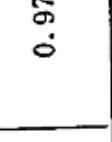
\includegraphics[max width=0.2\textwidth]{images/01912d0f-097c-7e75-8f32-4f326cd86c9f_95_250156.jpg} & 银白色金属, 柔软。 & 0.86 & 63.65 & 774 \\
\hline
咨 & Rb & 37 & 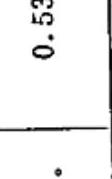
\includegraphics[max width=0.2\textwidth]{images/01912d0f-097c-7e75-8f32-4f326cd86c9f_95_250157.jpg} & 银白色金属, 柔软。 & 1. 532 & 38.89 & 688 \\
\hline
艳 & Cs & 55 & \includegraphics[max width=0.2\textwidth]{images/01912d0f-097c-7e75-8f32-4f326cd86c9f_95_250158.jpg} & 银白色金属,略带 金色光泽, 柔软。 & 1. 879 & 28.40 & 678.4 \\
\hline
\end{tabular}
}
\end{center}

注: 密度是指常温时的数据。

\begin{center}
\includegraphics[max width=0.7\textwidth]{images/01912d0f-097c-7e75-8f32-4f326cd86c9f_96_602232.jpg}
\end{center}

图 4-3 碱金属的原子和离子的大小示意图 (数据单位是 \({10}^{-{10}}\) 米)

碱金属原子的原子半径 \({}^{\left( 1\right) }\) 或离子半径一般都随着电子层数的增多而增大, 这是跟卤素和氧族元素的原子的变化相一致的。碱金属的熔点、沸点一般随着原子的电子层数的增加而降低。

\section*{二、焰色反应}

我们在炒菜的时候, 偶有食盐或食盐水溅在煤气火焰或煤火上, 火焰就呈现黄色。火焰呈现颜色的现象应用在科学实验上,可以检验一些金属或金属化合物。多种金属或它们的化合物在灼烧时使火焰呈特殊的颜色, 这在化学上叫做焰色反应。

[实验 4-7] 把装在玻璃棒上的铂丝 (也可用光洁无锈的铁丝或镍、铬、钨丝) 放在酒精灯火焰(最好用煤气灯, 火焰的本身颜色较微弱) 里灼烧, 等到跟原来的火焰颜色相同的时候, 用铂丝蘸碳酸钠溶液, 放在火焰上, 就可以看到火焰呈黄色(图 4-4)。每次试完后都要 用稀盐酸洗净铂丝, 在火焰上灼烧到没有什么颜色, 再分别蘸碳酸钾溶液、碳酸锂溶液作试验, 观察火焰的颜色。在观察钾的火焰颜色的时候, 要透过蓝色的钴玻璃

\customfootnote{

① 锂、钠、钾等金属的原子半径是指固态金属里两个邻近原子 核间的距离之半.

}

\begin{center}
\includegraphics[max width=0.5\textwidth]{images/01912d0f-097c-7e75-8f32-4f326cd86c9f_97_748791.jpg}
\end{center}

去观察, 这样就可以滤去黄色的 图 4-4 焰色反应试验的操作光, 避免碳酸钾里钠的杂质所造成的干扰。

碱金属和它们的化合物都能使火焰呈现出不同的颜色, 即呈现焰色反应。此外, 钙、锶、钡等金属也能呈现焰色反应。 根据焰色反应所呈现的特殊颜色, 可以测定金属或金属离子的存在。下面列出各金属或金属离子的焰色反应的颜色(并见封里彩图):

锂 紫红色

钠 黄色

钾 浅紫色(透过蓝色钴玻璃)

物 紫色

钙

锶 洋红色

钡 黄绿色

铜 绿色

在节日晚上燃放的五彩缤纷的焰火, 其中就有碱金属和锶、钡等金属的化合物所呈现的各种鲜艳色彩。

\section*{三、碱金属的化学性质}

我们知道,钠的化学性质很活泼。它的原子的最外电子层是一个电子, 在化学反应中容易失去。锂、钾、铷、铯等原子的最外电子层都是一个电子, 都容易失去, 因此它们的化学性质都很活泼。失去电子是氧化反应, 所以碱金属是强还原剂。

\section*{1. 跟非金属的反应}

碱金属跟卤素的反应, 有的是很剧烈的, 这我们已经知道了。

其它碱金属都象钠一样能跟氧气起反应。锂跟氧气起反应, 生成氧化锂。

\[
4\mathrm{{Li}} + {\mathrm{O}}_{2} = 2{\mathrm{{Li}}}_{2}\mathrm{O}
\]

钾、铷等跟氧气起反应, 生成比过氧化物更复杂的氧化物。

碱金属能够跟大多数的非金属起反应, 表现出很强的金属性。

\section*{2. 跟水的反应}

碱金属都跟水起反应, 生成氢氧化物并放出氢气。这类氢氧化物都能使酚酞溶液变红色。钾跟水的反应比钠更剧烈, 常使生成的氢气燃烧, 并发生轻微爆炸。

[实验 4-8] 从煤油里取出一块金属钾, 放在干燥玻璃片上, 用滤纸吸干煤油, 切取象绿豆大小那样的一块钾, 放在装冷水的烧杯里, 迅速用玻璃片盖好, 以免因轻微爆炸而飞溅出液体来。反应完成后滴入几滴酚酞溶液, 观察溶液颜色的变化。

\[
2\mathrm{\;K} + 2{\mathrm{H}}_{2}\mathrm{O} = 2\mathrm{{KOH}} + {\mathrm{H}}_{2} \uparrow
\]

这个反应就是钾原子失去一个电子, 水里的氢离子获得一个电子成为氢原子, 氢原子构成氢分子。

在这几种碱金属中, 由于原子的电子层数不同, 核对层数越多的电子的吸引力越小, 电子就越容易失去。随着原子的电子层数增加, 原子半径的增大, 碱金属的活动性增强。以钠和钾为例, 钾跟氧气、跟水的反应都比钠刷烈, 这些事实都可说明原子结构跟性质的关系。

\section*{囚、锂、钾、铷、铯的用途}

碱金属在生产和现代科学技术上都有一定的用途。锂用以制备有机化学工业上的催化剂、多种合金、高强度玻璃等。 锂还用于制热核反应的材料氚。钾的化合物象 \(\mathrm{{KCl}}\text{、}{\mathrm{K}}_{2}{\mathrm{{SO}}}_{4}\) 等是重要的肥料。铷和铯因在普通光的照射下能够放出电子, 用于制光电管等。

钾的许多重要化合物, 如氯化钾、硫酸钾、碳酸钾等都是钾肥。我们在初中化学里已学过钾肥的初步知识。土壤里钾的含量并不少, 但大部分以钾的矿物形式存在, 例如, 正长石、 白云母 \(\Phi\) 等等。这些矿物难溶于水,作物不能利用,只有在长期风化 (在土壤里受到空气、水分、酸的作用) 过程中, 才能逐步转化为作物可以吸收的水溶性的钾的化合物。因此, 土壤里的钾常常不能满足作物生长的需要, 人们往往要施用钾肥加以补充。

\customfootnote{

① 正长石: \({\mathrm{{KAlSi}}}_{3}{\mathrm{O}}_{43}\) 白云母: \({\mathrm{{KH}}}_{2}{\mathrm{{Al}}}_{3}{\mathrm{{Si}}}_{2}{\mathrm{O}}_{120}\) )

}

通常施用的钾肥主要是各种钾盐, 如氯化钾、硫酸钾、碳酸钾(草木灰的主要成分)等。这些钾盐都易溶于水, 在溶液里钾以离子形式存在, 易被作物吸收, 所以, 这些钾肥都是速效的。但必须注意的是, 由于它们易溶于水, 在施用时要防止雨水淋失。

在科学种田、夺取高产的过程中, 施用钾肥时, 要因地制宜, 注意氮、磷、钾三种肥料的合理配合。

\section*{习 题}

1. 试比较钠和钾的物理性质和化学性质。

2. 在卤族元素和碱金属元素中, 哪一族元素的原子比它们相应的离子小, 哪一族元素的原子比它们相应的离子大?试举例说明。

3. 写出下列反应的化学方程式。

(1) \({\mathrm{K}}_{2}\mathrm{O} + {\mathrm{H}}_{2}\mathrm{O} \rightarrow\)

(2) \({\mathrm{K}}_{2}{\mathrm{O}}_{2} + {\mathrm{H}}_{2}\mathrm{O} \rightarrow\)

(3) \({\mathrm{{Li}}}_{2}\mathrm{O} + {\mathrm{H}}_{2}\mathrm{O} \rightarrow\)

4. 用电子得失的观点来说明下列氧化-还原反应。

(1) \(2\mathrm{\;K} + {\mathrm{{Cl}}}_{2} = 2\mathrm{{KCl}}\)

(2) \(2\mathrm{\;K} + 2{\mathrm{H}}_{2}\mathrm{O} = 2\mathrm{{KOH}} + {\mathrm{H}}_{2} \uparrow\)

5. 把 4 克氢氧化钠溶解在水里, 制成溶液。这溶液能跟多少毫升的密度为 1.19 克/厘米 \({}^{3}\) 的盐酸起反应?

\section*{内容提要}

碱金属是一族金属元素,它们的原子结构的共同之点是次外层有 8 个电子 (锂是 2 个) 和最外电子层都只有一个电子, 在化学反应中容易失去电子, 因此, 它们的化学性质基本相似; 差别之处是核电荷数不同, 电子层数不同, 原子半径也不同, 因而碱金属元素的性质既相似又有差别。

碱金属的化学性质主要是强的金属性,随着原子半径的增大而金属性增强。它们的单质都是强还原剂。

\begin{center}
\includegraphics[max width=0.9\textwidth]{images/01912d0f-097c-7e75-8f32-4f326cd86c9f_101_648391.jpg}
\end{center}

碱金属和它们的化合物能使火焰呈现不同的颜色,即呈现焰色反应。根据焰色反应所呈现的特殊颜色,可以判断某些金属或金属离子的存在。

\section*{复习 题}

1. 回答下列问题:

(1)使用金属钠时为什么不能直接用手去拿, 而要用镊子去夹?

(2)观察钾的焰色时,为什么要透过蓝色的钴玻璃片?

(3)氢氧化钠固体或溶液为什么要保存在密闭容器里?

(4)钠和钾的外观很相似, 怎样来鉴别它们?

2. 钠和钾各 0.1 摩尔跟水起反应, 生成的氢氧化物的质量是否相等? 生成的氢气的质量是否相等?

3. 选择正确的答案填写在括号里。

(1) 下列哪些物质可用来制氧气: ( )

① \({\mathrm{{Na}}}_{2}{\mathrm{O}}_{2}\) , ② \({\mathrm{{CaCO}}}_{3}\) , ③ \({\mathrm{{KClO}}}_{3}\) ,

④ \({\mathrm{H}}_{2}{\mathrm{{SO}}}_{4}\) , ⑤ \({\mathrm{H}}_{2}\mathrm{O}\) 。

(2) 钠离子: ( )

① 遇水放出氢气, ② 要保存在煤油里,③ 比钠原子多 1 个电子, ④ 在无色火焰上灼烧显黄色。

(8) 下列哪些物质放在水里后, 溶液显碱性:( \(\;\) )

① \({\mathrm{{Na}}}_{2}{\mathrm{O}}_{2}\) , \(\because\) ② \(\mathrm{{NaCl}}\) , ③ \(\mathrm{{CuO}}\) , ④ \({}^{8}\mathrm{K}\) 。

4. 写出下列物质转化的化学方程式(其中的离子反应还要写出相应的离子方程式)。

\[
\mathrm{{Na}} \rightarrow {\mathrm{{Na}}}_{2}{\mathrm{O}}_{2} \rightarrow \underset{\begin{matrix} \rightarrow \\ \downarrow \end{matrix}}{\mathrm{{NaOH}}} \rightarrow {\mathrm{{Na}}}_{2}{\mathrm{{CO}}}_{2} \rightarrow {\mathrm{{CaCO}}}_{3} \rightarrow \mathrm{{Ca}}{\left( {\mathrm{{HCO}}}_{3}\right) }_{2}
\]

\section*{》小姐、【}

的不同性能的广流和多式和平方中。 (不断加强能夜留《指待》的代表“我家老成家”,不知道,可知如果他在 \({\mu }_{k}\left( {t,0}\right) = \left( {1 - t}\right) \left( {t,0}\right) ,\;{t}_{k}^{\left( 0\right) }\left( {t,0}\right) = \left( {1 - t}\right) \left( {t,0}\right) - \left( {1 - t}\right) \left( {t,0}\right) ,\;t \in \left\lbrack {0,1}\right\rbrack .\) 清心何可以忘。是在这种感受了自己的人的不是概率越来越 。 * 如何在所有的 \(M\left( {t{k}^{\prime }}\right)\) 上,这些分别是如果 \({W}^{\prime }\) the integral contraction on the integrated to the context

the component of the component of the component of the component

the field \(T\) and the component of the component of the

\section*{第五章 原子结构 元素周期律}

到目前为止, 我们已经学习了氧、惰性气体、氢、碳、卤族、 氧族、碱金属等元素和它们的一些化合物, 知道元素、化合物的性质跟它们的结构有密切的关系。只有了解了它们的结构, 才能深刻地认识它们的性质和变化规律。所以, 我们要在初中学习的物质结构初步知识的基础上, 进一步学习物质结构的知识。本章我们先来学习有关原子结构和反映元素内在联系的元素周期律的知识。至于物质结构的其它知识, 以后将要逐步学习。

\section*{第一节 原子 核}

\section*{一、原子核}

原子是由居于原子中心的带正电的原子核和核外带负电的电子构成的。由于原子核带的电量跟该外电子的电量相等而电性相反, 因此, 原子作为一个整体不显电性。原子很小, 而原子核更小, 它的半径约是原子的万分之一, 它的体积只占原子体积的几千亿分之一。原子核由质子和中子构成。每个质子带一个单位正电荷, 中子呈电中性, 因此, 核电荷数由质子数决定。核电荷数的符号为 \(Z\) 。

核电荷数 \(\left( Z\right) =\) 核内质子数 \(=\) 核外电子数

质子的质量为 \({1.6726} \times {10}^{-{27}}\) 千克,中子的质量稍大些, 为 \({1.6748} \times {10}^{-{27}}\) 千克,电子的质量很小,仅约为质子质量的 \(1/{1836}\) ,所以,原子的质量主要集中在原子核上。由于质子、 中子的质量很小, 计算不方便, 因此, 通常用它们的相对质量。

通过科学实验测得, 作为原子量标准的那种碳原子的质量是 \({1.9927} \times {10}^{-{26}}\) 千克,它的 \(1/{12}\) 为 \({1.6606} \times {10}^{-{27}}\) 千克。 质子和中子对它的相对质量分别为 1.007 和 1.008 , 取近似整数值为 1 。显然, 如果忽略电子的质量, 将原子核内所有的质子和中子的相对质量取近似整数值加起来, 所得的数值, 叫做质量数,用符号 \(A\) 表示。中子数用符号 \(N\) 表示。则

质量数 \(\left( A\right) =\) 质子数 \(\left( Z\right) +\) 中子数 \(\left( N\right)\)

因此, 只要知道上述三个数值中的任意两个, 就可以推算出另一个数值来。例如, 知道硫原子的核电荷数为 16 , 质量数为 32 , 则

硫原子的中子数 \(= A - Z = {32} - {16} = {16}\)

归纳起来,如以 \({}_{2}^{A}X\) 代表一个质量数为 \(A\) 、质子数为 \(Z\) 的原子, 那么, 组成原子的粒子间的关系可以表示如下:

原子 \(\left( {{}_{Z}^{A}X}\right) \left\{ \begin{array}{l} \text{ 原子核 }\left\{ \begin{array}{ll} \text{ 质子 } & Z\text{ 个 } \\ \text{ 中子 } & \left( {A - Z}\right) \text{ 个 } \end{array}\right. \\ \text{ 核外电子 }\;Z\text{ 个 } \end{array}\right.\)

\section*{二、同位素}

我们已经知道, 具有相同核电荷数 (即质子数) 的同一类原子叫做元素。也就是说, 同种元素的原子的质子数相同, 那么, 它们的中子数是否相同呢? 科学研究证明, 不一定相同。 例如, 氢元素的原子都含 1 个质子, 但有的氢原子不含中子, 有的氢原子含 1 个中子,还有的氢原子含 2 个中子:

不含中子的氢原子叫做氕;

含 1 个中子的氢原子叫做氘, 就是重氢;

含 2 个中子的氢原子叫做氚 \(\text{①}\) , 就是超重氢。

为了便于区别,将氕记为 \({}_{1}^{1}\mathrm{H}\) ,氘记为 \({}_{1}^{2}\mathrm{H}\) (或 D),氚记为 \({}_{1}^{3}\mathrm{H}\) (或 T)。元素符号的左下角记核电荷数, 左上角记质量数。

人们把原子里具有相同的质子数和不同的中子数的同一元素的原子互称同位素。许多元素都有同位素。上述 \({}_{1}^{1}\mathrm{H}\text{、}{}_{1}^{2}\mathrm{H}\) 、 \({}_{1}^{3}\mathrm{H}\) 是氢的三种同位素, \({}_{1}^{2}\mathrm{H}\text{、}{}_{1}^{3}\mathrm{H}\) 是制造氢弹的材料。铀元素有 \({}_{92}^{234}\mathrm{U}\text{、}{}_{92}^{235}\mathrm{U}\text{、}{}_{92}^{238}\mathrm{U}\) 等多种同位素, \({}_{92}^{235}\mathrm{U}\) 是制造原子弹的材料和核反应堆的燃料。碳元素有 \({}_{6}^{12}\mathrm{C}\text{、}{}_{6}^{12}\mathrm{C}\) 和 \({}_{6}^{14}\mathrm{C}\) 等几种同位素, 而 \({}_{4}^{12}\mathrm{C}\) 就是我们将它的质量的 \(1/{12}\) 当做原子量标准的那种碳原子。同一元素的各种同位素虽然质量数不同, 但它们的化学性质几乎完全相同。在天然存在的某种元素里, 不论是游离态还是化合态, 各种同位素所占的原子百分比一般是不变的。我们平常所说的某种元素的原子量, 是按各种天然同位素原子所占的一定百分比算出来的平均值。例如, 元素氯是 \({}_{17}^{85}\mathrm{{Cl}}\) 和 \({}_{17}^{37}\mathrm{{Cl}}\) 两种同位素的混和物,从下列数据即可计算出氯元素的原子量:

符号 同位素的原子量 在自然界各同位素

原子的百分组成

34.969 75.77

36.966

\({34.969} \times {0.7577} + {36.966} \times {0.2423} = {35.453}\)

① 一只音 pio, 氘音 dao, 氚音 chuan。 即氯的原子量为 35.453 。

同理, 根据同位素的质量数, 也可以算出近似原子量。

\section*{习 题}

1. 下列说法是否正确? 如有错误, 加以改正。

(1)石墨和金刚石是由碳元素组成的两种同位素。

(2) 人们已经知道了 107 种元素,就是说人们已经知道了 107 种原子。

2. 指出下列各原子中质子、中子、电子的数目各是多少:

\({}^{12}\mathrm{C},{}^{13}\mathrm{C},{}^{18}\mathrm{O},{}^{17}\mathrm{O},{}^{18}\mathrm{O},{}^{18}\mathrm{F},{}^{24}\mathrm{{Mg}},\)

\({}_{19}^{39}\mathrm{\;K},\;{}_{19}^{40}\mathrm{\;K},\;{}_{19}^{41}\mathrm{\;K},\;{}_{20}^{40}\mathrm{{Ca}},\;{}_{20}^{42}\mathrm{{Ca}}\) 。

3. 氧有三种天然同位素, 它们的同位素原子量和各同位素原子的百分组成数据分列如下:

\({}^{1}{}_{8}^{6}\mathrm{O}\;{15.994915}\;{99.759}\%\)

\({}_{8}^{17}\mathrm{O}\;{16.999133}\) \({0.037}\%\)

180 17.99916

计算氧元素的原子量。

4. 镁有三种天然同位素: \({}_{12}^{24}\mathrm{{Mg}}\) (占 \({78.7}\%\) ), \({}_{12}^{25}\mathrm{{Mg}}\) (占 \({10.13}\%\) ), \({}_{12}^{26}\mathrm{{Mg}}\) (占 \({11.17}\%\) ), 计算镁元素的近似原子量。

\section*{第二节 核外电子的运动状态}

电子带负电荷,质量很小,仅 \({9.1095} \times {10}^{-{31}}\) 千克。它在原子这样大小的空间 (直径约 \({10}^{-{10}}\) 米) 内运动,速度很快,接近光速 \(\left( {3 \times {10}^{8}}\right.\) 米 \(/\) 秒 \()\) 。电子的运动情形跟质量大、速度小的普通物体是否相同? 有没有特殊的规律? 现在我们就来进行研究。

\section*{一、电子云}

我们在生活中见到汽车在公路上奔驰,用仪器观察到人造卫星按一定轨道围绕地球旋转, 都可以测定或根据一定的数据计算出它们在某一时刻所在的位置,并描画出它们的运动轨迹。但是, 核外电子的运动规律就跟上述普通物体不同。 核外电子的运动没有上述那样确定的轨道, 我们不能测定或计算出它在某一时刻所在的位置, 也不能描画它的运动轨迹。 我们在描述核外电子运动时,只能指出它在原子核外空间某处出现机会的多少。电子在核外空间一定范围内出现, 好象带负电荷的云雾笼罩在原子核周围, 所以我们形象地称它为“电子云”。为了便于理解, 我们用给氢原子照像的比喻来加以说明。我们知道, 氢原子核外有一个电子。为了在一瞬间找到电子在氢原子核外的确定位置, 我们假想有一架特殊的照相机, 可以用它来给氢原子照相。先给某个氢原子拍五张照片, 得到如图 5-1 所示的不同的图象。图 5-1 里④表示原子核, 一个

\begin{center}
\includegraphics[max width=1.0\textwidth]{images/01912d0f-097c-7e75-8f32-4f326cd86c9f_107_547413.jpg}
\end{center}

图 5-1 氢原子的五次瞬间照相

小黑点表示电子在这里出现过一次。然后继续给氢原子拍上成千上万张照片, 并把这些照片一一对比研究, 这样, 我们就获得一个印象: 电子好象是在氢原子核外作毫无规律的运动, 一会儿在这里出现, 一会儿在那里出现。如果我们将这些照片叠印, 就会看到如图 5-2 所示的图象。图象说明, 对氢原子的照片叠印张数越多, 就越能使人形成一团电子云雾笼罩原子核的印象, 而这团 “电子云雾” 呈球形对称, 在离核越近处密度越大, 离核越远处密度越小。也就是说, 在离核越近处单位体积的空间中电子出现的机会越多,离核越远处单位体积的空间中电子出现的机会越少。实际上,图 5-2(d) 就是在通常状况下氢原子的电子云示意图。

\begin{center}
\includegraphics[max width=1.0\textwidth]{images/01912d0f-097c-7e75-8f32-4f326cd86c9f_108_831895.jpg}
\end{center}

图 5-2 将若干张氢原子瞬间照相叠印的结果

\section*{二、核外电子的运动状态}

\section*{1. 电子层}

我们已经知道, 在含有多个电子的原子里, 电子的能量并不相同。能量低的, 通常在离核近的区域运动; 能量高的, 通常在离核远的区域运动。根据电子的能量差异和通常运动的区域离核的远近不同, 可以将核外电子分成不同的电子层。

我们怎么知道含有多个电子的原子里核外电子的能量并不相同呢? 根据对元素电离能数据的分析, 可以初步得到这个结论。

什么是电离能? 从气态原子 (或气态阳离子) 中去掉电子, 把它变成气态阳离子 (或更高价的气态阳离子), 需要克服核电荷的引力而消耗能量,这个能量叫做电离能,符号为 \(I\) ,单位常用电子伏特 \({}^{\left( 1\right) }\) 。

从元素的气态原子去掉一个电子成为 +1 价气态阳离子所需消耗的能量,称为第一电离能 \(\left( {I}_{1}\right)\) ; 从 +1 价气态阳离子再去掉一个电子成为 +2 价气态阳离子所需消耗的能量, 叫做第二电离能 \(\left( {I}_{2}\right)\) ; 依次类推。

表 5-1 列出了几种元素电离能的数据。

表 5-1 几种元素的电离能(电子伏特)

\begin{center}
\adjustbox{max width=\textwidth}{
\begin{tabular}{|c|c|c|c|c|c|c|c|c|c|c|}
\hline
核电 荷数 & 元素 符号 & \({I}_{1}\) & \({I}_{2}\) & \({I}_{3}\) & \({I}_{4}\) & \({I}_{5}\) & \({I}_{6}\) & \({I}_{7}\) & \({I}_{8}\) & \({I}_{9}\) \\
\hline
3 & Li & 5.4 & 75.6 & 122.4 & \phantom{X} & \phantom{X} & \phantom{X} & \phantom{X} & \phantom{X} & \phantom{X} \\
\hline
4 & Be & 9.3 & 18.2 & 153.9 & 217.7 & \phantom{X} & \phantom{X} & \phantom{X} & \phantom{X} & \phantom{X} \\
\hline
5 & B & 8.3 & 25.1 & 37.9 & 259. 3 & 340.1 & \phantom{X} & \phantom{X} & \phantom{X} & \phantom{X} \\
\hline
6 & C & 11.3 & 24.4 & 47.9 & 64.5 & 392.0 & 489. 8 & \phantom{X} & \phantom{X} & \phantom{X} \\
\hline
7 & N & 14.5 & 29. 6 & 47.4 & 77.5 & 97.9 & 551.9 & 666. 8 & \phantom{X} & \phantom{X} \\
\hline
8. & O & 13.6 & 35.1 & 54.9 & 77.4 & 113.9 & 138.1 & 739. 1 & 871.1 & \phantom{X} \\
\hline
9 & \(\mathrm{F}\) & 17.4 & 35.0 & 62.6 & 87.1 & 114.2 & 157.1 & 185.1 & 953. 6 & 1102 \\
\hline
\end{tabular}
}
\end{center}

① 电子伏特是一个电子在真空中通过 1 伏特电位差所获得的 动能, 它是一种描述微观粒子运动的能量单位。

1 电子伏特 \(= {1.6022} \times {10}^{-{19}}\) 焦耳。

从表上数据可见, 元素的第二电离能大于第一电离能, 第三电离能大于第二电离能,依次类推,即 \({I}_{1} < {I}_{2} < {I}_{3} < \cdots \cdots\) 。 这是容易理解的, 因为从 +1 价气态阳离子中去掉一个电 子需克服的电性引力比从中性原子去掉一个电子要大, 消耗的能量要多。同理, 从 +2 价气态阳离子中去掉一个电子, 需克服的电性引力, 比从 +1 价气态阳离子中去掉一个电子更大, 消耗的能量更多。因此, 一个原子的电离能是依次增大, 甚至是成倍增长的, 但增大的倍数并不相同。有的增大得不多, 有的增大得很多。我们在表 5-1 上将增大倍数很多的电离能数据前面和下面标上粗线, 以示区别。下面就来分析这些数据。

\(\mathrm{{Li}}\) ,原子核外有 3 个电子。 \({I}_{3}\) 比 \({I}_{2}\) 增大不到一倍,但 \({I}_{2}\) 比 \({I}_{1}\) 却增大了十几倍。这说明什么问题? 说明这 3 个电子可分为两组,两组能量有差异。 \({I}_{1}\) 比 \({I}_{2}\text{、}{I}_{3}\) 小得多,说明有一个电子能量较高, 通常在离核较远的区域运动, 容易被去掉。 另外两个电子能量较低, 通常在离核较近的区域运动。

Be,原子核外有 4 个电子。按照如上的分析, \({I}_{2}\) 比 \({I}_{1},{I}_{4}\) 比 \({I}_{3}\) 均增大不到一倍,但 \({I}_{3}\) 比 \({I}_{2}\) 却增大了好几倍。因此可以认为有两个电子能量较低, 通常在离核较近的区域运动; 另外两个电子能量较高, 通常在离核较远的区域运动。

分析 \(\mathrm{B}\text{、}\mathrm{C}\text{、}\mathrm{N}\text{、}\mathrm{O}\text{、}\mathrm{F}\) 等元素的电离能的数据,将会发现它们的核外电子都分两组, 第一组是两个电子, 能量较低, 通常在离核较近的区域运动; 第二组分别是 \(3\text{、}4\text{、}5\text{、}6\text{、}7\) 个电子,能量较高, 通常在离核较远的区域运动。

如果分析其它元素的电离能数据, 也会得出相似的结论。 可见, 在含多个电子的原子中, 电子是分层排布的。

\section*{2. 电子亚层和电子云的形状}

科学研究发现, 在同一电子层中, 电子的能量还稍有差别, 电子云的形状也不相同。根据这个差别, 又可以把一个电子层分成一个或几个亚层,分别用 \(s\text{、}p\text{、}d\text{、}f\) 等符号 \(\Phi\) 表示。 \(\mathrm{K}\) 层只包含一个亚层,即 \(s\) 亚层; \(\mathrm{L}\) 层包含两个亚层,即 \(s\) 亚层和 \(p\) 亚层; \(\mathrm{M}\) 层包括三个亚层,即 \(s\text{、}p\text{、}d\) 亚层; \(\mathrm{N}\) 层包括四个亚层,即 \(s\text{、}p\text{、}d\text{、}f\) 亚层。不同亚层的电子云形状不同。 \(s\) 亚层的电子云是以原子核为中心的球形, \(p\) 亚层的电子云是 纺锤形, \(d\) 亚层、 \(f\) 亚层的电子云形状比较复杂,这里就不介绍了。

在同一个电子层里,亚层电子的能量是按 \(s\text{、}p\text{、}d\text{、}f\) 的次序递增的。为了清楚地表示某个电子处于核外哪个电子层和亚层 (自然同时也表示 它的能量高低和电子云的形状), 可将电子层的序数 \(n\) 标在亚层符号的前面。如处于 \(\mathbf{K}\) 尽 \(的\mathbf{s}\) 亚层的电子标为 \({1s}\) ; 处于 \(\mathrm{L}\) 层的 \(s\) 亚层和 \(p\) 亚层的电子标为 \({2s}\) 和 \({2p}\) ; 处于 \(\mathrm{M}\) 层的 \(d\) 亚层的电子标为 \({3d}\) ; 处于 \(\mathrm{N}\) 层的 \(f\) 亚层的电子标为 \({4f}\) 。图 5-3a 就是氢的 \({1s}\) 电子云。

\begin{center}
\includegraphics[max width=1.0\textwidth]{images/01912d0f-097c-7e75-8f32-4f326cd86c9f_111_261347.jpg}
\end{center}

图 5-3 氢原子的 \({1s}\) 电子云

\customfootnote{

① \(s\text{、}p\text{、}d\text{、}f\) 是光谱学上的符号。

}

图 5-3b 虚线表示的球壳称为电子云的界面。在界面内电子出现的机会最多, 界面外电子出现的机会很少。通常也用电子云界面图来表示电子云。图 5-3c 是氢原子 \({1s}\) 电子云的界面图, 它把表示电子出现机会的小黑点略去了。

\section*{3. 电子云的伸展方向}

电子云不仅有确定的形状,而且有一定的伸展方向。 \(s\) 电子云是球形对称的, 在空间各个方向上伸展的程度相同。2p 电子云如图 5-4 所示, 在空间可以有三种互相垂直的伸展方向。 \(d\) 电子云可以有五种伸展方向, \(f\) 电子云可以有七种伸展方向。

\begin{center}
\includegraphics[max width=1.0\textwidth]{images/01912d0f-097c-7e75-8f32-4f326cd86c9f_112_942620.jpg}
\end{center}

图 5-4 \({2p}\) 电子云的三种伸展方向

如果把在一定的电子层上, 具有一定的形状和伸展方向的电子云所占据的空间称为一个轨道,那么 \(s\text{、}p\text{、}d\text{、}f\) 四个亚层就分别有 \(1\text{、}3\text{、}5\text{、}7\) 个轨道。这样,各电子层可能有的最多轨道数如下:

\[
n = 2\;s\text{、}p\;1 + 3 = 4 = {2}^{2}
\]

\[
n = 3\;s\text{、}p\text{、}d\;1 + 3 + 5 = 9 = {3}^{2}
\]

\[
n = 4\;s\text{、}p\text{、}d\text{、}f\;1 + 3 + 5 + 7 = {16} = {4}^{2}
\]

\[
{n}^{2}
\]

即每个电子层可能有的最多轨道数应为 \({n}^{2}\) 。

\section*{4. 电子的自旋}

电子不仅在核外空间不停地运动, 而且还作自旋运动。电子自旋有两种状态, 相当于顺时针和逆时针两种方向。平常我们用向上箭头 \(\uparrow\) 和向下箭头 \(\downarrow\) 来表示不同的自旋状态。

通过以上的叙述我们可以看出, 电子在原子核外的运动状态是相当复杂的, 必须由它所处的电子层、电子亚层、电子云的空间伸展方向和自旋状态四个方面来决定。前三个方面跟电子在核外空间的位置有关, 体现了电子在核外空间的运动状态, 确定了电子的轨道。因此, 当我们要说明一个电子的运动状态时,必须同时指明它处于什么轨道和哪一种自旋状态。

\section*{习 题}

1. 你如何理解电子层、电子亚层和电子云这三个概念? 氢原子核外只有一个电子, 为什么要用电子云来描述它的运动?

2. 什么叫电离能?为什么根据元素电离能的变化可以判断核外电子是分层排布的?

3. 原子核外电子的运动状态,必须从哪几个方面来进行描述?

4. \({1s}\text{、}{2p}\text{、}{3d}\text{、}{4f}\) 各表示什么意思?

5. \(d\) 亚层和 \(f\) 亚层各有多少轨道? 在同一轨道上运动的电子可以有几种不同的运动状态?

6. \(2{p}_{x}\text{、}2{p}_{y}\text{、}2{p}_{z}\) 各表示什么意思?

\section*{第三节 原子核外电子的排布}

上一节我们学习了原子核外电子的运动状态, 了解电子是分层排布的, 而电子层又可分为几个电子亚层。现在, 我们就来进一步讨论原子核外电子的排布规律。

\section*{一、泡利①不相容原理}

我们先来讨论锂的核外电子排布。锂原子有 3 个电子。 这 3 个电子是都在一个轨道上, 还是分别在几个轨道上呢? 实验证明,有 2 个在 \({1s}\) 轨道上,1 个在 \({2s}\) 轨道上。在 \({1s}\) 轨道上的 2 个电子自旋方向是平行的, 还是相反的? 实验证明, 是相反的。在 \({2s}\) 轨道上的那个电子虽然自旋方向跟 \({1s}\) 轨道上的一个电子相同,但它们分别处于两个不同的轨道。其它元素核外电子排布有类似的情况。

从以上建立在实验基础上的讨论中我们看到, 在原子核外电子的排布中, 排在同一轨道上的两个电子, 自旋方向就相反; 而自旋方向相同的电子, 必然处于不同的轨道上。我们知道, 一个轨道是由电子层、电子亚层和电子云的伸展方向三方面确定的, 因此, 可以得出一个结论: 在同一个原子里; 没有运动状态四个方面完全相同的电子存在。这个结论是泡利提出来的, 叫做泡利不相容原理。

根据这个原理, 我们可以推算出各电子层可以容纳的最多电子数。我们知道,每个电子层可能有的最多轨道数为 \({n}^{2}\) , 而每个轨道又只能容纳 2 个电子, 因此, 各电子层可能容纳的电子总数就是 \(2{n}^{2}\) 。现将 1-4 电子层可容纳电子的最大数目列于表 5-2 中。

\customfootnote{

① 泡利(Pauli,1900-1958),臭地利物理学家。

}

表 5-2 1-4 电子层可容纳电子的最大数目

\begin{center}
\adjustbox{max width=\textwidth}{
\begin{tabular}{|c|c|c|c|c|c|c|c|c|c|c|}
\hline
电 子 层 ( \(n\) ) & K (1) & \multicolumn{2}{|c|}{L (2)} & \multicolumn{3}{|c|}{M (3)} & \multicolumn{4}{|c|}{\(\mathrm{N}\) (4)} \\
\hline
电子 \(亚\) 层 & 8 & 8 & p & 8 & \(p\) & \(d\) & 8 & P & \(d\) & \(f\) \\
\hline
亚层中的轨道数 & 1 & 1 & 3 & 1 & 3 & 5 & 1 & 3 & 5 & 7 \\
\hline
亚层中的电子数 & 2 & 2 & 6 & 2 & 6 & 10 & 2 & 6 & 10 & 14 \\
\hline
每个电子层中可容纳 电子的最大数目 & 2 & \multicolumn{2}{|c|}{8} & \multicolumn{3}{|c|}{18} & \multicolumn{4}{|c|}{32} \\
\hline
\end{tabular}
}
\end{center}

\section*{二、能量最低原理}

生活常识告诉我们, 水总是由高处向低处流, 山上的石头可以自动地向山下滚。这是由于物体处于高势能状态时不如低势能状态稳定。同理, 在核外电子的排布中, 通常状况下电子也总是尽先占有能量最低的轨道, 只有当这些轨道占满后, 电子才依次进入能量较高的轨道。这个规律叫做能量最低原理。

那么, 哪些轨道的能量高, 哪些轨道的能量低呢?

我们知道, 不同电子层具有不同的能量, 而每个电子层中不同亚层的能量也不相同。为了表示原子中各电子层和亚层电子能量的差异, 人们把原子中不同电子层和亚层的电子按能量高低排成顺序,象台阶一样,叫做能级。例如, \({1s}\) 能级, \({2s}\) 能级, \({2p}\) 能级,等等。在一个原子中,离核越近、 \(n\) 越小的电子层能量越低。在同一电子层中,各亚层的能量是按 \(s\text{、}p\) 、 \(d\text{、}f\) 的次序增高的。因此,我们可以认为 \({2s}\) 能级高于 \({1s}\) 能级, \({2p}\) 能级高于 \({2s}\) 能级,等等。可是对于那些核外电子数较多的元素来说, 情况就比较复杂了。为什么呢? 因为多电子原子的各个电子之间存在着排斥力, 在研究某个外层电子的运动状态时, 必须同时考虑到核对它的吸引力及其它电子对它的排斥力。由于其它电子的存在, 往往减弱了原子核对外层电子的吸引力, 从而使多电子原子的电子所处的能级产生了交错现象。图 5-5 是多电子原子电子的近似能级图, 图上一个方框代表一个轨道。

\begin{center}
\includegraphics[max width=0.7\textwidth]{images/01912d0f-097c-7e75-8f32-4f326cd86c9f_116_160371.jpg}
\end{center}

图 5-5 多电子原子电子的近似能级图

从图 5-5 可以看到, 从第三电子层起就有能级交错现象, 例如, \({3d}\) 电子的能量似乎应该低于 \({4s}\) ,而实际上 \({E}_{4d} > {E}_{4s}\) 。按照能量最低原理,电子在进入核外电子层时,不是排完了 \({3p}\) 就排 \({3d}\) ,而是先排 \({4s}\) 。排完了 \({4s}\) ,才排 \({3d}\) 。

应用多电子原子电子的近似能级图, 并根据能量最低原理, 就可以确定电子排入各轨道的次序, 如图 5-6 所示。

\begin{center}
\includegraphics[max width=0.5\textwidth]{images/01912d0f-097c-7e75-8f32-4f326cd86c9f_117_447446.jpg}
\end{center}

图 5-6 电子填入轨道的顺序

\section*{三、洪特①规则}

我们运用泡利不相容原理和能量最低原理, 再来讨论碳、 氮、氧三种元素原子的核外电子的排布情况。

\customfootnote{

① 洪特(Hund, 1896-), 德国物理学家。

}

碳元素的核电荷数为 6 , 即核外有 6 个电子。根据上述两个原理,核外电子首先在 \({1s}\) 轨道排入两个自旋方向相反的电子,然后另 2 个自旋方向相反的电子排入 \({2s}\) 轨道,还剩 2 个电子,应排入 \({2p}\) 轨道。 \({2p}\) 轨道有 3 个,它们是以自旋方向相反的方式排入一个 \({2p}\) 轨道,还是以自旋方向相同的方式排入两个 \({2p}\) 轨道呢? 人们从科学实验中总结出的叫做 洪 特规则的一条规律回答了这个问题, 这个规则指出, 在同一亚层中的各个轨道 (如 3 个 \(p\) 轨道,或 5 个 \(d\) 轨道,或 7 个 \(f\) 轨道) 上, 电子的排布尽可能分占不同的轨道, 而且自旋方向相同, 这样排布整个原子的能量最低。因此, 碳、氮、氧三元素原子的电子层排布应该如图 5-7 所示。图中 \(\left| \frac{1s}{ \uparrow \downarrow }\right| \frac{2s}{\left( { \uparrow \downarrow }\right) \left| \uparrow \right| \uparrow }\frac{2p}{ \uparrow \uparrow }\) 叫做轨道表示式,一个方框表示一个轨道; 式子 \(1{s}^{2}2{s}^{2}2{p}^{2}\) 叫做电子排布式, 式中右上角的数字表示该轨道中电子的数目,如 \(1{s}^{2}\) 表示在 \({1s}\) 轨道上有两个电子。

\begin{center}
\includegraphics[max width=0.9\textwidth]{images/01912d0f-097c-7e75-8f32-4f326cd86c9f_118_325547.jpg}
\end{center}

图 5-7 碳、氮、氧原子的电子层排布

根据上述三个原理和多电子原子电子的近似能级图, 我们将核电荷数为 1-36 的元素原子的核外电子的排布情况列入表 5-3 中。

表 5-3 核电荷数为 \(1 \rightharpoonup {36}\) 的元素的电子层排布

\begin{center}
\adjustbox{max width=\textwidth}{
\begin{tabular}{|c|c|c|c|c|c|c|c|c|c|c|c|c|c|c|c|c|c|}
\hline
\phantom{X} & \multirow{3}{*}{核电荷数} & \multirow{3}{*}{元素符号} & \multicolumn{5}{|c|}{电子 ` ` ` `} & \multirow{3}{*}{核电荷数} & \multirow{3}{*}{元 素 符 号} & \multicolumn{8}{|c|}{电 子 层} \\
\cline{1-1}
\cline{4-8}
\cline{11-18}
\phantom{X} & & & \({\mathbf{K}}_{1}\) & \multicolumn{2}{|c|}{L.} & M & N & & & \(\mathbf{K}\) & \multicolumn{2}{|c|}{L} & \multicolumn{3}{|c|}{M} & \multicolumn{2}{|c|}{N} \\
\cline{1-1}
\cline{4-8}
\cline{11-18}
\phantom{X} & & & 1s & \phantom{X} & \({2s} \cdot {2p}\) & \({3s}\;{3p}\;{3d}\) & 48 4p & & & 1s & 2.8 & \({2p}\) & 3s & 3 p & \({3d}\) & \phantom{X} & 48 4p \\
\hline
\phantom{X} & 1 & H & 1 & \phantom{X} & \phantom{X} & \phantom{X} & \phantom{X} & 19 & K & 2 & 2 & 6 & 2 & 6 & \phantom{X} & 1 & \phantom{X} \\
\hline
\phantom{X} & 2 & He & 2 & \phantom{X} & \phantom{X} & \phantom{X} & \phantom{X} & 20 & Ca & 2 & \(2\) . & 6 & 2 & 6 & \phantom{X} & 2 & \phantom{X} \\
\hline
\phantom{X} & 3 & Li & 2 & 1 & \phantom{X} & \phantom{X} & \phantom{X} & 21 & Sc & 2 & 2 & 6 & 2 & 6 & 1 & 2 & \phantom{X} \\
\hline
\phantom{X} & 4 & Be & 2 & 2 & \phantom{X} & \phantom{X} & \phantom{X} & 22 & Ti & 2 & 2 & 6 & 2 & 6 & 2 & 2 & \phantom{X} \\
\hline
, & 5 & B & 2 & 2 & 1 & \phantom{X} & \phantom{X} & 23 & v & 2 & 2 & 6 & 2 & 6 & 3 & 2 & \phantom{X} \\
\hline
\phantom{X} & 6 & C & 2 & 2 & 2 & \phantom{X} & \phantom{X} & 24 & Cr & 2 & 2 & 6 & 2 & 6 & ,5 & 1 & \phantom{X} \\
\hline
\phantom{X} & 7 & N & 2 & 2 & 3 & \phantom{X} & \phantom{X} & 25 & Mn & 2 & 2 & 6 & 2 & 6 & 5 & 2 & \phantom{X} \\
\hline
\phantom{X} & 8 & O & 2 & 2 & 4 & \phantom{X} & \phantom{X} & 26 & Fe & 2 & 2 & 6 & 2 & 6 & 6 & 2 & \phantom{X} \\
\hline
\phantom{X} & )9 & F & 2 & 2 & 5 & \phantom{X} & \phantom{X} & 27 & Co & 2 & 2 & 6 & 2 & 6 & 7 & 2 & \phantom{X} \\
\hline
\phantom{X} & 10 & Ne & 2 & 2 & 6 & \phantom{X} & \phantom{X} & 28 & Ni & 2 & 2 & 6 & 2 & 6 & 8 & 2 & \phantom{X} \\
\hline
\phantom{X} & 11 & Na & 2 & 2 & 6 & 1 & \phantom{X} & 29 & Cu & 2 & 2 & 6 & 2 & 6 & 10 & 1 & \phantom{X} \\
\hline
\phantom{X} & 12 & Mg & 2 & 2 & 6 & 2 & \phantom{X} & 30 & Zn & 2 & 2 & 6 & 2 & 6 & 10 & 2 & 1 \\
\hline
\phantom{X} & 13 & A1 & 2 & 2 & 6 & 21 & \phantom{X} & 31 & Ga & 2 & 2 & 6 & 2 & 6 & 10 & 2 & 1 \\
\hline
\phantom{X} & 14 & Si & 2 & 2 & 6 & 22 & \phantom{X} & 32 & Ge & 2 & 2 & 6 & 2 & 6 & 10 & 2 & 2 \\
\hline
\phantom{X} & 15 & P & 2 & 2 & 6 & 23 & \phantom{X} & 33 & As & 2 & 2 & 6 & 2 & 6 & 10 & 2 & 3 \\
\hline
\phantom{X} & - 16 & S & 2 & 2 & 6 & 24 & \phantom{X} & 34 & Se & 2 & 2 & 6 & 2 & 6 & 10 & 2 & 4 \\
\hline
\phantom{X} & 17 & Cl & 2 & 2 & 6 & 25 & \phantom{X} & 35 & Br & 2 & 2 & 6 & 2 & 6 & 10 & 2 & 5 \\
\hline
\phantom{X} & \({18} =\) & Ar & 2 & 2 & 6 & 26 & \phantom{X} & 36 & \(\mathrm{{Kr}}\) & 2 & 2 & 6 & 2 & 6 & 10 & 2 & 6 \\
\hline
\end{tabular}
}
\end{center}

从表上可以看出, 核电荷数为 24 的元素 \(\mathrm{{Cr}}\) ,核电荷数为 29 的元素 \(\mathrm{{Cu}}\) ,它们的电子层结构并没有完全按照前述规律排布, \(\mathrm{{Cr}}\) 和 \(\mathrm{{Cu}}\) 在排了 \(3{p}^{6}\) 后似应排成 \(3{d}^{4}4{s}^{2}\) 和 \(3{d}^{9}4{s}^{2}\) ,但实验数据表明应排成 \(3{d}^{5}4{s}^{1}\) 和 \(3{d}^{10}4{s}^{1}\) ; 其它元素的电子层排布也有类似的情况。根据这种情况, 人们又归纳出一条规律, 就是对于同一电子亚层, 当电子排布为全充满、半充满或全空时, 是比较稳定的。即

全充满 \({p}^{6}\) 或 \({d}^{10}\) 或 \({f}^{14}\)

半充满 \(\;{p}^{8}\) 或 \({d}^{5}\) 或 \({f}^{7}\)

全 空 \({p}^{0}\) 或 \({d}^{0}\) 或 \({f}^{0}\)

这是洪特规则的一种特例。上述 \(\mathrm{{Cr}}\text{、}\mathrm{{Cu}}\) 的电子层排布,就是属于 \(d\) 轨道半充满、全充满时比较稳定的例子。

这里需要指出, 核外电子的排布情况是通过实验测定的。 上面讲的泡利不相容原理、能量最低原理和洪特规则三条原理, 是从大量事实中概括出来的, 它们能帮助我们了解元素原子核外电子排布的规律, 但不能用它们来解释有关电子排布的所有问题。因此, 这些原理只具有相对近似的意义。

\section*{习 题}

1. 解释下列符号各代表什么意义:

\[
1{s}^{2},3{s}^{1},2{p}_{x}^{1},3{p}_{y}^{2},3{p}^{6},4{\phi }^{10},5{f}^{14}
\]

2. 用 \(E\) 代表能量,把下列轨道按能量由低到高的顺序排列起来:

(1) \({E}_{3s},{E}_{2s},{E}_{4s},{E}_{1s},{E}_{5s}\) ;

(2) \({E}_{3s},{E}_{3d},{E}_{3p},{E}_{4s},{E}_{4d},{E}_{4p},{E}_{5s}\) 。

3. N 电子层有哪几种轨道? 轨道数共是多少?分别写出这些轨道的符号。

4. 填空:

\begin{center}
\adjustbox{max width=\textwidth}{
\begin{tabular}{|c|c|c|c|c|}
\hline
项目 轨道 & 第几电子层 & 什么亚层 & 轨道数 & 最多容纳的 电子数 \\
\hline
28 3d 5f & \text{\textbackslash} \{ & \phantom{X} & \phantom{X} & 或 \(\ldots\) 时 \\
\hline
\end{tabular}
}
\end{center}

各亚层的轨道数是根据: \(\frac{{x}^{2}}{x} - \frac{{y}^{2}}{{x}^{2}} - \frac{{z}^{2}}{{x}^{2}} - \frac{{y}^{2}}{{x}^{2}} - \frac{{z}^{2}}{{x}^{2}}\) 确定的,最多容纳的电子数是根据\_\_\_

5. 解释下列事实:

(1)核电荷数为 19 的元素 \(\mathbf{K}\) 的电子层排布为什么是 \(1{s}^{2}2{s}^{2}2{p}^{6}3{s}^{2}3{p}^{6}4{s}^{1}\) ,而不是 \(1{s}^{2}2{s}^{2}2{p}^{6}3{s}^{2}3{p}^{6}3{d}^{1}\) ?

(2)横电荷数为 24 的元素 \(\mathrm{{Cr}}\) 的电子层排布为什么是 \(1{s}^{2}2{s}^{2}2{p}^{6}3{s}^{2}3{p}^{6}3{d}^{5}4{s}^{1}\) ,而不是 \(1{s}^{2}2{s}^{2}2{p}^{6}3{s}^{2}3{p}^{6}3{d}^{4}4{s}^{2}\) ,

6. 某元素 \({2p}\) 亚层上有 8 个电子; 这 3 个电子应该是按方式排布, 还是按 方式排布? 为什么?

7. 某种元素的电子排布式是1s*2s*2p*3s*3p*3d* \({}^{10}\) 4s*4p*s*p*s 说明它的原子横外有多少个电子层, 各电子层有多少个电子, 该元素的原子总共有多少个电子,核电荷数是几。

8. 用电子排布式表示铝(核电荷数为 13)、氯 (核电荷数为 17)、铁(核电荷数为 26)、铜(核电荷数为 29) 和氪 (核电荷数为 36) 的电子层排布。

\section*{第四节 元素周期律}

从学初中化学到现在, 我们已经学习了惰性气体、卤族、 氧族、碱金属几个元素族的知识, 了解到一个自然族内的元素性质相似, 而族跟族之间元素的性质不同。这说明元素之间的关系存在着一定的规律。

为了认识元素间的这种规律性, 我们将核电荷数为 1-18 的元素的核外电子排布、原子半径、第一电离能和主要化合价列成表 (表 5-4) 来加以讨论。为了方便, 人们按核电荷数由小到大的顺序给元素编号, 这种序号, 叫做该元素的原子序数。显然, 原子序数在数值上与这种原子的核电荷数相等。表 5-4 就是按原子序数的顺序编排的.

\section*{一、核外电子排布的周期性}

我们来看表 5-4 中原子序数 1-18 的元素原子电子层排布的情况。原子序数从 1-2 的元素, 即从氢到氨, 有一个电子层,电子层排布由 \(1{s}^{1}\) 到 \(1{s}^{2}\) ,电子由 1 个增到 2 个,达到稳定结构。原子序数从 3-10 的元素, 即从锂到氖, 有两个电子层,最外电子层排布由 \(2{s}^{1}\) 到 \(2{s}^{2}2{p}^{6}\) ,最外层电子从 1 个递增到 8 个, 达到稳定结构。原子序数从 11-18 的元素, 即从钠到氩,有三个电子层,最外电子层排布从 \(3{s}^{1}\) 到 \(3{s}^{2}3{p}^{6}\) ,最外层电子也从 1 个递增到 8 个, 达到稳定结构。如果我们对 18 号以后的元素继续研究下去, 同样可以发现, 每隔一定数目的元素, 也会重复出现原子最外层电子数从 1 个递增到 8 个的子排布呈周期性的变化。

表 5-4 元素性质随着核外电子周期性的排布而

且周期性的变化

\begin{center}
\adjustbox{max width=\textwidth}{
\begin{tabular}{|c|c|c|c|c|c|c|c|c|c|}
\hline
原子序数 & 1 & 2 & 3 & 4 & 5 & 6 & 7 & 8 & 9 \\
\hline
元素名称 & 红 & 汽 & 锂 & 铍 & 硼 & 碳 & 其 & 氧 & 氟 \\
\hline
元素符号 & \(\mathrm{H}\) & He & Li & Be & B & C & N & O & F \\
\hline
最外层电 子的排布 & \(\therefore\) 1s1 & 1s * & \(2{s}^{1}\) & \(2{s}^{2}\) & \(2{s}^{2}2{p}^{1}\) & 2s \({}^{2}\) 2p \({}^{2}\) & \(2{s}^{2}2{p}^{8}\) & \(\left\lbrack \begin{matrix} 2{s}^{2} \\ 2{p}^{4} \end{matrix}\right\rbrack\) & \(2{s}^{1}2{p}^{5}\) \\
\hline
原子半径 (10\^1\^4*) & 0.37 & 1. \({22}\) & 1. 52 。 & 0.89 & 0.82 & 0.77 & 0.75 & 0.74 & 0.71 \\
\hline
第一电离 能(电子 伏特) & 13.595 & 5 24.481 1 & 5.39 & 9.32 & 8.296 & 11.256 & 14.53 & 13.614 & 17.418 \\
\hline
化合价 & \(+ 1\) & 0 & \(+ 1\) & \(+ 2\) & \(+ 3\) & \(+ 4\) \(- 4\) & \(+ 5\) \(- 3\) & \(- 2\) & \(- 1\) \\
\hline
原子序数 & 10 & 11 & 12 & 13 & 14 & 15 & 16 & 17 & 18 \\
\hline
元素名称 & 知 & 钠 & 代 & 铝 & 硅 & 群 & 硫 & 红 & 宜 \\
\hline
元素符号 & Ne & Na & Mg & A1 & Si & P & S & Cl & Ar \\
\hline
最外层电 子的排布 & \(2{s}^{2}2{p}^{6}\) & \(3{s}^{1}\) & 3s * & \(3{s}^{1}{3p}\) & \(3{s}^{2}3{p}^{2}\) & \(3{s}^{\mathbf{2}}3{p}^{\mathbf{3}}\) & \(3{s}^{2}3{p}^{4}\) & \(3{s}^{2}3{p}^{5}\) & \(S{s}^{2}S{T}^{0}\) \\
\hline
原子半径 (10\^10米) & 1.60 & 1. 86 the 3 & 1.60 & 1.43 & 1. 17 & 1. 10 & 1. 02 & 0.99 & 1.91 \\
\hline
第一电离 能(电子 伏特) & \(+\) 21. 559 & 5.138 & 7.644 & 5.984 & 8.149 & 10.484 \(t\) & 10.357 & 13.01 4 & 15.755 、 \\
\hline
化合价 & 0 & \(+ 1\) & \(+ 2\) & \(+ 3\) & \(+ 4\) \(- 4\) & \(+ 5\) \(- 3\) & \(+ 6\) \(- 2\) & \(+ 7\) \(- 1\) & 0 \\
\hline
\end{tabular}
}
\end{center}

情况。也就是说, 随着原子序数的递增, 元素原子的最外层电

\section*{二、原子半径的周期性变化}

从表 5-4 可以看出, 由碱金属元素锂到卤素氟, 随着原子序数的递增,原子半径由 \({1.52} \times {10}^{-{10}}\) 米递减到 \({0.71} \times {10}^{-{10}}\) 米, 即原子半径由大逐渐变小。再由碱金属元素钠到卤素氯, 随着原子序数的递增,原子半径由 \({1.86} \times {10}^{-{10}}\) 米递减到 0.99 \(\times {10}^{-{10}}\) 米,原子半径也是由大逐渐变小。如果把所有的元素按原子序数递增的顺序排列起来, 将会发现随着原子序数的递增,元素的原子半径发生周期性的变化 \(\Phi\) ,图 5-8 表示碱金属等 7 个族和惰性气体元素的原子半径的周期性变化。

\begin{center}
\includegraphics[max width=1.0\textwidth]{images/01912d0f-097c-7e75-8f32-4f326cd86c9f_124_471112.jpg}
\end{center}

图 5-8 元素原子半径的周期性变化

\section*{三、第一电离能的周期性变化}

元素电离能的数值反映了元素原子失去电子的难易程度, 元素的电离能越小, 它的原子越容易失去电子。因此, 元素的第一电离能就是该元素的金属活动性的一种衡量尺度。

\begin{center}
\includegraphics[max width=1.0\textwidth]{images/01912d0f-097c-7e75-8f32-4f326cd86c9f_125_611842.jpg}
\end{center}

图 5-9 元素第一电离能的周期性变化

研究原子序数 1-18 的元素的第一电离能, 我们将会发现, 由氢到氦, 由锂到氖, 由钠到氩, 第一电离能的变化趋势都是由小到大。如果继续研究 18 号以后的元素, 也会得出相同的结论。将 1-18 号元素的第一电离能数据绘成曲线图 (图 5-9), 从图上可以形象地看到, 元素的第一电离能随着原子序数的递增, 呈现周期性的变化。

\customfootnote{

① 惰性气体元素原子半径跟邻近的非金属元素相比显得特别大, 这是由于它们测定的根据跟其它元素不同。

}

[讨论] 如何解释氨、铍、氖、镁几种元素的第一电离能比它们的相邻元素为高?

\section*{四、元素主要化合价的周期性变化}

从表 5-4 可以看到, 第 11 号元素到第 18 号元素, 在极大程度上重复着第 3 号元素到第 10 号元素所表现的化合价的变化一一正价从 \(+ 1\left( \mathrm{{Na}}\right)\) 逐渐递变到 \(+ 7\left( \mathrm{{Cl}}\right)\) ,从中部的元素开始有负价, 负价是从 \(- 4\left( \mathrm{{Si}}\right)\) 递变到 \(- 1\left( \mathrm{{Cl}}\right)\) 。如果研究第 18 号元素以后的元素的化合价, 同样可以看到与前面 18 种元素相似的变化。也就是说, 元素的化合价随着原子序数的递增而起着周期性的变化。

原子半径、第一电离能和元素主要化合价, 都是元素的重要性质。通过上述的研究, 我们可以引出这样一条规律, 就是元素的性质随着元素原子序数的递增而呈周期性的变化。 这个规律叫做元素周期律。

元素性质的周期性变化是元素原子的核外电子排布的周期性变化的必然结果。

\section*{习 题}

1. 随着原子序数的递增, 原子半径有什么变化?

2. 随着原子序数的递增, 元素的第一 电离能和化合价各有什么变化?

3. 用原子结构的观点说明为什么元素性质随原子序数的递增呈周期性的变化?

\section*{第五节 元素周期表}

根据元素周期律, 把现在已知的 107 种元素中电子层数目相同的各种元素, 按原子序数递增的顺序从左到右排成横行, 再把不同横行中最外电子层的电子数相同的元素按电子层数递增的顺序由上而下排成纵行 \(\text{①}\) 。这样得到一个表,叫做元素周期表 (见附录: 元素周期表)。元素周期表是元素周期律的具体表现形式, 它反映了元素之间相互联系的规律。下面我们就来学习元素周期表的有关知识。

\section*{一、元素周期表的结构}

\section*{1. 周期}

元素周期表有 7 个横行, 也就是 7 个周期。具有相同的电子层数而又按照原子序数递增的顺序排列的一系列元素, 称为一个周期。周期的序数就是该周期元素原子具有的电子层数。

各周期里元素的数目不一定相同, 第一周期只有 2 种元素; 第二、三周期各有 8 种元素; 第四、五周期各有 18 种元素; 第六周期有 32 种元素。我们把含有元素较少的第一、二、 三周期叫短周期, 把含有元素较多的四、五、六周期叫长周期。 第七周期到现在为止只发现了 21 种元素, 还没有填满, 叫不完全周期。

\customfootnote{

\({\Phi }^{ - }\) 严格说来,是把外围电子相似的元素按电子层数递增的顺序由上到下排成纵行。

}

除第一周期外, 同一周期中, 从左到右, 各元素原子最外电子层的电子数都是从 1 个逐步增加到 8 个。除第一周期从气态元素氢开始, 第七周期尚未填满外, 每一周期的元素都是从活泼的金属元素——碱金属开始, 逐渐过渡到活泼的非金属元素一一卤素, 最后以惰性气体结束。

第六周期中 57 号元素钢 La 到 71 号元素镥 Lu, 共 15种元素, 它们的电子层结构和性质非常相似, 总称镧系元素。为了使表的结构紧凑, 将镧系元素放在周期表的同一格里, 并按原子序数递增的顺序, 把它们另列在表的下方, 实际上还是各占一格。

第七周期 89 号元素钢 \(\mathrm{{Ac}}\) 至 103 号元素锈 \(\mathrm{{Lr}}\) ,共 15 种元素, 它们彼此的电子层结构和性质也十分相似, 总称锕系元素, 同样把它们放在周期表的同一格里, 并按原子序数递增的顺序另列在表下方镧系元素的下面。锕系元素中铀后面的元素多数是人工进行核反应制得的元素, 叫做超铀元素。

\section*{2. 族}

周期表有 18 个纵行。除第 8、9、10 三个纵行叫做第 VIII 族元素外, 其余 15 个纵行, 每个纵行标作一族。族可分主族和副族。由短周期元素和长周期元素共同构成的族, 叫做主族;完全由长周期元素构成的族,叫做副族。主族元素在族的序数(习惯用罗马数字表示)后面标一 A 字, 如 IA、 IIA……, 副族元素标一 B 字, 如 IB、IIB……。惰性气体元素化学性质非常不活泼, 在通常状况下难以发生化学反应, 把它们的化合价看作为 0 , 因而叫做 0 族。因此. 在整个周期表里, 有 7 个主族, 7 个副族, 1 个第 VIII 族, 1 个 0 族, 共 16 个族。

元素周期表根据原子的电子层结构分区

根据原子的电子层结构的特征,元素周期表可划分为四个区 (图 5-10)。

1. \(s\) 区 包括 \({IA}\) 和 \({IIA}\) 两个主族,最外层只有 \(1 - 2\) 个8 电子。

2. | P 区| 包括 IIIA-VIIA 五个主族和 0 族,最外层除了 2 个 8 电子之外,有 \(1 - 6\) 个 \(p\) 电子 (He例外,无 \(p\) 电子)。

3. d 区 包括 IB-VIIB 七个副族和第 VIII 族,坑属过渡元素。最外层有 2 个 8 电子(个别为 1 个, Pd 例外, 无 5s 电子), 次外层有 1-10 个 d 电子。 d 区元素原子电子层的这种结构特征可用通式 \(\left( {n - 1}\right) {d}^{x}n{s}^{2}\) 表示, \(n\) 是周期数, \(x\) 是 \(1 - {10}\) 的正整数。这种表示原子电子层结构特征的式子,又叫原子的特征电子构型(也称外围电子)。8 区的特征电子构型是 \(n{s}^{x},x\) 是 \(1 + 2\) 的正整数; \(p\) 区的特征电子构型是 \(n{s}^{2}n{p}^{x}\) , \(x\) 是 \(1 - 6\) 的正整数。

4. \(f\) 区 ’包括镧系和钠系,最外层有 2 个 8 电子,次外层有 2 个 8 电子和 6 个 \(p\) 电子 (个别有 d 电子),例数第三层有 \(1 - {14}\) 个 \(f\) 电子。特征电子构型一般是 \(\left( {n - 2}\right) {f}^{x}n{s}^{2},x\) 是 i1-14 的正整数 \(j\) if 区元素也是过渡元素。

8 区元素都是活泼的金属(氢除外), 它们起化学反应时总是失去最外层的 8 电子而成为 \(+ 1\) 价或 \(+\) 2 价的阳离子。

\(p\) 区元素除惰性气体外,有金属,也有非金属。它们在起化学反应时只有最外层的 8 亚层或 \(p\) 亚层的电子发生得失氧偏移,不牵涉内层电子。 \(n{s}^{2}n{p}^{\mathbf{s}}\) 是惰性气体的特征电子构型 (He 的特征电子构型为 \(\left. {18}^{2}\right)\) ,是一种稳定结构,在通常状况下难以发生电子得失或偏移。

\begin{center}
\includegraphics[max width=0.9\textwidth]{images/01912d0f-097c-7e75-8f32-4f326cd86c9f_130_835838.jpg}
\end{center}

习《殊教智士审明大剪锋群举断鼠肇兰 OI-S

\(d\) 区元素都是金属,它们在发生化学反应时,不仅有最外层的 8 电子,而且可以有部分或全部次外层的 \(d\) 电子失去或偏移。

\(f\) 区元素也都是金属。它们在发生化学反应时,不仅有最外层的 8 电子,次外层的 \(d\) 电子,而且可以有倒数第三层的部分或全部 \(f\) 电子失去或偏移。

\section*{二、元素的性质跟原子结构的关系}

\section*{1. 原子结构跟元素的金属性和非金属性的关系}

在同一周期中, 各元素的原子核外电子层数虽然相同, 但从左到右, 核电荷依次增多, 原子半径逐渐减小, 电离能趋于增大, 失电子能力逐渐减弱, 得电子能力逐渐增强, 因此, 金属性逐渐减弱, 非金属性逐渐增强。从同周期元素化学性质变化情况的研究可以证实这个结论是正确的。

一般说来, 我们可以从元素的单质跟水或酸反应置换出氢的难易, 元素氧化物的水化物(氧化物间接或直接跟水生成的化合物) 一一氢氧化物的碱性强弱, 来判断元素金属性的强弱; 可以从元素氧化物的水化物的酸性强弱, 或从跟氢气生成气态氢化物的难易,来判断元素非金属性的强弱。下面以第三周期元素为例, 来研究同周期元素金属性和非金属性的递变。

我们知道, 第 11 号元素钠的单质能跟冷水剧烈反应, 放出氢气, 生成的氢氧化钠是一种强碱。

第 12 号元素镁, 它的单质跟水起反应的情况怎样呢?

[实验 5-1] 取两段镁带, 用砂纸擦去氧化膜, 放于试管中, 加 3 毫升水, 往水中滴 2 滴无色酚酞试液, 观察现象。然后加热试管至水沸腾, 观察现象。

实验表明, 镁不易跟冷水作用, 但加热时能跟沸水起反应, 产生大量气泡, 反应后的溶液使无色酚酞试液变红。这个反应的化学方程式如下:

\[
\mathrm{{Mg}} + 2{\mathrm{H}}_{2}\mathrm{O} = \mathrm{{Mg}}{\left( \mathrm{{OH}}\right) }_{2} + {\mathrm{H}}_{2} \uparrow
\]

镁能从水中置换出氢, 说明它是一种活泼金属。但它只容易跟沸水起反应, 所生成的氢氧化镁的碱性也比氢氧化钠弱, 说明它的金属活动性不如钠强。

现在我们来研究第 13 号元素铝的一些性质。

[实验 5-2] 取一小片铝和一小段镁带, 用砂纸擦去氧化膜,分别放入两个试管中,再各加入 2 毫升 \({1M}\) 盐酸,观察现象。

实验表明, 镁、铝都能跟盐酸起反应, 置换出氢气, 反应的化学方程式如下:

\[
\mathrm{{Mg}} + 2\mathrm{{HCl}} = {\mathrm{{MgCl}}}_{2} + {\mathrm{H}}_{2} \uparrow
\]

\[
2\mathrm{{Al}} + 6\mathrm{{HCl}} = 2{\mathrm{{AlCl}}}_{3} + 3{\mathrm{H}}_{2} \uparrow
\]

但铝跟酸的反应不如镁跟酸的反应剧烈。也就是说, 铝的金属活动性不如镁强。

我们在初中已经知道,铝的氧化物 \({\mathrm{{Al}}}_{2}{\mathrm{O}}_{3}\) 既能跟酸反应, 又能跟碱反应, 是一种两性氧化物。那么, 它的对应水化物氢氧化铝的酸碱性又怎样呢?

[实验 5-3] 取少量 \({1M}\) 的三氯化铝溶液注入试管中,加入 \({3M}\) 的氢氧化钠溶液到产生大量的氢氧化铝白色絮状沉淀为止。将氢氧化铝沉淀分盛在两个试管中, 然后在两个试管中分别加入 \({3M}\) 的硫酸和 \({6M}\) 的氢氧化钠溶液,观察现象。

我们看到, 两个试管中的白色沉淀都消失了。这说明, 氢氧化铝既能跟酸反应, 又能跟碱反应。

上述反应的化学方程式如下:

\[
{\mathrm{{AlCl}}}_{3} + 3\mathrm{{NaOH}} = \mathrm{{Al}}{\left( \mathrm{{OH}}\right) }_{3} \downarrow + 3\mathrm{{NaCl}}
\]

\[
2\mathrm{{Al}}{\left( \mathrm{{OH}}\right) }_{3} + 3{\mathrm{H}}_{2}{\mathrm{{SO}}}_{4} = {\mathrm{{Al}}}_{2}{\left( {\mathrm{{SO}}}_{4}\right) }_{3} + 6{\mathrm{H}}_{2}\mathrm{O}
\]

\[
{\mathrm{H}}_{3}{\mathrm{{ATO}}}_{3} + \mathrm{{NaOH}} = {\mathrm{{NaAlO}}}_{2} + 2{\mathrm{H}}_{2}\mathrm{O}
\]

铝酸

\[
\text{偏铝酸钠}
\]

当 \(\mathrm{{Al}}{\left( \mathrm{{OH}}\right) }_{3}\) 跟碱起反应时,它的分子式还可以写成 \({\mathrm{H}}_{3}{\mathrm{{AlO}}}_{3}\) 的形式。

象氢氧化铝这样既能跟酸起反应, 又能跟碱起反应的氢氧化物, 叫做两性氢氧化物。氢氧化铝既然呈两性, 就说明铝已表现出一定的非金属性。

第 14 号元素硅是非金属。硅的氧化物 \({\mathrm{{SiO}}}_{2}\) 是酸性氧化物,它的对应水化物是硅酸 \(\left( {{\mathrm{H}}_{4}{\mathrm{{SiO}}}_{4}}\right)\) 。硅酸是一种很弱的酸。 硅只有在高温下才能跟氢气起反应生成气态氢化物 \({\mathrm{{SiH}}}_{4}\) 。

第 15 号元素磷是非金属,它的最高价氧化物是 \({\mathrm{P}}_{2}{\mathrm{O}}_{5}\) , \({\mathrm{P}}_{2}{\mathrm{O}}_{5}\) 的对应水化物是磷酸 \(\left( {{\mathrm{H}}_{3}{\mathrm{{PO}}}_{4}}\right)\) ,属于中强酸。磷的蒸气和氢气能起反应生成气态氢化物 \({\mathrm{{PH}}}_{3}\) ,但相当困难。

第 16 号元素硫是比较活泼的非金属, 它的最高价氧化物是 \({\mathrm{{SO}}}_{3},{\mathrm{{SO}}}_{3}\) 的对应水化物是硫酸。硫酸是一种强酸。在加热时硫能跟氢气化合生成气态氢化物硫化氢。

第 17 号元素氯是很活泼的非金属, 它的最高价氧化物是 \({\mathrm{{Cl}}}_{2}{\mathrm{O}}_{7},{\mathrm{{Cl}}}_{2}{\mathrm{O}}_{7}\) 的对应水化物是高氯酸 \(\left( {\mathrm{{HClO}}}_{4}\right)\) ,它是已知酸中最强的一种酸。氯气跟氢气在光照或点燃时就能发生爆炸而化合, 生成气态氢化物氯化氢。

第 18 号元素氩是一种惰性气体。

综上所述, 可以得出如下结论:

\(\mathrm{{Na}}\;\mathrm{{Mg}}\;\mathrm{{Al}}\;\mathrm{{Si}}\;\mathrm{P}\;\mathrm{S}\;\mathrm{{Cl}}\)

金属性逐渐减弱, 非金属性逐渐增强

对其它周期元素的化学性质进行逐一的探讨, 也会得到类似的结论。

在同一主族的元素中, 由于从上到下电子层数增多, 原子半径增大, 电离能一般趋于减小, 失电子能力逐渐增强, 得电子能力逐渐减弱, 所以元素的金属性逐渐增强, 非金属性逐渐减弱。这可以从碱金属元素和卤素的化学性质的递变中得到证明。我们知道, 碱金属元素的金属性是从上到下逐渐增强, 卤素的非金属性是从上到下逐渐减弱的。

副族元素化学性质的变化规律比较复杂, 这里就不讨论了。

我们还可以在周期表上对金属元素和非金属元素进行分区 (表 5-5)。如果沿着周期表中硼、硅、砷、碲、破跟铝、锗、锑、 钋之间划一条虚线, 虚线的左面是金属元素, 右面是非金属元素。左下方是金属性最强的元素,右上方是非金属性最强的元素。由于金属性、非金属性没有严格的界线, 位于分界线附近的元素, 既表现某些金属性质, 又表现某些非金属性质。

表 5-5 主族元素金属性和非金属性的递变

\begin{center}
\adjustbox{max width=\textwidth}{
\begin{tabular}{|c|c|}
\hline
族 周期 & IA IIA IIIA IVA VA VIA VIIA \\
\hline
1 2 3 4 5 6 7 & 非金属性逐渐增强 金属性逐渐增强 \includegraphics[max width=0.4\textwidth]{images/01912d0f-097c-7e75-8f32-4f326cd86c9f_135_753062.jpg} \\
\hline
\end{tabular}
}
\end{center}

\section*{2. 原子结构跟化合价的关系}

元素的化合价跟原子的电子层结构有密切关系, 特别是跟最外层电子的数目有关, 因此, 元素原子的最外层电子, 称为价电子。有些元素的化合价跟它们原子的次外层或倒数第三层的部分电子有关, 这部分电子也叫价电子。

在周期表中, 主族元素的最高正化合价等于它所在族的序数, 因为它们的最外层电子数, 即价电子数, 跟族的序数相当。非金属元素的最高正化合价和它的负化合价绝对值的和等于 8 。因为非金属元素的最高正化合价, 等于原子所失去或偏移的最外层上的电子数; 而它的负化合价, 则等于原子最外层达到 8 个电子稳定结构所需得到的电子数。

副族和第 VIII 族元素的化合价比较复杂, 它们原子次外层 \(d\) 亚层或倒数第三层 \(f\) 亚层上的电子不很稳定,在适当的条件下, 和最外层电子一样, 也可失去。它们失去电子的最大数目一般说来跟它们的族的序数相当。

从以上的学习中我们可以知道, 元素的性质是由原子结构决定的; 元素在周期表中的位置反映了那个元素的原子结构和一定的性质。所以, 元素性质、原子结构和该元素在周期表中的位置三者有着密切的关系。我们可以根据元素在周期表中的位置, 推论它的原子结构和一定的性质; 反过来, 根据元素的原子结构, 也可以推论它在周期表中的位置。

[例题 1 ] 已知某元素在第四周期 VIA 族, 试写出它的电子排布式, 指出它是金属元素还是非金属元素, 最高正化合价是多少, 最高价氧化物的水化物是酸还是碱。

[解] 设该元素为 \(X\) 。已知 \(X\) 在第四周期,因此,它的原子核外有 4 个电子层。

又知 \(X\) 属 VIA 族,即它的原子的最外层电子数是 6 个, 因此它的电子排布式是 \(1{s}^{2}2{s}^{2}2{p}^{6}3{s}^{2}3{p}^{6}3{d}^{10}4{s}^{2}4{p}^{4}\) 。

根据电子排布式判断, 它在化学反应中易得到 2 个电子, 形成 8 电子稳定结构, 这时表现为 -2 价, 因此它是非金属元素。它的最高正化合价为 +6,最高价氧化物 \({\mathrm{{XO}}}_{\mathrm{i}}\) 的水化物为 \({\mathrm{H}}_{2}{\mathrm{{XO}}}_{4}\) ,是一种酸。

[例题 2 ] 已知某元素原子序数为 32 , 试指出它属于哪一周期, 哪一族, 是什么元素。

[解] 该元素原子序数为 32, 即核外有 32 个电 子。已知前 4 个周期共有 \(2 + 8 + 8 + {18} = {36}\) 个元素,第 36 号元素是惰性气体 \(\mathrm{{Kr}}\) ,它的最外层电子是 \(4{s}^{2}4{p}^{6}\) ,而该元素比 \(\mathrm{{Kr}}\) 少 \({36} - {32} = 4\) 个电子,它的电子排布式为:

\[
1{s}^{2}2{s}^{2}2{p}^{6}3{s}^{2}3{p}^{6}3{d}^{10}4{s}^{2}4{p}^{2}\text{。}
\]

根据电子排布式判断, 它属于第四周期, IVA 族。查周期表, 知道该元素是锗 Ge。

注意, 解答这类问题时, 必须先经过分析推理, 找出所求元素在周期表中的位置, 然后查周期表得出它的名称。决不能根据题设的原子序数等数据, 直接查周期表得出答案。

\section*{习 题}

1. 用原子结构的知识, 说明元素周期表里的周期和族是按什么划分的? 什么叫主族? 什么叫副族?

2. 对于同周期和同主族元素来说, 元素的金属性和非金属性是怎样逆变的?在元素周期表上金属元素和非金属元素是怎样分区的?

3. 有某元素 \(A\) ,它的最高氧化物的分子式是 \(A{\mathrm{O}}_{3}\) ,气态氢化物里含氢 \({2.489}\%\) ,这是什么元素?

4. 某元素 \(B\) 的最高正化合价和负化合价的绝对值相等, 该元素在气态氢化物中占 \({87.5}\%\) , 问该元素的原子量是多少, 它是什么元素。

5. 根据元素在周期表中的位置, 判断下列各组化合物的水溶液, 哪个酸性较强? 哪个碱性较强?

(1) \({\mathrm{H}}_{2}{\mathrm{{CO}}}_{3}\) 和 \({\mathrm{H}}_{3}{\mathrm{{BO}}}_{3}\) (硼酸),

(2) \({\mathrm{H}}_{3}{\mathrm{{PO}}}_{4}\) 和 \({\mathrm{{HNO}}}_{3}\) ,

(3) \(\mathrm{{Ca}}{\left( \mathrm{{OH}}\right) }_{2}\) 和 \(\mathrm{{Mg}}{\left( \mathrm{{OH}}\right) }_{2}\) ,

(4) \(\mathrm{{Al}}{\left( \mathrm{{OH}}\right) }_{3}\) 和 \(\mathrm{{Mg}}{\left( \mathrm{{OH}}\right) }_{2}\) 。

6. 已知三种元素的原子序数是 \({11}\text{、}{33}\) 和 35,不看元素

周期表, 确定它们各处在哪一周期, 哪一族, 并说明你是如何推断的?

7. 填空:

\begin{center}
\adjustbox{max width=\textwidth}{
\begin{tabular}{|c|c|c|c|c|c|}
\hline
原子 序数 & 电子排布式 & 在周期表 中的位置 & 是金屬 还是非 金厲 & 最高价氧化物 的水化物分子 式及酸碱性 & 气态氢 化物的 分子式 \\
\hline
15 & 1s \({}^{2}\) 2s \({}^{2}\) 2p \({}^{6}\) 3s \({}^{2}\) 3p \({}^{4}\) & 第二周期 VA族 & \phantom{X} & \phantom{X} & \phantom{X} \\
\hline
\end{tabular}
}
\end{center}

8. 甲元素原子的核电荷数为 17,乙元素的正二 价离子跟氢原子(原子序数为 18)的电子层结构相同。试回答下列问题:

(1) 甲元素在周期表里位于第\_\_\_周期, 第\_\_\_主族, 电子排布式是\_\_\_, 元素符号是\_\_\_, 它的最高价氧化物对应的水化物分子式是\_\_\_, 属于无机物的\_\_\_类。

(2)乙元素在周期表里位于第\_\_\_周期, 第\_\_\_主族, 电子排布式是\_\_\_, 元素符号是\_\_\_, 它的最高价氧化物对应的水化物分子式是\_\_\_,属于无机物的\_\_\_ 类。

(3)比较碘跟甲元素的非金属性哪个强,乙元素跟钾的金属性哪个强。

\section*{第六节 元素周期律的发现和意义}

从十八世纪中叶到十九世纪中叶这一百年间,随着生产和科学技术的发展, 新的元素不断地被发现。到 1869 年, 人们已经知道了 63 种元素。对于这些元素的物理、化学性质的研究, 也已积累了不少的资料。但是它们还是杂乱无章、无甚头绪的材料, 不便于进一步研究和使用。因此, 人们产生了整理和概括这些感性材料, 将元素进行分类, 寻找它们内在联系的迫切要求, 元素周期律就是在这个时代背景下, 经过许多人的努力, 最后由俄国化学家门捷列夫发现的。

1829 年, 德国人德贝莱纳 (Döbereiner, 1780-1849) 根据元素性质的相似性提出了“三素组”学说。当时它归纳出五个“三素组”, 即

Li Na K Ca Sr Ba P As Sb S Se Te Cl Br I

当时已经知道了 54 种元素,而他却只能将 15 种元素归蚋入三素组, 不能揭示其它大部分元素间的关系, 因此, 三素组学说没能引起人们的重视。

此后, 又有许多人对元素分类作过研究, 比较突出的有迈尔的<六元素表>和纽兰兹的<八音律表>。

1864 年, 德国人迈耳 (Meyer, 1830-1895) 发表了《六元素表>, 在表中对于性质相似的元素六个、六个地进行了分族, 但他已归纳成族的元素尚不及当时已知元素的一半。

1865 年, 英国人纽兰兹(Newlands, 1837--1898)把当时已知的元素按原子量的大小顺序排列,发现从任意一个元素算起, 每到第八个元素就和第一个元素的性质相近, 犹如八度音阶一样。他把这个规律叫做“八音律”。可是他按八音律排的元素表很多地方却是混乱的。原因是他没充分估计到当时的原子量测定值可能有错误,而是机械地按原子量大小往下排;同时他也没考虑到还有未被发现的元素,没有留下空位。 显然他这样作不能把元素内在联系的规律揭示出来。

对于这项将元素进行科学分类,寻找它们内在联系规律的重要工作;1869 年俄国化学家门捷列夫(Mex,πe.πees, 1834-1907)获得了成功。他在批判继承前人工作的基础上, 对大量实验事实进行了订正、分析和概括,总结出一条规律: 元素(以及由它所形成的单质和化合物)的性质随着原子量的递增而呈周期性的变化。这就是元素周期律。他还根据元素周期律编制了第一个元素周期表, 把已经发现的 63 种元素全部列入表里,从而初步完成了使元素系统化的任务。他还在表中留下空位, 预言了类似硼、铝、硅的未知元素(门捷列夫叫它类硼、类铝和类硅, 即以后发现的钪、镓、锗)的性质, 并指出当时测定的某些元素原子量的数值有错误,而他在周期表中也没有机械地完全按照原子量数值的顺序排列。若干年后,他的预言都得到了证实。门捷列夫工作的成功,引起了科学界的震动。人们为了纪念他的功绩,就把元素周期律和周期表称为门捷列夫元素周期律和门捷列夫元素周期表。但是由于时代的局限,门捷列夫仍然未能认识到造成元素性质周期性变化的根本原因。

二十世纪以来, 随着科学技术的发展, 人们对于原子的结构有了更深刻的认识。人们发现,引起元素性质周期性变化的本质原因不是原子量的递增,而是核电荷数(原子序数)的递增,也就是核外电子排布的周期性变化。这样才把元素周期律修正为现在的形式,同时对于元素周期表也作了许多改进。

元素周期律的发现, 对于化学科学的发展, 有很大的影响。

元素周期表是学习和研究化学的一种重要工具。元素周期表是元素周期律的具体表现, 它反映了元素之间的内在联. 系, 是对元素的一种很好的自然分类。我们可以利用元素的性质、它在周期表中的位置和它的原子结构三者之间的密切关系, 来指导我们对化学的学习和研究。

过去, 门捷列夫曾用它预言未知元素并得到了证实; 此后, 人们在周期律、周期表的指导下, 对元素的性质进行系统地研究, 对物质结构理论的发展起了一定的推动作用。不仅如此, 元素周期律和周期表对于新元素的合成、预测它的原子结构和性质提供了线索。

元素周期律对于工农业生产也有一定的指导作用。由于在周期表中位置靠近的元素性质相近, 这就启发了人们在周期表中一定的区域内寻找新的物质。例如通常用来制造农药的元素, 如氟、氯、硫、磷、砷等在周期表里占有一定区域。对这个区域里的元素进行充分的研究, 有助于制造出新品种的农药。又例如要找半导体材料,可以在周期表里金属和非金属的接界处去找, 如硅、锗、硒等就是。我们还可以在过渡元素中去寻找催化剂和耐高温、耐腐蚀的合金材料等。

元素周期律的重要意义还在于它从自然科学上有力地论证了事物变化的量变引起质变的规律性。

\section*{内容提要}

\section*{一、原子结构}

1. 组成原子的粒子间的关系如下:

原子 \(\frac{A}{2}X\left\{ \begin{array}{l} \text{ 原子核 }\left\{ \begin{array}{ll} \text{ 原子 } & Z\text{ 个 } \\ \text{ 中子 } & \left( {A - Z}\right) \text{ 个 } \end{array}\right. \\ \text{ 核外电子 }Z\text{ 个 } \end{array}\right.\)

2. 具有相同质子数和不同中子数的同一元素的原子互称同位素。

3. 电子在核外空间作高速的运动, 好象带负电荷的云雾笼罩在原子核的周围, 我们形象地称它为“电子云”。

4. 从气态原子 (或气态阳离子) 中去掉电子, 把它变成气. 态阳离子(或更高价的气态阳离子), 所需消耗的能量叫做电离能。根据元素电离能的变化, 可以判断电子是分层排布的。

5. 一个电子的运动状态由它所处的电子层、电子亚层、 电子云的空间伸展方向和自旋状态四个方面来决定。

(1) 电子层 根据电子的能量差别和通常运动的区域离核的远近不同, 可以将核外电子分成不同的电子层。

(2) 电子亚层 在同一电子层中, 根据电子能量的差别和电子云形状的不同,可以分为 \(s\text{、}p\text{、}d\text{、}f\) 等几个亚层。

(3)电子云的伸展方向 \(s\) 电子云是球形对称的, \(p\) 电子云有 3 种伸展方向, \(d\) 电子云有 5 种伸展方向, \(f\) 电子云有 7 种伸展方向。

(4)电子的自旋 电子的自旋有两种状态, 相当于顺时针和逆时针两种方向。

6. 在一定电子层上、具有一定形状和伸展方向的电子云所占据的空间称为一个轨道。

7. 核外电子排布遵循以下规律:

(1)泡利不相容原理 在同一个原子中, 不可能有运动状态完全相同的两个电子存在。

(2)能量最低原理 核外电子总是尽先占有能量最低的轨道。

(3)洪特规则 在同一亚层的各个轨道上,电子的排布将尽可能分占不同的轨道, 而且自旋方向相同。

\section*{二、元素周期律和周期表}

1. 元素的性质随着元素原子序数的递增而呈周期性的变化。这就是元素周期律。

2. 周期表中具有相同电子层数而又按照原子序数递增的顺序排列的一系列元素, 叫做一个周期。周期表中每个纵行叫做一个族(第 VIII 族包括三个纵行)。

3. 在同一周期中, 从左到右 (情性气体除外), 元素的金属性减弱, 非金属性增强。在同一主族中, 从上到下, 元素的金属性增强, 非金属性减弱。

4. 主族元素的最高正化合价等于它所在的族的序数; 非金属元素的最高正化合价和它的负化合价绝对值的和等于8。

5. 元素周期律的发现, 对于化学科学的发展有很大的影响。元素周期表是学习和研究化学的一种重要工具, 对于工农业生产也有一定的指导作用。

\section*{复习题}

1. T列各种事实跟原子结构的哪一部分有关?

(1) 元素在周期表中的排列顺序;

(2) 原子量的大小;

(3) 元素具有同位素;

(4)元素的化学性质;

(5) 元素的化合价;

(6)元素在周期表里处于哪个周期;

(7)主族元素在周期表里处于哪个族。

2. 自然界里 \({}^{1}{}_{7}^{4}\mathrm{\;N}\) 占 \({99.635}\% ,{}^{1}{}_{7}^{5}\mathrm{\;N}\) 占 \({0.365}\%\) ,求氮元素的近似原子量。

3. 为什么各个电子层所能容纳的最多电子数为 \(2{n}^{2}\) ?

4. 某元素原子的电子排布式是 \(1{s}^{2}2{s}^{2}2{p}^{6}3{s}^{2}3{p}^{6}3{d}^{10}4{s}^{2}\) , 说明这个元素的原子核外有多少个电子层?每个电子层有多少个轨道, 有多少个电子?

5. 已知下列元素原子的最外电子层结构(内层已填满) 为:

\[
3{s}^{1},\;4{s}^{2}4{p}^{1},\;3{s}^{2}3{p}^{3}。
\]

. 它们各属于第几周期?第几族?最高正化合价是多少?

6. 已知 \(\mathrm{K}\text{、}\mathrm{{Ca}}\) 分别属于第 4 周期 IA 族和 IIA 族, \(\mathrm{{Ar}}\) 是第 3 周期 0 族。

(1) 写出 \(\mathrm{K}\text{、}\mathrm{{Ca}}\text{、}\mathrm{{Ar}}\) 的电子排布式;

(2)比较三个元素的电子层结构特征;

(3) 已知 \(\mathrm{K}\text{、}\mathrm{{Ca}}\) 的电离能(单位:电子伏特)为:

\[
\begin{array}{lll} {I}_{1} & {I}_{2} & {I}_{3} \end{array}
\]

\[
\text{K 4.341 31.63 45.72}
\]

Ca \({6.113}\;{11.87}\;{50.91}\)

试从电子层结构的观点及电离能的数据,说明在化学反应中 \(\mathrm{K}\) 表现为 +1 价、 \(\mathrm{{Ca}}\) 表现为 +2 价的原因。

7. 设计实验证明钠、镁、铝的金属性依次减弱, 并写出实验步骤、现象和有关的化学方程式。

8. 某元素 \(A\) 的气态氢化物 \(A{\mathrm{H}}_{3}\) 中含 \(\mathrm{H}\) 为 \({17.65}\%\) ,又知该元素的原子核中有 7 个中子, 试求:

(1)该元素的原子量;

(2)它在周期表的位置及元素名称。

(提示:可以粗略地从原子量推知质量数,下同。)

9. 某元素 \({B0.9}\) 克和稀盐酸反应生成 \(B{\mathrm{{Cl}}}_{3}\) ,置换出 1.12 升氢气 (标准状况), \(B\) 的原子核里有 14 个中子,根据计算结果,写出 \(B\) 的电子排布式,说明它是什么元素。

\section*{总复习题}

1. 填空:

(1)0.5 摩尔水含\_\_\_个水分子, 共含有\_\_\_个原子,它的质量是\_\_\_克。

(2)燃烧 8 克硫粉可以放出 17.7 千卡的热量, 该反应的热化学方程式是\_\_\_\_\_\_。

(3)把 4 体积二氧化硫跟 3 体积氧气在一定条件下起反应, 反应后的混和气体是\_\_\_体积, 其中, 三氧化硫与氧气的摩尔数之比是\_\_\_。

(4) 0.38 克某卤素单质在标准状况下的体积是120毫升, 这种卤素单质的分子量是\_\_\_, 这是\_\_\_。

(5)离子方程式 \({\mathrm{{Ba}}}^{2 + } + {\mathrm{{SO}}}_{4}{}^{2 - } = {\mathrm{{BaSO}}}_{4} \downarrow\) 表示\_\_\_

\_\_\_。能表示上述变化的一个化学方程式

2. 选择正确的答案填写在括号里。

(1) 下列物质(或指溶液中的溶质)含分子数最多的是 ( )。

① 22.4 升氢气(标准状况), ② \({3.01} \times {10}^{28}\) 个氧分子, ③ \(9 \times {10}^{-3}\) 千克水, ④ \({2M}\) 盐酸 600 毫升, ⑤ \({98}\%\) 浓硫酸 (密度为 1.84 克/厘米 \({}^{3}\) ) 100 毫升。

(2) 1 升水溶液里溶有 0.1 摩尔氯化钠和 0.1 摩尔氯化镁,该溶液中 \({\mathrm{{Cl}}}^{ - }\) 浓度是 \(\left( \;\right)\) 。

① \({0.1M}\) ,② \({0.2M}\) ,③ \({0.3M}\) ,④ \(\cdot {0.05M}\) 。

(3)下列可容纳电子数目最多的亚层是( \(\;\) )。

① \({4f}\) ,② \({6s}\) ,⑧ \({5p}\) ,④ \({4d}\) 。

(4)下列元素按第一电离能递增的顺序排列的是( \(\;\) )。

① \(\mathrm{{Li}}\mathrm{{Na}}\mathrm{K}\) ,② \(\mathrm{{Na}}\mathrm{{Al}}\mathrm{S}\) ,③ P Si Al,

(A.Cl. Br. I.

3. 下面的说法有没有错误?说明理由。

(1)一种溶液能跟氯化钡溶液生成不溶于盐酸的白色沉淀, 这只能是稀硫酸。

(2) 1 摩尔氢气的质量等于 1.008 克。

(3)某物质如果含有阿佛加德罗常数个微粒,这种物质的质量就是 1 摩尔。

(4)凡是核外电子数相同的微粒一定属于同一种元素。

4. 下列元素的原子核外电子排布都是错误的, 它们分别选背了核外电子排布规律中的哪一条?加以改正。

(1) \(C\) 原子的轨道表示式写成 \(\frac{1s}{ \uparrow \downarrow }\frac{2s}{ \uparrow \downarrow }\frac{2p}{ \uparrow \downarrow }\) , 选背了\_\_\_,应改为\_\_\_\_\_\_\_\_\_\_\_\_。

(2) Ca 原子的电子排布式写成 \(1{s}^{2}2{s}^{2}2{p}^{6}3{s}^{2}3{p}^{6}3{d}^{2}\) ,连背了\_\_\_,应改为\_\_\_\_\_\_\_\_\_\_\_\_。

(3) \(\mathbf{N}\) 原子的轨道表示式写成 \(\frac{1s}{ \uparrow \uparrow }\frac{2s}{ \uparrow \uparrow }\frac{2p}{ \uparrow \uparrow \uparrow }\) ,

违背了\_\_\_ \(,\) 应改为\_\_\_

5. 下表是元素周期表的一部分, 回答下列问题。

\begin{center}
\adjustbox{max width=\textwidth}{
\begin{tabular}{|c|c|c|c|c|c|c|c|c|}
\hline
主族 周期 & IA & IIA & IIIA & IVA & VA & VIA & VIIA & 0 \\
\hline
\(=\) & \phantom{X} & \phantom{X} & \phantom{X} & ① & ② & ③ & \phantom{X} & \phantom{X} \\
\hline
川 & ④ & \phantom{X} & ⑤ & \phantom{X} & \phantom{X} & (C) & ⑦ & ⑧ \\
\hline
四 & ⑨ & \phantom{X} & \phantom{X} & \phantom{X} & \phantom{X} & \phantom{X} & ⑩ & \phantom{X} \\
\hline
\end{tabular}
}
\end{center}

(1)写出这十种元素的名称和元素符号。

(2)在这些元素中,化学性质最不活泼的是什么?为什么?

(3)在非金属元素的最高价氧化物所对应的水化物中, 酸性最强的化合物是什么?在金属元素氧化物所对应的水化物中, 碱性最强的化合物是什么?

(4)在④、⑤、⑥、⑦这四种元素的原子中, 原子半径最小的是什么? 原子半径最大的是什么?

(5)元素③的氢化物的分子式是什么?写出它跟固体④ 或⑨反应的化学方程式, 比较它们反应的剧烈程度, 为什么会出现这种情况?

(6)元素④跟元素 \(\text{㊿}\) 所形成的化合物是什么?当高温灼烧该化合物时, 火焰呈什么颜色?

(7)单质⑦能把⑩从它的某些化合物中置换出来吗?为什么?

6. 解释下列问题。

(1)铁和铝制的容器可以用来装浓硫酸,而且都要密闭。

2) 稀硫酸能跟铁反应放出氢气, 浓硫酸却不能; 浓硫酸跟铜在加热时能反应放出二氧化硫, 稀硫酸却不能。

7. 混有二氧化硫、水蒸气的空气依次通过氢氧化钠溶液、浓硫酸和灼热的铜, 最后剩余的气体里含有什么? 写出有关反应的化学方程式。

8. 回答下列问题。

(1)怎样检验煤油中是否含有水?

(2)怎样确定试剂瓶中的硫酸是浓硫酸还是稀硫酸?

9. 现有 \(A\text{、}B\text{、}C\text{、}D\) 四种气体:

(1) \(A\) 是最轻的气体, \(B\) 在通常状况下呈黄绿色。

(2)把四种气体分别通入酸性的硝酸银溶液时, \(B\text{、}D\) 立即出现白色沉淀。

(3)在盛有 \(A\text{、}B\) 气体混和物的集气瓶外点燃镁条,立即引起爆炸生成气体 \(D\) 。

(4)石灰水遇气体 \(C\) 时变浑浊。

根据以上事实:

(1)写出四种气体的分子式。

(2)写出有关反应的化学方程式或离子方程式。

(3)写出这四种气体的实验室制法的化学方程式,画出实验装置图, 并指出各种气体的收集方法。

10. 用两种不同的化学方法, 鉴别氯化钠、溴化钠和碘化钠三种固体。

11. 怎样确定蛋壳的成分里含有碳酸盐, 如何鉴别草木灰的成分里含有碳酸钾,如何证明芒硝的成分是硫酸钠?写出实验步骤和有关反应的化学方程式或离子方程式。

12. 某学生要配制 \({1M}\) 的氢氧化钠溶液 100 毫升,他根据计算所得的氢氧化钠的克数, 在纸上进行称量。称毕, 就把固体氢氧化钠倒入量筒, 加入 100 毫升水, 然后把量筒放在酒精灯火焰上加热,以促使氢氧化钠溶解。这个学生的操作有哪些错误的地方?应该怎样操作才对?

13. 实验室里保存下列药品时的注意事项是什么?说明理由。

(1) 金属钠, (2) 氢氧化钠溶液, (3) 氢氟酸, (4) 浓硫酸, (5) 碘。

14. \(A\text{、}B\text{、}C\) 三种元素的原子具有相同的电子层数, 而且 \(B\) 的核电荷数比 \(A\) 大 2, \(C\) 的质子数 比 \(B\) 多 4 。 1 摩尔 \(A\) 跟水反应,能生成 1 克氢气,这时 \(A\) 转化为具有氖原子电子层结构的离子。根据上述条件,判断 \(A\text{、}B\text{、}C\) 各是什么元素? 写出 \(A\text{、}B\text{、}C\) 三种原子的电子排布式,举例说明单质 \(A\) 和单质 \(C\) 的主要化学性质。

15. 8.4 克某单质 \(A\) ,能从盐酸中置换出 0.3 克氢气,同时生成 \(A{\mathrm{{Cl}}}_{2}\) ; 另一种元素 \(B\) ,它的最高价氧化物的分子式为 \(B{\mathrm{O}}_{3}\) 。在它的氢化物中, \(B\) 含量为 \({94.1}\%\) 。

(1)计算 \(A\text{、}B\) 两种元素的原子量,说出它们的名称。

(2)用化学方程式表示这两种单质化合的反应, 标出电子转移的方向, 指出哪一个是氧化剂, 哪一个是还原剂。

(3)在(2)的生成物中加入稀硫酸, 有什么现象发生?写出反应的离子方程式。这个反应为什么应该在密闭系统或通风橱中进行?

16. 已知:

\({\mathrm{{CaCO}}}_{3}\) (固) \(= \mathrm{{CaO}}\) (固) \(+ {\mathrm{{CO}}}_{2}\) (气) -42.52 千卡

\(C\left( \text{ 固 }\right) + {O}_{2}\left( \text{ 气 }\right) = {\mathrm{{CO}}}_{2}\left( \text{ 气 }\right) + {94.0}\) 千卡

把 1 吨石灰石煅烧成石灰, 需要多少千卡热量? 如果这些热量全部由碳完全燃烧宋供给,从理论上计算需要消耗多少千克碳?

17. 现有碳酸钠和碳酸氢钠的混和物 6.85 克, 加热灼烧后, 再跟足量的盐酸反应, 放出 1.12 升二氧化碳 (标准状况), 计算原混和物里碳酸钠和碳酸氢钠各占多少克。

18. 在 \({20}^{ \circ }\mathrm{C}\) 时,3.16 克硝酸钾溶于 10 克水可得到饱和溶液,该饱和溶液的密度为 1.13 克/厘米 \({}^{3}\) 。计算该饱和溶液的质量百分比浓度和摩尔浓度各是多少?

19. 把 50 毫升 \({0.2M}\) 氯化钡溶液和 15 克 \({10}\%\) 硫酸溶液 (密度为 1.07 克/厘米 \({}^{3}\) ) 混和,计算:

(1) 能生成多少克沉淀?

(2)设溶液的总体积不变,反应结束时溶液中剩余物质 (酸或盐)的摩尔浓度是多少?

20. 某工厂每天要烧掉含硫 \({1.6}\%\) 的烟煤 100 吨,每年 (以 360 天计算)共排放出多少吨二氧化硫污染环境:如果变废为宝, 把这些二氧化硫回收, 那么, 每年可生产 98\% 的浓硫酸多少吨?

\section*{学生实验}

\section*{实验一 化学实验基本操作}

\section*{一、托盘天平的使用①}

托盘天平 (图1) 是常用的称重器具, 用于精确度不高的称量,一般能称准到 0.1 克 (有的是 0.2 克)。在初中化学课本的 “化学实验基本操作” 中已介绍过它的使用方法。

\begin{center}
\includegraphics[max width=0.7\textwidth]{images/01912d0f-097c-7e75-8f32-4f326cd86c9f_152_999985.jpg}
\end{center}

图 1 托盘天平

学生练习

1. 称一个小烧杯的质量。烧杯应放在托盘天平的左盘还是右盘? 为什么?

2. 称取 2 克食盐。在托盘天平的两 盘各放 一张同样的纸, 为什么? 注意当食盐的称取量只缺很少时, 左手拿药匙, 用右手轻拍左手手腕, 小心振动药匙加足药量。

\section*{二、容量瓶的使用}

容量瓶是配制准确浓度溶液的仪器。容量瓶是细颈、梨形的平底玻璃瓶 (图 2)。瓶口配有磨口玻璃塞或塑料塞, 它的颈部刻有标线, 瓶上标有温度和容量。常用的容量瓶有 50 、 100、250 毫升等几种。

\customfootnote{

① 教师可以根据实际情况选做。

}

容量瓶的使用方法

1. 使用容量瓶前检查它是否漏水 方法如下: 往瓶内加水, 塞好瓶塞, 一手拿瓶, 一手顶住瓶塞, 把瓶倒立过来, 观察瓶塞周围是否有水漏出。如果不漏水,把瓶塞旋转 \({180}^{ \circ }\) 后塞紧, 仍把瓶倒立过来, 再检验是否漏水, 经检查不漏水的容量瓶才能使用。

\begin{center}
\includegraphics[max width=0.5\textwidth]{images/01912d0f-097c-7e75-8f32-4f326cd86c9f_153_980463.jpg}
\end{center}

图 2 容量瓶

\begin{center}
\includegraphics[max width=0.4\textwidth]{images/01912d0f-097c-7e75-8f32-4f326cd86c9f_153_575407.jpg}
\end{center}

图 3 溶液从烧杯转移入容量瓶

\section*{2. 配制溶液}

(1)如果试样是固体, 把称好的试样溶解在烧杯里; 如果试样是液体, 需用量筒量取倒入烧杯里, 然后再加少量蒸馏水, 用玻璃棒搅动, 使它混和均匀。

(2)把溶液从烧杯移到容量瓶里(图 3)并多次洗涤烧杯, 把洗涤液也移入容量瓶, 以保证溶质全部移到容量瓶里。 缓慢地加入蒸馏水, 到接近标线 2-3 厘米处, 用滴管滴加蒸馏水到标线 (小心操作, 切勿超过标线)。

\begin{center}
\includegraphics[max width=0.2\textwidth]{images/01912d0f-097c-7e75-8f32-4f326cd86c9f_154_628773.jpg}
\end{center}

图 4 容量瓶的拿法

(3)盖好瓶塞, 用食指顶住瓶塞, 用另一只手的手指顶住瓶底 (图 4), 把容量瓶倒转和摇动多次,使溶液混和均匀。

学生练习

练习容量瓶的使用方法 (可以用水代替溶液)。

\section*{三、萃取和分液操作}

1. 萃取 利用溶质在互不相溶的溶剂里溶解度的不同, 用一种溶剂把溶质从它与另一溶剂所组成的溶液里提取出来的方法, 叫做萃取。 苯取在生产和科学实验上用途很广。

2. 分液 分液是把两种不相混溶的液体分开的操作, 使用的仪器是分液漏斗。分液漏斗有圆筒形、圆球形和圆锥形(图 5) 等几种, 容积有 \({50}\text{、}{100}\text{、}{250}\) 毫升等几种。 萃取和分液有时可结合进行。

\begin{center}
\includegraphics[max width=0.2\textwidth]{images/01912d0f-097c-7e75-8f32-4f326cd86c9f_154_320195.jpg}
\end{center}

图 5 分液漏斗

\begin{center}
\includegraphics[max width=0.2\textwidth]{images/01912d0f-097c-7e75-8f32-4f326cd86c9f_154_430111.jpg}
\end{center}

图 6 倒转分

液漏斗

3. 操作方法(萃取和分液结合进行)

(1)在溶液中加入萃取剂, 用右手压住分液漏斗口部, 左手握住活塞部分, 把分液漏斗倒转过来用力振荡 (图 6)。

(2)把分液漏斗放在铁架台上 (图 7), 静置片刻。

\begin{center}
\includegraphics[max width=0.3\textwidth]{images/01912d0f-097c-7e75-8f32-4f326cd86c9f_155_240165.jpg}
\end{center}

图 7- 萃取操作

(3)把分液漏斗上的玻璃塞打开或使塞上的凹槽或小孔对准漏斗口上的小孔, 使漏斗内外空气相通, 以保证漏斗里的液体能够流出。

(4)打开活塞, 使下层液体慢慢流出。

学生练习

用量筒取 10 毫 升碘的 饱和水溶液, 倒入分液漏斗, 然后注入 3 毫升四氯化碳, 振荡后, 静置一会儿, 溶液分成两层, 上层是水层, 下层是四氯化碳层。打开活塞, 用小烧杯盛接下层液体, 倒入指定容器回收。

\section*{实验二 配制一定摩尔浓度的溶液}

实验目的 1. 初片学会配制一定摩尔浓度溶液的方法; 2. 初步学会容量瓶的使用和学习腐蚀性药品的称量。

实验用品 托盘天平和砝码、烧杯、量筒、玻璃棒、 250 毫升容量瓶、胶头滴管、药匙。

浓盐酸 (密度 1.19 克/厘米 \({}^{3}\) 、百分比浓度 \({37.5}\%\) )、氢氧化钠。

实验步骤

1. 配制 250 毫升 \({1M}\) 盐酸

(1)计算溶质的量 根据浓盐酸密度 (1.19 克/厘米 \({}^{3}\) )、 百分比浓度 \(\left( {{37.5}\% }\right)\) ,计算配制 250 毫升 \({1M}\) 盐酸需浓盐酸的毫升数。

(2)用量筒量取浓盐酸 用量筒量取所需的浓盐酸, 倒入烧杯中, 然后再加入少量水 (约 50 毫升), 用玻璃棒慢慢搅动, 使混和均匀, 并冷却。

(3)配制溶液 把已稀释的盐酸沿玻璃棒注入容量瓶, 并用 30 毫升水洗涤烧杯两次, 洗液也注入容量瓶。振荡, 使溶液混和均匀, 然后继续往容量瓶中小心地加水, 到液面接近刻度 2-3 厘米处时, 改用胶头滴管加水到刻度线。把容量瓶盖紧,再振荡摇匀。这样得到的溶液就是 \({1M}\) 盐酸。

2. 配制 250 毫升 \({1.1M}\) 的氢氧化钠溶液

(1)计算溶质的量 计算配制 250 毫升 \({1.1}\mathrm{M}\) 的氢氧化钠溶液所需氢氧化钠的质量。

(2)称量氢氧化钠 用托盘天平先称量一干燥而洁净的烧杯的质量。然后把氢氧化钠放入烧杯, 再称出它们的总质量。从总质量减去烧杯的质量便等于所需的氢氧化钠的质量。

(3)配制溶液 往烧杯中加入 50 毫升水, 用玻璃棒搅动, 使它溶解, 并冷却, 然后按照配制盐酸的方法配成 250 毫升的 \({1.1}\mathrm{M}\) 的氢氧化钠溶液。

把上面配成的溶液倒入指定的容器里。

问题和讨论

把烧杯里的溶液转移到容量瓶里后, 进行洗涤, 烧杯的洗涤液为什么也要倒入容量瓶?

\section*{实验三 重结晶法提纯硫酸铜 测定硫酸铜晶体里结晶水的含量}

实验目的 1. 学习用重结晶法提纯晶体; 2. 学习测定晶体里结晶水含量的方法; 3. 初步掌握灼烧的技能。

实验用品 托盘天平和砝码、烧杯、漏斗、滤纸、量筒、玻璃棒、铁架台、石棉网、表面皿、瓷坩埚、坩埚钳、干燥器、酒精灯。

硫酸铜晶体。

实验步骤

\section*{一、重结晶法提纯硫酸铜晶体}

为了得到纯度更高的晶体, 可把结晶出来的晶体重新溶解在蒸馏水里, 加热, 制成饱和溶液, 冷却, 使它再一次结晶, 杂质留在母液里。这就是重结晶或再结晶。

1. 称量和溶解 用托盘天平称取粗硫酸铜晶体 5 克, 放在洁净的小烧杯里, 然后用量筒量取 10 毫升蒸馏水倒入烧杯并加热, 使硫酸铜完全溶解。

2. 过滤 趁热把溶液倾入事先组装好的过滤器的漏斗中, 用一个小烧杯接滤液。

3. 蒸发 把烧杯放在石棉网上加热, 蒸去三分之一体积的溶液。

4. 结晶 把烧杯浸到冷水里, 溶液中即有硫酸铜晶体析出。

5. 干燥 小心倾倒出烧杯内的母液 (回收), 把晶体放在表面皿上、用滤纸吸收晶体表面的水, 再把晶体放在两层滤纸上, 用玻璃棒铺开, 上面再盖一张滤纸, 用手指轻轻压挤以吸去晶体表面的水。换新的滤纸, 重复操作一次或两次, 到晶体干燥为止。

\section*{二、硫酸铜晶体结晶水含量的测定}

1. 称量 准确称量干燥的瓷坩埚的质量, 并用这个坩埚称取 2 克自己制备的硫酸铜晶体。

2. 加热 把盛有硫酸铜晶体的瓷坩埚放在石棉网上, 用酒精灯慢慢地加热, 直到硫酸铜晶体的蓝色完全变白, 且不再逸出水蒸气为止。然后把坩埚放到干燥器里冷却。

3. 称量 待瓷坩埚在干燥器里冷却后, 放在天平上称量, 记下瓷坩埚和无水硫酸铜的质量。

4. 加热再称量, 到质量不再变 把盛有无水硫酸铜的瓷坩埚再加热, 放在干燥器里冷却后再称量, 记下质量。到两次称量的误差不超过 0.1 克为止。

5. 计算 根据实验结果, 求 1 摩尔硫酸铜晶体中含几摩尔结晶水, 可通过下式进行计算:

\(\frac{{W}_{\mathrm{{Cu}}{\mathrm{{SO}}}_{4}}}{{M}_{\mathrm{{Cu}}{\mathrm{{SO}}}_{4}}} : \frac{{W}_{{\mathrm{H}}_{3}\mathrm{O}}}{{M}_{{\mathrm{H}}_{3}\mathrm{O}}} = 1 : x\) 即是 1 摩尔硫酸铜晶体中所含结晶水的摩尔数。

公式中, \({W}_{CuSO_{4}}\): 灼烧后无水硫酸铜的质量

\({M}_{CuSO_{4}} \): 硫酸铜的摩尔质量

\({W}_{{\mathrm{H}}_{2}\mathrm{O} }\) : 晶体中所含结晶水的质量

\({M}_{{\mathrm{H}}_{2}\mathrm{O} }\) : 水的摩尔质量

问题和讨论

用重结晶法提纯硫酸铜晶体, 在蒸发滤液时, 为什么不能把滤液蒸干?

\section*{实验四 氯、溴、碘的性质}

实验目的 1. 认识氯、溴和碘以及卤化物的反应; 2. 学习萃取和分液的操作方法; 3. 认识卤素间的置换反应。

实验用品 试管、胶头滴管、分液漏斗、烧杯、表面皿、酒精灯、铁架台。

氯化钠、溴化钠、碘化钾、氯水、溴水、碘水、淀粉溶液、碘、 四氯化碳、碘化钾淀粉试纸、硝酸银溶液、稀硝酸。

实验步骤

1. 观察氯水的颜色 把贮氯水的瓶的瓶盖打开, 小心地按正确操作的方法闻氯气的气味。

2. 碘跟淀粉的反应 在两个试管里, 各加入淀粉溶液; 然后向其中的一个试管里加 2-3 滴碘水, 向另一个试管加 2-3 滴碘化钾溶液。观察到什么现象? 并解释原因。

\begin{center}
\includegraphics[max width=0.4\textwidth]{images/01912d0f-097c-7e75-8f32-4f326cd86c9f_159_789678.jpg}
\end{center}

图 8 碘的升华

3. 碘的升华 在干燥的小烧杯里放几粒碘,盖上盛有少量冷水的表面皿, 微微加热(图 8)。观察碘晶体受热后所起的变化, 解释发生的现象。回收凝结在表面皿底上的碘。

\section*{4. 萃取}

(1)在试管里加入一滴溴水, 再加 5 滴四氯化碳, 振荡试管, 观察四氯化碳层颜色的变化。

(2)用量筒取 10 毫升碘水,用碘化钾淀粉试纸试之。把碘水倒入分液漏斗, 然后再加入 3 毫升四氯化碳, 振荡, 静置后分液, 用小烧杯接四氯化碳溶液, 回收。再用碘化钾淀粉试纸蘸取萃取后的碘水, 和没萃取前的碘水进行比较。①

\section*{5. 氯、溴、碘之间的置换反应}

(1)混和少量碘化钾溶液和淀粉溶液,分装在两个试管里, 向一个试管里加入氯水, 向另一个试管里加入溴水。各有什么现象发生:解释发生的现象。写出反应的化学方程式。

(2)在两个试管里分别加入溴化钠溶液,然后向其中一个试管里加氯水,向另一个试管里加碘水。各有什么现象发生? 解释发生的现象, 并写出有关反应的化学方程式。

6. 卤化物跟硝酸银的反应 取三个试管, 分别注入少量氯化钠溶液、溴化钠溶液、碘化钾溶液, 然后在每个试管里各加入 2-3 滴硝酸银溶液。再分别向每个试管里加入少量稀硝酸。观察发生的现象, 加以解释, 并写出有关反应的化学方程式。

\section*{问题和讨论}

碘化钾淀粉试纸常用来检验氯气, 能不能用这种试纸来检验氯化钠或氯化钾里的氯, 为什么?

\customfootnote{

① 如果碘化钾淀粉试纸仍然变蓝, 可以再萃取一次。

}

\section*{实验五 硫酸的性质 硫酸根离子的检验}

实验目的 1. 学习实验室制二氧化硫的方法; 2. 认识硫酸的特性; 3. 学会检验硫酸根离子的方法。

实验用品 烧瓶、单孔橡皮塞、导管、棉花、水槽、试管、玻璃棒、酒精灯、玻璃片。

亚硫酸钠、品红溶液、蓝色石蕊试纸、浓硫酸、盐酸、氯化钡溶液、硫酸钠溶液、碳酸钠溶液、铜片。

\section*{实验步骤}

\section*{1. 二氧化硫的制取和性质}

(1)照图 9 装配好仪器。检查它的气密性。

(2)往烧瓶里放入少量的亚硫酸钠,再加入少量的浓硫酸, 用带有导管的塞子立刻塞住烧瓶口, 把导管的另一端插入一个干燥的试管里, 管口用一小团棉花堵住。等一会儿把导管拔出插入盛有品红溶液的试管里。观察发生的现象, 写出制取二氧化硫反应的化学方程式。

\begin{center}
\includegraphics[max width=0.4\textwidth]{images/01912d0f-097c-7e75-8f32-4f326cd86c9f_161_417555.jpg}
\end{center}

图 9 制取二氧化硫的装置

\begin{center}
\includegraphics[max width=0.5\textwidth]{images/01912d0f-097c-7e75-8f32-4f326cd86c9f_161_418669.jpg}
\end{center}

图 10 二氧化硫在水中的溶解

(3)把盛有二氧化硫的试管用拇指堵住,把试管倒立在盛水的水槽里 (图 10), 移开拇指, 观察发生的现象。等水不再上升后, 在水里用拇指堵住管口拿出, 正立过来, 用蓝色石蕊试纸检验。解释发生的现象。

\section*{2. 浓硫酸的特性}

(1)浓硫酸的稀释 取一个试管,往其中注入约 5 毫升蒸馏水, 然后小心地沿试管壁加入约 1 毫升浓硫酸。轻轻振荡后, 用手触摸试管外壁, 有什么现象发生? 这溶液留作下面实验使用。

(2)浓硫酸遇纸发生的现象 用玻璃棒蘸取浓硫酸在纸 (下面垫上玻璃片) 上写字, 观察字迹的变化, 为什么?

(3)在一试管中加入一小片铜片, 并倒入实验 (1) 制得的稀硫酸 3 毫升, 观察有没有反应发生。在酒精灯上加热片刻, 有没有反应发生, 为什么?

(4)再向另一试管中加入一小片铜片, 并倒入 2 毫升浓硫酸, 在酒精灯上小心加热(注意试管口不要对着任何人), 并用润湿的蓝色石蕊试纸在试管口(注意不要触及试管口)检验所生成的气体。观察有什么现象发生? 片刻后, 停止加热, 待试管中液体冷却后, 把这些溶液沿试管壁倒入另一盛有 5 毫升水的试管中, 观察溶液的颜色。

\section*{3. 硫酸根离子的检验}

(1)在盛有稀硫酸溶液的试管里, 滴加少量的氯化钡溶液, 有什么现象发生: 再向该试管中加入少量盐酸, 有没有变化?

(2)在两个试管中,分别加入少量硫酸钠溶液和碳酸钠溶液, 并分别滴入少量氯化钡溶液, 注意观察发生的现象。再向试管中分别加入少量盐酸, 进一步观察发生的现象, 解释这些现象。

\begin{center}
\includegraphics[max width=1.0\textwidth]{images/01912d0f-097c-7e75-8f32-4f326cd86c9f_163_804807.jpg}
\end{center}

写出它们反应的化学方程式。

\section*{实验六 实验习题}

实验目的 1. 巩固已学各章的知识内容和实验技能; 2. 复习非金属离子和酸根离子的鉴别方法。

\section*{实验习题}

1. 怎样用化学方法除去热水瓶内的水垢?

2. 用实验证明盐酸里含有氢和氯两种元素?

3. 有三组无色溶液, 怎样通过实验把它们鉴别出来?

(1)硫酸铵溶液和氯化铵溶液, (2) 硫酸钠溶液和亚硫酸钠溶液, (3) 稀硫酸和稀盐酸。

4. 在一个试管里倒入三分之一容积的溴水, 然后加入一些锌粉, 用玻璃棒搅动并微微加热(如溶液还没褪色, 可再加入一些锌粉), 到溶液变成无色。把这溶液分别倒在两个试管里: 往其中的一个试管加入氯水, 往另一个试管里加入硝酸银溶液。观察发生的现象,并加以解释。①

5. 不另用其它试剂, 鉴别以下两组溶液。

(1) \(\mathrm{{HCl}}\text{、}{\mathrm{{CaCl}}}_{2}\text{、}{\mathrm{{Na}}}_{2}{\mathrm{{CO}}}_{8}\) 。

(2) \(\mathrm{{NaBr}}\text{、}{\mathrm{{AgNO}}}_{3}\text{、}\mathrm{{HCl}}\text{、}{\mathrm{{Na}}}_{2}{\mathrm{{CO}}}_{3}。\)

\customfootnote{

①② 可根据情况选做。

}

\section*{实验七 碱金属及其化合物的性质}

实验目的 1. 巩固对碱金属及其化合物性质的认识; 2. 学习从草木灰中提取钾盐的方法; 3. 学习用焰色反应检验碱金属离子。

实验用品 烧杯、试管、镊子、玻璃片、小刀、铝箔、药匙、 木条、漏斗、滤纸、酒精灯、玻璃棒、导管、橡皮塞、铁架台(带铁夹)、蓝色钴玻璃片、铂丝(或光洁无锈的铁丝)。

金属钠、碳酸钠、碳酸氢钠、碳酸钾、过氧化钠、石灰水、酚酞试液、草木灰、氯化钡溶液、盐酸、硝酸银溶液、稀硝酸。

\section*{实验步骤}

\section*{1. 金属钠的性质}

(1)用镊子取出一小块金属钠, 用滤纸把煤油擦干。把钠放在玻璃片上, 用小刀切下绿豆大小的一块钠。注意钠的硬度, 观察新切开钠的表面光泽。

(2)在小烧杯里预先倒入一些水,然后把切下的钠用镊子放入烧杯里, 并迅速用玻璃片将烧杯盖好。观察发生的现象, 说明钠比水重还是比水轻。

\begin{center}
\includegraphics[max width=0.3\textwidth]{images/01912d0f-097c-7e75-8f32-4f326cd86c9f_164_973616.jpg}
\end{center}

(3)另切一小块钠(绿豆大), 用铝箔 (事前用针刺一些小孔) 包好, 再用镊子夹住, 放到图 11 所示装置的试管口下。等试管中气体已收集满时, 把试管

倒着移近酒精灯点燃, 有什么现象发 图 11 钠跟水起反应 。 生? 说明反应中生成了什么气体。

向烧杯里滴几滴酚酞试液, 有什么现象发生?

金属钠跟水发生了什么化学反应? 写出反应的化学方程式。

\section*{2. 过氧化钠的性质}

在一个干燥的试管里放入一小匙过氧化钠, 观察过氧化钠的颜色。向试管里加入约 3 毫升水, 并用带有火星的木条试验产生的气体, 说明生成了什么物质。写出反应的化学方程式。

\begin{center}
\includegraphics[max width=0.6\textwidth]{images/01912d0f-097c-7e75-8f32-4f326cd86c9f_165_726376.jpg}
\end{center}

图 12 碳酸氢钠的受热分解

\section*{3. 碳酸氢钠的性质}

在一干燥的试管里放入碳酸氢钠粉末,约占试管体积的 \(1/6\) 。试管口用带有导管的塞子塞紧, 并把试管用夹子固定在铁架台上, 使管口略下倾 (图 12)。 导管的一端浸在石灰水里。

加热碳酸氢钠, 观察发生的现象。发生了什么反应, 写出反应的化学方程式。当气泡已经很少时先把试管提高, 使导管口露出石灰水面, 移去装有石灰水的烧杯, 再熄灭酒精灯。 为什么要这样操作?

\section*{4. 从草木灰中提取钾盐}

(1)溶解 在烧杯里放入适量草木灰 \({}^{\beta 1}\) ,加水到高于灰表面 1-2 厘米处, 用玻璃棒搅动 (可以适当加热), 加速草木灰中钾盐的溶解。

\customfootnote{

T 如果用 250 毫升的烧杯, 放半烧杯 (10 克左右) 草木灰。

}

(2)过滤 准备一个过滤器, 把烧杯中的草木灰连同浸液一起过滤。如果滤液浑浊, 再过滤一次, 直到滤液澄清。

(3)蒸发 把滤液倒入蒸发皿, 然后把蒸发皿如图 13 放置, 加热。用玻璃棒不断搅动液体, 防止液滴飞溅。当蒸发到只剩少量液体时, 停止加热。

\begin{center}
\includegraphics[max width=0.4\textwidth]{images/01912d0f-097c-7e75-8f32-4f326cd86c9f_166_642322.jpg}
\end{center}

图 13 蒸发

(4)冷却 静置片刻, 可以见到有钾盐晶体出现。

(5)碳酸根离子、硫酸根离子、氯离子的检验

取制得的少量晶体, 放入试管, 加人蒸馏水溶解并把溶液分成三分, 分装在三个试管里:

在第一个试管里加入盐酸, 观察发生的现象。

在第二个试管里加入氯化钡溶液, 再加入盐酸, 观察发生的现象。

在第三个试管里加入硝酸银溶液, 再加入稀硝酸, 观察发生的现象。

写出(5)中有关反应的化学方程式。

根据上述反应, 可以验证溶液里含有哪些离子?

\section*{5. 焰色反应}

(1) 准备碳酸钠溶液、碳酸钾溶液(或用它们的粉末)和碳酸钠、碳酸钾的混和溶液(或混和粉末)各少许。把铂丝烧热 \(\text{①}\) ,然后用铂丝蘸一些碳酸钾的溶液 (或粘一些碳酸钾的粉末), 再放到酒精灯上灼烧, 隔着蓝色钴玻璃观察火焰的颜色。 火焰显出了什么颜色? 为什么?

(2)把铂丝洗干净,先后分别蘸碳酸钠溶液(或粉末), 碳酸钾、碳酸钠混和溶液(或混和粉末),放到酒精灯上灼烧。 在后一个实验里, 先直接观察火焰颜色, 再隔着蓝色钴玻璃观察, 火焰各呈什么颜色? 为什么?

(3)把铂丝洗干净, 蘸自己制得的钾盐颗粒, 放到酒精灯上灼烧, 隔着蓝色钴玻璃观察火焰的颜色。

问题和讨论

如果氯化钠里混有碳酸钠, 怎样检验并除去?

\section*{实验八 同周期、同主族元素性质的递变}

实验目的 巩固对同周期、同主族元素性质递变规律的认识。

实验用品 试管、试管夹、酒精灯、烧杯、砂纸、药匙、玻璃片。

钾、钠、镁条、铝片、氢氧化钠溶液、酚酞试液、氯化镁溶液、氯化铝溶液、氢硫酸、氯水、溴水、氯化钠、溴化钠、碘化钠。

\section*{实验步骤}

1. 同周期元素性质的递变

\customfootnote{

① 如果没有铂丝, 可以用光洁无锈的铁丝代替。

}

(1)取一个 100 毫升的烧杯, 向烧杯中注入约 50 毫升水, 另取两个试管各注入约 5 毫升水, 然后取绿豆大的一块钠, 放入烧杯中。取一条镁条, 用砂纸擦去表面的氧化物后, 放入一个试管中。再取一片铝片, 浸入氢氧化钠溶液中, 以除去表面的氧化膜, 然后取出, 用水洗净, 放入另一个试管中。注意观察反应现象, 如果反应缓慢, 可在酒精灯上加热。

(2)向上述烧杯和两个试管中, 各滴入 2-3 滴酚 酞 试液, 观察发生的现象。

(3)取两个试管, 分别加入 3 毫升氯化镁溶液和 3 毫升氯化铝溶液。然后逐渐滴入过量的氢氧化钠溶液, 观察发生的现象。

(4) 在试管中加入约 3 毫升氢硫酸, 然后滴入氯水, 观察发生的现象。

根据上述实验可得出什么结论?

2. 同主族元素性质的递变

(1) 在一个 100 毫升的烧杯中, 加人约 50 毫升水, 然后加入一块绿豆大的钾, 并用玻璃片把烧杯盖住。注意观察反应的剧烈程度, 并与实验步骤 1(1) 中钠跟水的反应作比较。

(2)在三个试管中, 分别加入少量氯化钠、溴化钠、碘化钠晶体, 并且各加入少量蒸馏水, 使其溶解。然后分别加入 1 毫升氯水, 注意观察溶液颜色的变化。

(3)另取三个试管, 用溴水代替上述实验中的氯水, 做相同的实验。

根据上述三个实验, 可以得出什么结论?

\section*{问题和讨论}

同一周期, 从左到右元素的金属性逐渐减弱, 非金属性逐渐增强; 同一主族, 从上到下元素的金属性逐渐增强, 非金属性逐渐减弱, 这跟元素的原子结构和核外电子排布有什么关系?

\section*{实验九 实验习题}

实验目的 1. 巩固本书学过的知识内容和实验技能; 2. 复习鉴别物质的方法。

\section*{实验习题}

1. 用实验方法鉴别碳酸钠和碳酸氢钠。

2. 硫酸钠里混有少量硫酸铁的杂质, 怎样把这杂质除去。

3. 用实验方法实现下列变化:

\[
\mathrm{{Ca}}{\left( \mathrm{{OH}}\right) }_{2} \rightarrow {\mathrm{{CaCO}}}_{3} \rightarrow \mathrm{{Ca}}{\left( {\mathrm{{HCO}}}_{3}\right) }_{2} \rightarrow {\mathrm{{CaCO}}}_{3} \rightarrow
\]

\({\mathrm{{CaCl}}}_{2}\)

4. 用实验证明氯酸钾里含有钾、氧和氯三种元素。

5. 有 \(\mathrm{{NaCl}}\text{、}\mathrm{{NaBr}}\text{、}\mathrm{{NaI}}\) 和稀盐酸四瓶无色溶液,通过实验把它们鉴别出来?

6. 不另用其它试剂, 鉴别以下溶液。

\[
{\mathrm{H}}_{2}{\mathrm{{SO}}}_{4},{\mathrm{{BaCl}}}_{2},{\mathrm{{Na}}}_{2}{\mathrm{{SO}}}_{4},{\mathrm{{Na}}}_{2}{\mathrm{{CO}}}_{3}\text{。}
\]

7. 只用一种试剂, 鉴别以下物质。①

\[
\mathrm{{HCl}}\text{、}{\mathrm{{NH}}}_{4}\mathrm{{Cl}}\text{、}{\mathrm{{Na}}}_{2}{\mathrm{{SO}}}_{4}\text{、}{\left( {\mathrm{{NH}}}_{4}\right) }_{2}{\mathrm{{SO}}}_{40}
\]

\customfootnote{

① 此题可根据情况选做。

}

\section*{选做实验 阿佛加德罗常数的测定}

实验目的 1. 明确认识阿佛加德罗常数的意义; 2. 学习用单分子膜法测定阿佛加德罗常数的原理和操作。

实验用品

分析天平 (0.001 克)、烧杯 (50 毫升)、玻璃棒、容量瓶 (250 毫升)、胶头滴管、量筒 (10 毫升)、圆形水槽 (直径 30 厘米)、直尺。

硬脂酸 \(\left( {{\mathrm{C}}_{17}{\mathrm{H}}_{35}\mathrm{{COOH}}}\right.\) ,分析纯 \()\) 、苯( \({\mathrm{C}}_{6}{\mathrm{H}}_{8}\) ,分析纯)、无水氯化钙。

实验步骤

1. 硬脂酸的苯溶液的制备 教师于课前用小烧杯准确称取 90-100 毫克硬脂酸 \(0\) ,以少量苯(300 毫升苯中加无水氯化钙 5 克, 充分振荡后过滤, 以除去苯中含有的少量水分) 溶解后, 注入 250 毫升容量瓶中。用苯冲洗烧杯数次, 洗液都倒入容量瓶。再往容量瓶中加苯到刻度线, 摇匀即成。此溶液供学生实验使用。

2. 测定从胶头滴管滴出的每滴硬脂酸的苯溶液的体积取一尖嘴拉得较细的胶头滴管, 吸入硬脂酸的苯溶液, 往小量筒中滴入 1 毫升然后记下它的滴数, 并计算出一滴硬脂酸的苯溶液的体积 \(v\) 。

\customfootnote{

① 如果是托盘天平, 称取硬脂酸 1.0 克, 用苯溶解后, 倒入 100 毫升容量瓶, 加苯到刻度线。用吸量管吸取 3 毫升上面配制的溶液, 放入 100 毫升容量瓶, 再加苯到刻度线。

}

3. 测定水槽中水的表面积 用直尺从三个不同方位准确量出水槽的内径, 取其平均值。

\begin{center}
\includegraphics[max width=0.3\textwidth]{images/01912d0f-097c-7e75-8f32-4f326cd86c9f_171_656049.jpg}
\end{center}

图 14 单分子膜的形成

4. 硬脂酸单分子膜的形成 用胶头滴管(如滴管外有溶液, 用滤纸擦去)吸取硬脂酸溶液, 在距水面约 5 厘米处, 垂直往水面上滴一滴, 待苯全部挥发, 硬脂酸全部扩散至看不到油珠时, 再滴第二滴。如此逐滴滴下, 直到滴下一滴后, 硬脂酸溶液不再扩散, 而呈透镜状时为止。记下所滴硬脂酸溶液的滴数 \(d\) 。

5. 把水槽中水倒掉, 用清水将水槽洗刷干净后, 注入半槽水, 重复以上操作二次。重复操作时, 先挤净滴管内剩余的溶液, 吸取新鲜溶液, 以免由于滴管口的苯挥发引起溶液浓度的变化。取三次结果的平均值。

\section*{6. 计算}

(1)如称取硬脂酸的质量为 \(m\) (克),配成硬脂酸的苯溶液的体积为 \(V\) 毫升,那么每毫升硬脂酸的苯溶液中含硬脂酸的质量为 \(\frac{m}{V}\) 克。

(2)测得每滴硬脂酸苯溶液的体积为 \(v\) (毫升),形成单分子膜滴入硬脂酸溶液的滴数为 \(d - 1\text{①}\) ,那么形成单分子膜需用硬脂酸的质量(克)为:

\[
v\left( {d - 1}\right) \cdot \frac{m}{V} = \frac{{vm}\left( {d - 1}\right) }{V}
\]

\customfootnote{

① 当最后一滴硬脂酸溶液滴下后, 这滴溶液在水面呈透镜状, 说明这滴溶液没有扩散, 即没有参与单分子膜的形成。这时单分子膜 已经形成完毕, 应停止滴入溶液, 所以, 在计算形成单分子膜所需硬脂酸溶液的滴数时,应将最后一滴减掉,即滴数计为 \(d - 1\) 。

}

(3)根据水槽直径,计算出水槽中水的表面积 \(S\) (厘米 \({}^{2}\) )。 实验测得每个硬脂酸分子的截面积 \(A = {2.2} \times {10}^{-{15}}\) 厘米 ,在水面形成的硬脂酸单分子膜中含有硬脂酸的分子个数为: \(\frac{S}{A}\)

(4)根据(2)和(3)的结果,可计算出每个硬脂酸分子的

质量 (克) 为: \(\frac{\frac{{vm}\left( {d - 1}\right) }{V}}{\frac{S}{A}} = \frac{{Amv}\left( {d - 1}\right) }{SV}\)

(5)每摩尔硬脂酸的质量等于 284 克, 所以每摩尔硬脂酸中含有硬脂酸的分子个数,即阿佛加德罗常数 \(N\) 为:

\[
N = \frac{\mathbf{M}}{\frac{\operatorname{Amp}\left( {d - 1}\right) }{SV}} = \frac{\mathrm{M}{SV}}{\operatorname{Amv}\left( {d - 1}\right) }
\]

问题和讨论

采取哪些措施, 可以减小这个实验的误差?

\section*{附录 酸、碱和盐的溶解性表(20°C)}

\begin{center}
\adjustbox{max width=\textwidth}{
\begin{tabular}{|c|c|c|c|c|c|c|c|c|c|}
\hline
阴 离 阳离子 & OH- & \({\mathrm{{NO}}}_{\mathrm{a}}{}^{ - }\) & Cl- & \({\mathrm{{SO}}}_{4}{}^{2 \cdot }\) & Sa- & \({\mathrm{{SO}}}_{3}{}^{2 - }\) & \({\mathrm{{CO}}}_{3}{}^{2 - }\) & \({\mathrm{{SiO}}}_{3}{}^{2 - }\) & \({\mathrm{{PO}}}_{4} :\) \\
\hline
\({\mathrm{H}}^{ + }\) & \phantom{X} & 溶、挥 & 溶、挥 & 溶 & 溶、挥 & 溶、挥 & 溶、挥 & 微 & 溶 \\
\hline
\({\mathrm{{NH}}}_{4}^{ + }\) & 溶、挥 & 溶 & 溶 & 溶 & 溶 & 溶 & 溶 & 溶 & 溶 \\
\hline
\({\mathbf{K}}^{ + }\) & 溶 & 溶 & 溶 & 溶 & 溶 & 溶 & 溶 & 溶 & 溶 \\
\hline
\({\mathrm{{Na}}}^{ + }\) & 溶 & 溶 & 溶 & 溶 & 溶 & 溶 & 溶 & 溶 & 溶 \\
\hline
Ba2+ & 溶 & 溶 & 溶 & 不 & \(-\) & 不 & 不 & 不 & 不 \\
\hline
\({\mathrm{{Ca}}}^{2 + }\) & 微 & 溶 & 溶 & 微 & \(-\) & 不 & 不 & 不 & 不 \\
\hline
\({\mathrm{{Mg}}}^{1 + }\) & 不 & 溶 & 溶 & 溶 & \(-\) & 微 & 微 & 不 & 不 \\
\hline
Al* & 不 & 溶 & 溶 & 溶 & \(-\) & \(-\) & \(-\) & 不 & 不 \\
\hline
\({\mathrm{{Mn}}}^{2 + }\) & 不 & 溶 & 溶 & 溶 & 不 & 不 & 不 & 不 & 不 \\
\hline
Zn++ & 不 & 溶 & 溶 & 溶 & 不 & 不 & 不 & 不 & 不 \\
\hline
\({\mathrm{{Cr}}}^{3 + }\) & 不 & 溶 & 溶 & 溶 & \(-\) & \(-\) & \(-\) & 不 & 不 \\
\hline
Fe \({}^{2 + }\) & 不 & 溶 & 溶 & 溶 & 不 & 不 & 不 & 不 & 不 \\
\hline
Fe \({}^{3 + }\) & 不 & 溶 & 溶 & 溶 & \(-\) & \(-\) & 不 & 不 & 不 \\
\hline
Sn++ & 不 & 溶 & 溶 & 溶 & 不 & \(-\) & \(-\) & \(-\) & 不 \\
\hline
\({\mathrm{{Pb}}}^{2 + }\) & 不 & 溶 & 微 & 不 & 不 & 不 & 不 & 不 & 不 \\
\hline
Bi'+ & 不 & 溶 & \(-\) & 溶 & 不 & 不 & 不 & \(-\) & 不 \\
\hline
Cu2+ & 不 & 溶 & 溶 & 溶 & 不 & 不 & 不 & 不 & 不 \\
\hline
\({\mathrm{{Hg}}}^{ + }\) & \(-\) & 溶 & 不 & 微 & 不 & 不 & 不 & 1 & 不 \\
\hline
\({\mathrm{{Hg}}}^{2 + }\) & \(-\) & 溶 & 溶 & 溶 & 不 & 不 & 不 & \(-\) & 不. \\
\hline
Ag+ & \(-\) & 溶 & 不 & 微 & 不 & 不 & 不 & 不 & 不 \\
\hline
\end{tabular}
}
\end{center}

说明: “溶”表示那种物质可溶于水, “不”表示不溶于水, “微”表示微溶于水, “挥”表示挥发性, “一”表示那种物质不存在或遇到水就分解了.

\end{document}